\documentclass[12 pt,a4paper]{report}
\usepackage[utf8]{vietnam}
\usepackage{ucs}
\usepackage{amsmath}
\usepackage{amsfonts}
\usepackage{amssymb}
\usepackage{graphicx}
\usepackage{titlesec}
\usepackage{amssymb}
\usepackage{algorithm}
\usepackage{algpseudocode}
\usepackage{xr}
\usepackage{microtype}
\usepackage{sectsty}
%\usepackage{caption}
%\usepackage{subcaption}
\usepackage[left=3.5 cm,right=2 cm,top=2.54 cm,bottom=2.54 cm]{geometry}
%bia

%het bia
\setlength{\parskip}{0.5 em} % dan cach giua cac doan van
%\input setbmp
\usepackage[unicode]{hyperref} % tu dong tao bookmark
\usepackage{tocloft,calc}
\chapternumberfont{\changefontsizes{20pt}}
\chaptertitlefont{\changefontsizes{30pt}}
\renewcommand{\cftchappresnum}{Chương }
\AtBeginDocument{\addtolength\cftchapnumwidth{\widthof{\bfseries {Chương } }}}
\renewcommand{\baselinestretch}{1.3} % dan dong
\setlength{\parindent}{5 ex} % dieu chinh tab moi dau doan van
%======================================
% header_footer
\usepackage{fancyhdr}
\pagestyle{fancy}
\usepackage{scrextend}
\fancyhf{}
% ============= package insert code =========================
\usepackage{listings}
\usepackage{color}
\definecolor{dkgreen}{rgb}{0,0.6,0}
\definecolor{gray}{rgb}{0.5,0.5,0.5}
\definecolor{mauve}{rgb}{0.58,0,0.82} 
\lstset{frame=tb,
  language=C++,
  aboveskip=3mm,
  belowskip=3mm,
  showstringspaces=false,
  columns=flexible,
  basicstyle={\small\ttfamily},
  numbers=none,
  numberstyle=\tiny\color{gray},
  keywordstyle=\color{blue},
  commentstyle=\color{dkgreen},
  stringstyle=\color{mauve},
  breaklines=true,
  breakatwhitespace=true,
  tabsize=3
}
%\setcounter{secnumdepth}{4} %đánh số subsubsection
% package table
\usepackage{array}
\usepackage{multirow}
\usepackage{longtable}
\usepackage{lipsum} % just for dummy text- not needed for a longtable
%======================================
\usepackage{subfiles} % bien dich tai file con, khong can phai quay ve main 
%\usepackage{subfig}
\usepackage{subfigure}
%cac goi danh cho phan thuat ngu viet tat
\usepackage{glossaries}
%dong khung phu luc
\usepackage{xcolor}
\usepackage{titlesec}
\usepackage{mdframed}
\usepackage{amsmath}
\usepackage{fancybox}%khung cho bia
\newmdenv[linecolor=black,skipabove=\topsep,skipbelow=\topsep,
leftmargin=-5pt,rightmargin=-5pt,
innerleftmargin=5pt,innerrightmargin=5pt]{mybox}
\def\dotfill#1{\cleaders\hbox to #1{.}\hfill}
\newcommand\dotline[2][.5em]{\leavevmode\hbox to #2{\dotfill{#1}\hfil}}
\begin{document}

\title{ĐỒ ÁN TỐT NGHIỆP 2019}
%\maketitle
\subfile{bia.tex}
\pagebreak
\subfile{bialot.tex}
\pagebreak
\pagenumbering{roman}
\subfile{nxGiangVien}
\pagebreak
\subfile{nxPhanBien}
\pagebreak
\changefontsizes{13 pt}
\subfile{Loinoidau.tex}

\pagebreak
\changefontsizes{13 pt}
\subfile{Loicamon.tex}

%\pagebreak
%\subfile{Tomtatbaocao.tex}

\pagebreak
\subfile{ABSTRACT.tex}
\pagebreak

\renewcommand{\contentsname}{Mục lục}
\addcontentsline{toc}{chapter}{Mục lục} \tableofcontents
\pagebreak

\renewcommand{\listfigurename}{\changefontsizes{30pt}{Danh mục hình vẽ}}
\addcontentsline{toc}{chapter}{Danh mục hình vẽ}\listoffigures
\pagebreak

\renewcommand{\listtablename}{\changefontsizes{30pt}{Danh mục bảng biểu}}
\addcontentsline{toc}{chapter}{Danh mục bảng biểu}\listoftables
\pagebreak

{\pagestyle{plain}
\subfile{Danhmuccacthuatnguviettat.tex}
\cleardoublepage}

%======================================
% header_footer
\rhead{\textsc{Đồ Án Tốt Nghiệp 2019}}
\rfoot{ \textbf{\thepage}|Page}
\lhead{\textsc{Hoàng Trung Kiên}} % left foot
\renewcommand{\headrulewidth}{2 pt} % cho header
\renewcommand{\footrulewidth}{1 pt} % cho footer
\changefontsizes{13 pt}
\pagenumbering{arabic}
%=======================
% noi dung

\chapter{Đặt vấn đề}
Lịch sử đã chứng minh, việc phát triển đất nước, phát triển nền kinh tế hoặc các vấn đề xã hội khác đều xuất phát từ việc phát triển khoa học - kỹ thuật. Ví dụ điển hình là nước Mỹ nửa cuối thế kỷ XIX đầu thế kỷ XX với sự các ngành công nghiệp dầu mỏ của John Davison Rockefeller, ngành công nghiệp thép của Andrew Canegie, công nghiệp điện của J.P Morgan hay nền công nghiệp ô-tô của Ford,… \par
	Trong thời điểm hiện tại, sự phát triển bùng nổ của cuộc cách mạng công nghiệp 4.0 đã, đang và sẽ tác động trực tiếp cũng như gián tiếp tới các ngành kinh tế - tài chính – ngân hàng hoặc các lĩnh vực văn hoá, xã hội giáo dục khác. Các công nghệ cốt lõi được đưa ra trong cuộc cách mạng này là số hoá, chuyển đổi số, các công nghệ như dữ liệu lớn (Big-data), các bài toán về trí tuệ nhân tạo – học máy (machine learning), deep learning, công nghệ ảo hoá, Internet vạn vật (Internet of Things),… \par 
Đặc biệt, trong lĩnh vực điện tử - truyền thông, mạng công suất thấp – diện rộng (Low Power Wide Area Networks (LPWANs)) đặc trưng với các kết nối yêu cầu băng thông thấp, khoảng cách lớn và tiết kiệm năng lượng. Nó được xem là những giải pháp kỹ thuật tốt cho các ứng dụng Internet vạn vật (IoT) hoặc các ứng dụng Machine-to-Machine (M2M) bao gồm thành phố thông mình (đo đạc thông minh, điều khiển đèn đường), hoặc nông nghiệp thông mình (tưới tiêu thông minh, dự báo thu hoạch sớm),… Các ứng dụng được giới hạn về vấn đề chi phí và năng lượng. LPWAN có thể sử dụng như một mạng kín (private network) hoặc như một hạ tầng, được đưa ra bởi một bên thứ 3, cho phép các nhà cung cấp dịch vụ cho các ứng dụng IoT có thể phát triển ứng dụng trên phạm vi lớn mà không cần đầu tư nhiều công nghệ. Các đặc điểm chính của LPWAN như truyền thông lên tới 10 km giữa các thiết bị và gateway, có thời gian sống từ 5 – 10 năm. Tuy nhiên có trade-off với tốc độ bit-rate nhỏ hơn 5Kbps. Nội dung chương này, em đưa ra những vấn đề về kỹ thuật hiện đại được triển khai trong các hệ thống ứng dụng thực tế, đồng thời cũng đưa ra những kiến giải, tổng hợp về tình hình triển khai thực tế một số ứng dụng ở Việt Nam. Nhằm đưa ra các cơ sở, lý do lựa chọn hướng thiết kế, phát triển của đề tài đồ án tốt nghiệp này.

\section{Tổng quan về các công nghệ truyền thông}
Sự phát triển của IoT đã được ứng dụng trong nhiều lĩnh vực thực tế như mô hình nhà thông mình, thành phố thông minh, hệ thống nông nghiệp thông mình, du lịch thông mình,… Ý tưởng cơ bản của IoT là tất cả thiết bị - đồ vật, nói chung là vạn vật sẽ được kết nối với nhau – thông qua một công cụ truyền thông công nghệ nào đó. Khi ấy, các “Things” sẽ giao tiếp được với nhau, trao đổi thông tin và điều khiển lẫn nhau. Ví dụ, tại một cánh đồng, người chủ sẽ lắp đặt rất nhiều trạm tưới tự động, các trạm này sẽ thu thập dữ liệu thông tin về môi trường tại khu vực của trạm đó. Dữ liệu được gửi về một trạm có năng lực tính toán tốt hơn, tại đây, trạm tập trung này thực hiện tính toán và ra quyết định điều khiển tưới tiêu tới các thiết bị kia,… Điều này sẽ làm giảm thiểu chi phí nhân công lao động, và sẽ tối ưu nhất cho nông nghiệp, điều kiện sinh trưởng của cây trồng, …  \par
	Các nhà khoa học – kỹ sư hàng đầu đã đưa mô hình tham chiếu cho một hệ thống IoT gồm 5 tầng như sau:
	\begin{itemize}
	\item	Tầng một, tầng này được gọi là tầng thiết bị (vạn vật - Things). Các thiết bị sẽ có thể là bất kỳ các thiết bị nào đó. Lấy ví dụ nó có thể là một nút quan trắc trong mạng cảm biển không dây được trang bị các loại cảm biến và các cơ cấu chấp hành. Các thiết bị này có chức năng thực hiện thu thập thông tin từ môi trường hoặc chính thông tin trạng thái hoạt động của nó để gửi đi và thực hiện yêu cầu mà bộ điều khiển gửi đến,
\item	Tầng 2 là tầng truyền thông, tầng này có nhiệm vụ trao đổi thông tin giữa các thiết bị với nhau hoặc giữa các thiết bị tới các ứng dụng. Tuỳ thuộc vào loại ứng dụng mà tầng này có những giải pháp kỹ thuật khác nhau,
\item	Tầng 3 là tầng xử lý, tại tầng này, các thông tin nhận được từ “Things” sẽ được tiến hành xử lý, chọn lọc, giá trị hoá dữ liệu,
\item	Tầng 4 là tầng “học”, ở tầng này, với một lượng dữ liệu lớn mà thu được các công nghệ về Big – Data được xử lý, hoặc các model về Machine Learning – AI, Deep-learning được phát triển cung cấp API cho tầng trên cùng,
\item	Tầng cuối, là tầng ứng dụng, với tầng này, dữ liệu, hoặc API sẽ được sử dụng cho các ứng dụng cụ thể đã được đặt ra.
	\end{itemize}
Theo như mô hình IoT đã đưa ra thì phân hệ truyền thông có một vai trò đặc biệt quan trọng trong sự thành công của một hệ thống IoT, tuy nhiên có một số vấn đề đặt ra với các giải pháp kỹ thuật ở tầng này như sau:
\begin{itemize}
\item	Bandwidth/datarate: Băng thông và tốc độ dữ liệu dùng để đánh giá số lượng dữ liệu truyền đi trên một đơn vị thời gian. Băng thông được hiểu là khoảng phổ (Hertz) mà hệ thống có thể dùng để truyền tín hiệu. Datarate phụ thuộc vào băng thông của kết nối Internet. Băng thông và data-rate tỷ lệ thuận với nhau. Trong LoRaWAN data-rate được lựa chọn trade-offs với khoảng cách truyền thông và thời gian truyền của bản tin. LoRaWAN tạo ra các kênh truyền "ảo" với các data-rate khác nhau và chống nhiễu nhờ công nghệ điều chế trải phổ,
\item	Batery Life (Thời gian sống): Vấn đề năng lượng cấp cho các thiết bị cuối trong mạng IoT là một vấn đề vẫn chưa có giải pháp tối ưu. Với LoRaWAN các thiết bị có mức tiêu thụ công suất thấp. Ngoài ra để tăng tối đa hiệu quả sử dụng pin của các thiết bị cuối, LoRaWAN server điều kiển đầu ra RF (RF frequency) và các tỷ số đầu vào thông qua một tỷ số data-rate đáp ứng (adaptive data-rate),
\item	Range (khoảng cách truyền thông): Các công nghệ mới có mục tiêu cung cấp khả năng truy cập tới Internet tới người dùng/thiết bị từ một mạng đô thị lớn. Để có được khoảng cách truyền thông lớn thì phải đánh đổi việc tăng công suất thu-phát và dẫn đến mức tiêu thụ năng lượng tăng, thời gian duy trì pin cho thiết bị giảm xuống. Công nghệ LoRa và giao thức LoRaWAN có mục tiêu truyền thông với cự ly lớn và năng lượng tiêu thụ thấp, theo hướng tiếp cận năng lượng xanh. Với giao thức này, có thể truyền thông với khoảng cách 2-5km trong phạm vi đô thị, và cho phép lên đến 45km với vùng ngoại thành, nông thôn,
\item	Latency (trễ truyền thông): Ngày nay, các phương tiện truyền thông, các dịch vụ đều yêu cầu mức trễ là tối thiểu. Trong việc xây dựng mạng di động thế hệ thứ 5 (5G), một điều cần cân nhắc lại là sử dụng các nguồn tài nguyên hữu hạn để phục vụ các loại lưu lượng dịch vụ khác nhau dưới các môi trường khác nhau như thế nào? Trade-offs giữa truyễn thông downlink và thời gian sử dụng pin có thể giải quyết thông qua QoS classes trong các thiết bị LoRaWAN [3],
\item	Throughput (thông lượng): LoRaWAN cung cấp một thông lượng lớn hơn công nghệ dựa vào giao thức ALOHA, với độ phức tạp ở lớp MAC ít hơn.

\end{itemize}
Một số công nghệ truyền thông hay được sử dụng hiện nay cho các ứng dụng IoT như:
\begin{itemize}
\item	Bluetooth/LE là một công nghệ truyền thông không dây, kết nối giữa các thiết bị với data-rates tối đa là 1 Mpbs trong khoảng cách ngắn, theo lý thuyết là 100m với mức tiêu thụ năng lượng thấp. Sau một số bản phát hành, Bluetooth hiện tại là 4.0 nó có data rate cao hơn (lên tới 24 Mbps) với mức tiêu thụ năng lượng thấp hơn và thường được sử dụng nhằm kết nối các cảm biến và các bộ cơ cấu chấp hành trong môi trường IoT,
\item	DASH7 là một chồng giao thức dựa trên mô hình tham chiếu OSI nới mà các cảm biến được kết nối với nhau thông qua các tần số 433MHz, 868 và 915 MHz. DASH7 có mục tiêu cung cấp truyền thông cho các thiết bị lên tới 2Km với trễ thấp, hỗ trợ di động và pin nhiều lớp, mã hoá AES và data – rate lên tới 167 Kbps. Ngoài ra, DASH7 cũng đã đưa ra mô hình chuẩn theo kiến trúc phân lớp và các giao thức từ tầng vật lý đến tầng ứng dụng,
\item	Sigfox: là một hệ thống hướng tổ ong cho phép các thiết bị kết nối tới một trạm gốc (base-station) với software-defined cognitive radios sử dụng điều chế BPSK (Binary Phase Shift Keying). Sigfox sử dụng băng tần 868 MHz, được chia phổ ra thành 400 kênh rộng 100 Hz. Vùng phủ lên tới 30-50km vùng nông thôn và 3 – 10 km trong đô thị. Một access point có thể quản lý một triệu thiết bị xung quanh và mỗi thiết bị có thể gửi 140 bản tin một ngày với tốc độ 100 bps. Downlink chỉ có thể đứng trước uplink với một thiết bị phải đợi để nghe sự phản ứng của base station để biết điểm yêu cầu thu thập dữ liệu. Tuy nhiên sigfox không thích hợp lắm với các ứng dụng command và control.
\end{itemize}

\section{Tổng quan về WSN}
Mạng cảm biến không dây (wireless sensor network -WSN) là một mạng gồm các thiết bị cảm biến (nút cảm biến) được triển khai phân tán với số lượng lớn trong một không gian địa lý rộng để thực hiện các nhiệm vụ thu thập dữ liệu môi trường xung quanh chúng. Nút cảm biến là những thiết bị nhỏ gọn, có khả năng tự vận hành và tự cấu hình hoạt động để cảm nhận, ghi đo, tính toán các tham số môi trường. Các nút cảm biến có khả năng trao đổi dữ liệu với các nút khác trong mạng hoặc trao đổi dữ liệu với nút trung tâm (sink) hoặc trạm gốc (base station) qua các liên kết không dây Định nghĩa về mạng cảm biến không dây.
Mạng cảm biến không dây ra đời đáp ứng cho nhu cầu thu thập thông tin về môi trường tại một tập hợp các điểm xác định trong một khoảng thời gian nhất định nhằm phát hiện xu hướng hoặc quy luật vận động của môi trường. Chức năng của các nút trong mạng WSNs được thiết kế tùy thuộc vào từng ứng dụng cụ thể. Một số chức năng chính như: xác định giá trị các thông số tại nơi được lắp đặt, ví dụ như nhiệt độ, áp suất, độ ẩm, cường độ ánh sáng; phát hiện sự tồn tại của các sự kiện cần quan tâm và ước lượng các thông số của sự kiện đó; nhận dạng, phân biệt các đối tượng và theo dấu các đối tượng.	
Mạng WSN điển hình bao gồm một lượng lớn các nút cảm biến có giá thành thấp, công suất thấp và đa chức năng được triển khai một cách ngẫu nhiên hoặc theo cấu trúc trên một vùng địa lý rộng. Các nút cảm biến có khả năng tự cấu hình và hoạt động độc lập hoặc phối hợp tạo thành các nhóm để thực hiện các nhiệm vụ nhất định. Các nút cảm biến thường hoạt động trong các môi trường khắc nghiệt, độc hại, môi trường không thân thiện hoặc những nơi con người khó có thể tiếp cận. Do vậy, so với các mạng không dây truyền thống, mạng cảm biến không dây có các đặc tính riêng biệt cũng như các giới hạn sau:
\begin{itemize}
\item	Nút cảm biến có tài nguyên hạn chế: Năng lực xử lý yếu, bộ nhớ hạn chế, tốc độ trao đổi dữ liệu thấp. Nút mạng chỉ được cung cấp một nguồn năng lượng giới hạn. Trong nhiều ứng dụng, việc bổ sung năng lượng là không thể thực hiện được,
\item	Quy mô lớn: Kích thước của mạng cảm biến khác nhau tùy vào ứng dụng, một số mạng có số lượng nút cảm biến có thể lớn gấp nhiều lần mạng ad-hoc truyền thống. Ngoài ra, nút cảm biến cũng có thể được triển khai với mật độ rất dày đặc, khả năng sảy ra lỗi cao. Việc duy trì cấu trúc mạng, đồng bộ và duy trì sự hoạt động hiệu quả của mạng là một vấn đề có nhiều thách thức,
\item	Mô hình truyền thông mới: Khác với mô hình mạng không dây truyền thống thường sử dụng truyền thông điểm-điểm, các nút cảm biến sử dụng phương pháp truyền thông quảng bá, điểm-đa điểm. Dữ liệu cảm biến sẽ được chuyển tiếp qua nhiều nút mạng trước khi tới đích. Các giao thức và thuật toán trong các mạng không dây truyền thống cần được thiết kế lại để phù hợp với cấu trúc và đặc trưng của mạng WSN,
\item	Tính đa dạng trong thiết kế và sử dụng: Các thiết bị cảm biến có khuynh hướng được thiết kế dành riêng cho từng ứng dụng cụ thể. Với phạm vi ứng dụng rộng rãi, mạng WSN có thể có nhiều loại thiết bị vật lý khác nhau. Như vậy, các loại thiết bị này cần một sự điều chỉnh phần mềm ở một mức độ nào đó để có được hiệu quả sử dụng phần cứng cao. Môi trường phát triển chung là cần thiết để cho phép các ứng dụng riêng có thể xây dựng trên một tập các thiết bị mà không cần giao diện phức tạp.

\end{itemize}

\section{Lý do chọn đề tài}
Dựa trên những đặc điểm yêu cầu về truyền thông trong các hệ thống ứng dụng IoT đã được nêu trên. Dựa trên những đặc điểm nổi trội, thích hợp của công nghệ truyền thông LoRa, em quyết định lựa chọn công nghệ truyền thông LoRa thực hiện trong đồ án này. Công nghệ LoRa được bắt đầu được sử dụng từ năm 2015, cho đến nay cũng không phải là một công nghệ quá mới. LoRa cũng được nhiều sinh viên Bách Khoa chọn làm đồ án tốt nghiệp như đồ án [1], với đồ án này, tác giả đã thiết kế, chế tạo module truyền thông LoRa nhằm tích hợp vào hệ thống quan trắc giám sát môi trường. Với đồ án [2], tác giả đã đưa ra một giao thức đa truy nhập cho LoRa cũng ứng dụng trong mạng cảm biến không dây giám sát môi trường. Đặc biệt, với công trình công bố năm 2018 của nhóm nghiên cứu TS. Nguyễn Hữu Phát [3], nhóm tác giả đã giải mã sáng chế, ứng dụng LoRa vào nuôi tôm nước lợ ở Việt Nam. Các đồ án và công trình ứng dụng em đã nêu ra, đều sử dụng LoRa tích hợp vào các ứng dụng quan trắc, WSN. Tuy nhiên, mới chỉ dừng lại ở việc sử dụng LoRa thuần, và đưa ra giao thức đa truy nhập mà hiệu quả truyền thông không cao. Trong khi đó, Alliance đã công bố chuẩn giao thức LoRaWAN cho LoRa từ năm 2015. Nên với các yếu tố lý do về kỹ thuật cũng như thực trạng nên em quyết định lựa chọn đề tài này để thực hiện đồ án tốt nghiệp.

\section{Mục tiêu và kết quả dự kiến}
Những mục tiêu và nhiệm vụ nghiên cứu, thiết kế đặt ra là:
\begin{itemize}
\item	Tìm hiểu tổng quan về LoRa và LoRaWAN,
\item	Phân tích, lựa chọn giải pháp kỹ thuật - công nghệ để xây dựng mô hình hệ thống truyền thông mạng LoRaWAN,
\item	Xây dựng, triển khai thực tế kiến trúc mô hình truyền thông tuân theo chuẩn LoRaWAN ứng dụng nhằm phục vụ truyền thông trong các hệ thống quan trắc, đo lường tự động, bao gồm:
	\begin{itemize}
	\item	Các nodes cảm biến (thiết kế, xây dựng chương trình firmware điều khiển triển khai chuẩn LoRaWAN 1.0.3),
    \item	Khảo sát, lựa chọn, cài đặt cấu hình LoRa Gateway,
    \item	Tìm hiểu mô hình hoạt động của LoRa Server, lựa chọn, cài đặt, sử dụng một triển khải của LoRa Server để nhận dữ liệu từ LoRa Nodes. 
	\end{itemize}
\item	Tiến hành đo đạc, kiểm thử sự hoạt động của hệ thống. So sánh hiệu năng các tham số truyền thông so với lý thuyết hoặc các kết quả nghiên cứu mô phỏng mạng LoRaWAN đã công bố,
\item	Đề xuất thiết kế một hoặc hai hệ thống ứng dụng có sử dụng nền tảng mạng LoRaWAN ở Việt Nam.

\end{itemize}
Với những mục tiêu – công việc nghiên cứu đưa ra, những sản phẩm dự kiến đạt sau khi hoàn thành đồ án bao gồm:
\begin{itemize}
\item	Đề xuất, thiết kế - lựa chọn giải pháp kỹ thuật, triển khai xây dựng mô hình kiến trúc ứng dụng mạng LoRaWAN bao gồm (i) LoRa Node; (ii) LoRaGateway; (iii) LoRa Server. Nhằm phục vụ các ứng dụng quan trắc, đo đạc, cảnh báo,…
\item	Báo cáo thiết kế, và các tài liệu liên quan,…
\end{itemize}



\section{Những công việc chính}
Những công việc chính em sẽ thực hiện trong quá trình làm đồ án:
\begin{itemize}
\item	Khảo sát tình hình nghiên cứu, triển khai mạng LoRaWAN và các công việc – nghiên cứu có liên quan,
\item	Tìm hiều, phân tích, tổng hợp các cơ sở lý thuyết liên quan về LoRa và LoRaWAN,
\item	Phân tích đưa ra các định nghĩa đặc tả kỹ thuật, yêu cầu kỹ thuật (viết specifications),
\item	Thiết kế mô hình, kiến trúc hệ thống, lựa chọn công nghệ - kỹ thuật: 
	\begin{itemize}
	\item	Thiết kế kiến trúc, chức năng, đặc tả chức năng kỹ thuật, phi chức năng của LoRa Node (mạch truyền thông): Bao gồm các khối chức năng, nguồn, GPS, GSM, module LoRa, phân tích lựa chọn MCU, đặc điểm MCU, Led Indicators,… 
    \item	Mô tả sự lựa chọn – cài đặt LoRa-Gateway, phân tích quy trình cài đặt, hoạt động,…
    \item	Thực hiện xây dựng LoRa Network Server, LoRa Application Server tuân theo chuẩn LoRaWAN. 

	\end{itemize}

\end{itemize}
Trong quá trình thực hiện đồ án, để đạt được những công việc như đã đề ra, em đã sử dụng các phương pháp nghiên cứu dưới đây: \par
Phương pháp phân tích và tổng hợp lý thuyết: Phân tích và tổng hợp lý thuyết, các nguyên lý cơ bản được đào tạo trong trường Đại Học Bách Khoa Hà Nội có liên quan đến đồ án như kỹ thuật điện tử, xây dựng mạch điện tử. Lựa chọn, đánh giá xây dựng các khối kiến trúc và thiết kế lựa chọn các khối mạch. Các mảng kiến thức về thông tin số, xử lý số tín hiệu để tìm hiểu, tổng hợp liên kết nội dụng lý thuyết tầng vật lý của kỹ thuật điều chế Long Range LoRa; Và các giao diện kết nối (interfaces), thủ tục (procedure), chồng giao thức (protocol stack) để phân tích đánh giá, và triển khai cài đặt giao thức chuẩn LoRaWAN. \par 
Phương pháp nghiên cứu thực nghiệm: Phương pháp nghiên cứu, triển khai thực nghiệm được sử dụng nhằm tiến hành xây dựng bản mẫu hệ thống, thiết kế chương trình điều kiển. Đo đạc các thông số đảm bảo chất lượng từng phần tử hệ thống và đo đạc các tham số quyết định hiệu năng của mạng truyền thông LPWAN nói chung cũng như mạng LoRaWAN nói riêng. 
Phương pháp tham khảo tài liệu: Một phương pháp quan trọng nữa là phương pháp tham khảo tài liệu, dẫn chứng tài liệu. Phương pháp này cung cấp cho em một cái nhìn tổng quan, hiểu về các khía cạnh và tình hình nghiên cứu của đề tài hiện tại trong nước và thế giới. Nhằm tìm hiểu, phân tích và đưa ra các vấn đề, khía cạnh của đề tài mà các báo cáo trong nước và ngoài nước chưa đạt được, sau đó đưa ra ý tưởng cải tiến hoặc sửa lỗi. Đồng thời, tham khảo tài liệu, cũng giúp em có được những dẫn chứng khoa học chính xác, chặt chẽ và đựng nên một đề tài có tính đúng đắn và lập luận vững chắc hơn.  \par
Phương pháp tham khảo ý kiến chuyên gia: Học hỏi các thầy cô, các chuyên gia, bạn bè có kiến thức, chuyên môn trong lĩnh vực điện tử – truyền thông, đặc biệt là thiết kế hệ thống mạng cảm biến, mạng truyền thông công suất thấp – khoảng cách lớn. Nhằm cung cấp nhiều thông tin, kinh nghiệm hữu ích giúp em có nhiều kiến thức và tránh phải những lỗi sai cơ bản.  

\section{Cấu trúc của báo cáo}
Cấu trúc của báo cáo đồ án này bao gồm 7 chương: (i) chương đặt vấn đề nêu lên tổng quan về các công nghệ truyền thông ứng dụng trong IoT hiện nay. Tình hình việc ứng dụng chuẩn LoRaWAN Alliance ở Việt Nam từ đó đưa ra lý do chọn đề tài, mục tiêu đề tài và các kết quả dự kiến; (ii) Cơ sở lý thuyết, chương này đưa ra những kiến thức lý thuyết cơ bản nhất về công nghệ điều chế LoRa cũng như những đặc điểm của chuẩn LoRaWAN Alliance; (iii) Phân tích, mô tả kiến trúc hệ thống – trong chương này, em đưa ra mô hình kiến trúc phân hệ truyền thông ứng dụng trong các hệ thống IoT, WSN phục vụ quan trắc mô trường, nông nghiệp thông minh, thuê xe thông minh,… dựa trên chuẩn giao thức LoRaWAN; (iv) phân tích, thiết kế mạch truyền thông LoRa Node – chương này em đưa ra những phân tích yêu cầu chức năng, giải pháp kỹ thuật và thiết kế của một mạch truyền thông đóng vai trò là node trong hệ thống truyền thông; (v) phân tích, thiết kế LoRa gateway – đưa ra kết quả sự khảo sát về các loại gateway hiện có, phân tích, so sánh lựa chọn gateway và đưa ra quá trình cài đặt, sử dụng và bảo trì gateway lora; (vi) phân tích, thiết kế khối LoRa Backend – đề xuất giải pháp cho LoRa Backend; (vii) Triển khai, kiểm thử và kết quả - chương này đưa ra những báo cáo triển khai thực tế của em, các kết quả về kiểm thử và hoạt động của hệ thống; Cuối cùng là phần kết luận chung, danh sách tài liệu tham khảo và các phụ lục quan trọng. 
\section{Kết luận}
Trong chương này, em đã đưa ra kết quả báo cáo quá trình tìm hiểu, khảo sát các công nghệ truyền thông dùng trong IoT, WSN. Khảo sát về thực trạng triển khai mạng LoRaWAN ở Việt Nam trong nghiên cứu cũng như ứng dụng. Từ đó em đã nêu lên lý do chọn đề tài, các mục tiêu, công việc cần triển khai, và các kết quả dự kiến. Sang chương tiếp, em sẽ trình bày về các cơ sở lý thuyết quan trọng hỗ trợ trực tiếp trong quá trình thực hiện làm đồ án bao gồm lý thuyết về kỹ thuật điều chế trải phổ chirp, điều chế LoRa và các đặc điểm chính của chuẩn LoRaWAN Alliance. 

\chapter{Cơ sở lý thuyết}
\label{chapter2}
Chương này em sẽ trình bày những kiến thức cần có để xây dựng được một mạng hình sao sử dụng công nghệ truyền thông LoRa. Đây là những kiến thức cơ bản về LoRa, đa truy nhập trong mạng không dây, các thiết bị phần cứng được sử dụng cũng như một số công cụ phần mềm hỗ trợ thiết kế và lập trình.
\section{Công nghệ LoRa}  
$LoRa^{TM}$ (Long Range Radio) \cite{2} là một công nghệ truyền thông không dây có phạm vi hoạt động lớn, tiêu tốn ít năng lượng và sử dụng dải tần miễn phí (unlicensed radio spectrum), dải tần này được sử dụng trong công nghiệp, khoa học và y tế (ISM band). LoRa được phát triển bởi Cycleo SAS (sau này được mua lại bởi SemTech). Mục đích tạo ra công nghệ LoRa là nhằm loại bỏ repeater, giảm chi phí đầu tư vào thiết bị, tăng cường thời gian hoạt động, tăng dung lượng mạng và hỗ trợ cho mạng có số thiết bị lớn. Công nghệ LoRa nằm lớp vật lý, được sử dụng cho truyền thông phạm vi lớn. Hầu hết công nghệ không dây sử dụng kỹ thuật điều chế số theo tần số tín hiệu FSK (Frequency Shift Key). Tuy nhiên, LoRa lại sử dụng kỹ thuật điều chế Chirp Spread Spectrum (CSS) để tiết kiệm năng lượng nhằm tăng khoảng cách truyền. LoRa là công nghệ đầu tiên sử dụng kỹ thuật điều chế CSS được thương mai hóa. Trước đó, kỹ thuật điều chế CSS chỉ được dùng trong quân sự và hàng không vũ trụ. Nhờ những ưu điểm về năng lượng và tầm hoạt động, LoRa phù hợp để ứng dụng trong mạng WSN cũng như các thiết bị IoT.
\subsection{Kỹ thuật điều chế CSS}
Theo tài liệu \cite{3}, LoRa dựa trên kỹ thuật điều chế Chirp Spread Spectrum (CSS) (Hình \ref{refhinh2_1}{}). CSS được xem là một kỹ thuật Direct-Sequence Spread Spectrum. CSS phù hợp với nhu cầu mạng IoT bởi vì nó cho phép chống nhiễu tốt, phạm vi sử dụng lớn và tiêu thụ ít năng lượng. Trong kỹ thuật trải phổ CSS, tín hiệu chirp được mô tả bằng hàm pha tức thời $\phi(t)$ hoặc một hàm thời gian đặc biệt $f_c(t)$. $f_c(t)$ được gọi là hàm tín hiệu chirp chưa được xử lý (the raw chirp) do:
\begin{itemize}
\item Khi tăng tuyến tính, một tín hiệu up-chirp bắt đầu từ $-\dfrac{B}{2}$ đến $\dfrac{B}{2}$,
\item Khi giảm tuyến tính, một tín hiệu down-chirp bắt đầu từ $\dfrac{B}{2}$ đến $-\dfrac{B}{2}$, 
\end{itemize}
trong đó, B là băng thông của d ải tần ISM được sử dụng. Hàm $f_c(t)$ được xác định bởi công thức:
\begin{equation}
f_c(t) = \pm \dfrac{B}{T_s}t
\end{equation}
trong đó $T_s$ là chu kỳ ký hiệu (symbol period). Mối quan hệ giữa băng thông và chu kỳ ký hiệu được thể hiện trong công thức $T_s = \dfrac{2^{SF}}{B}$ trong đó SF là hệ số trải phổ nằm trong khoảng [7,..., 12]. $D_s$ là tỷ lệ ký hiệu trong tín hiệu được truyền và $D_b$ là tỷ lệ bit, $D_s =\dfrac{D_b}{SF}$.
\par 
Trong LoRa, một ký hiệu được tạo từ SF bit nhị phân. Mỗi ký hiệu được mô tả bởi một chirp duy nhất. Các chirp khác nhau trực giao với nhau để khi được khôi phục ở bên nhận các ký hiệu tránh được nhiễu (Inter-symbol interference). Nếu chúng ta có bộ M ký hiệu, ký hiệu m, $m \in [0, M-1]$, thu được bởi chễ raw chirp $f_c(t)$ và $\tau_m = \dfrac{m}{B}$. Những chirp nằm bên ngoài khoảng $[-\dfrac{T_s}{2}, \dfrac{T_s}{2}]$ được chuyển dịch chu kỳ $[-\dfrac{T_s}{2}, -\dfrac{T_s}{2} + \tau_m]$. Do đó, chirp liên quan đến việc truyền ký tự thứ m được chia làm hai phần:
\begin{itemize}
\item Nếu  $t \in [-\dfrac{T_s}{2}, -\dfrac{T_s}{2} + \tau_m]$, raw chirp nhỏ hơn $(T_s - \tau_m)$,
\item Nếu $t \in [-\dfrac{T_s}{2} + \tau_m, \dfrac{T_s}{2}]$, raw chirp lớn hơn $\tau_m$.
\end{itemize}
\begin{center}
    \begin{figure}[h]
    \begin{center}
     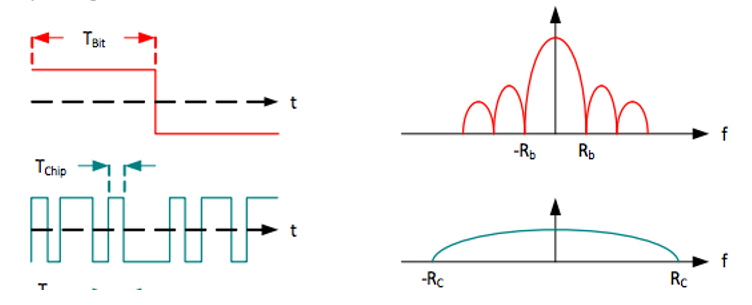
\includegraphics[scale=0.5]{image/hinh2_1}
    \end{center}
    \caption{Nguyên lý điều chế dữ liệu của công nghệ LoRa}
    \label{refhinh2_1}
    \end{figure}
\end{center}
\par
Nhờ sử dụng tín hiệu chirp  mà các tín hiệu LoRa với các tỷ lệ chirp khác nhau có thể hoạt động trong cùng 1 khu vực mà không gây nhiễu cho nhau. Điều này cho phép nhiều thiết bị LoRa có thể trao đổi dữ liệu trên nhiều kênh đồng thời (mỗi kênh cho 1 chirprate).
\subsection{Kiến trúc mạng LoRa}
Một mạng sử dụng công nghệ truyền thông LoRa \cite{4} sẽ được triển khai theo cấu trúc hình sao và gồm hai phần là back-end và front-end (Hình \ref{refhinh2_2}). Phần back-end là máy chủ mạng chứa thông tin nhận được từ các cảm biến. Còn phần front-end chứa module Gateway và các nút (end-device nodes). Gateway có nhiệm vụ làm cầu nối giữa các nút và máy chủ. Thông tin mà Gateway nhận được sẽ được gửi đến máy chủ qua kết nối IP.
\begin{center}
    \begin{figure}[h]
    \begin{center}
     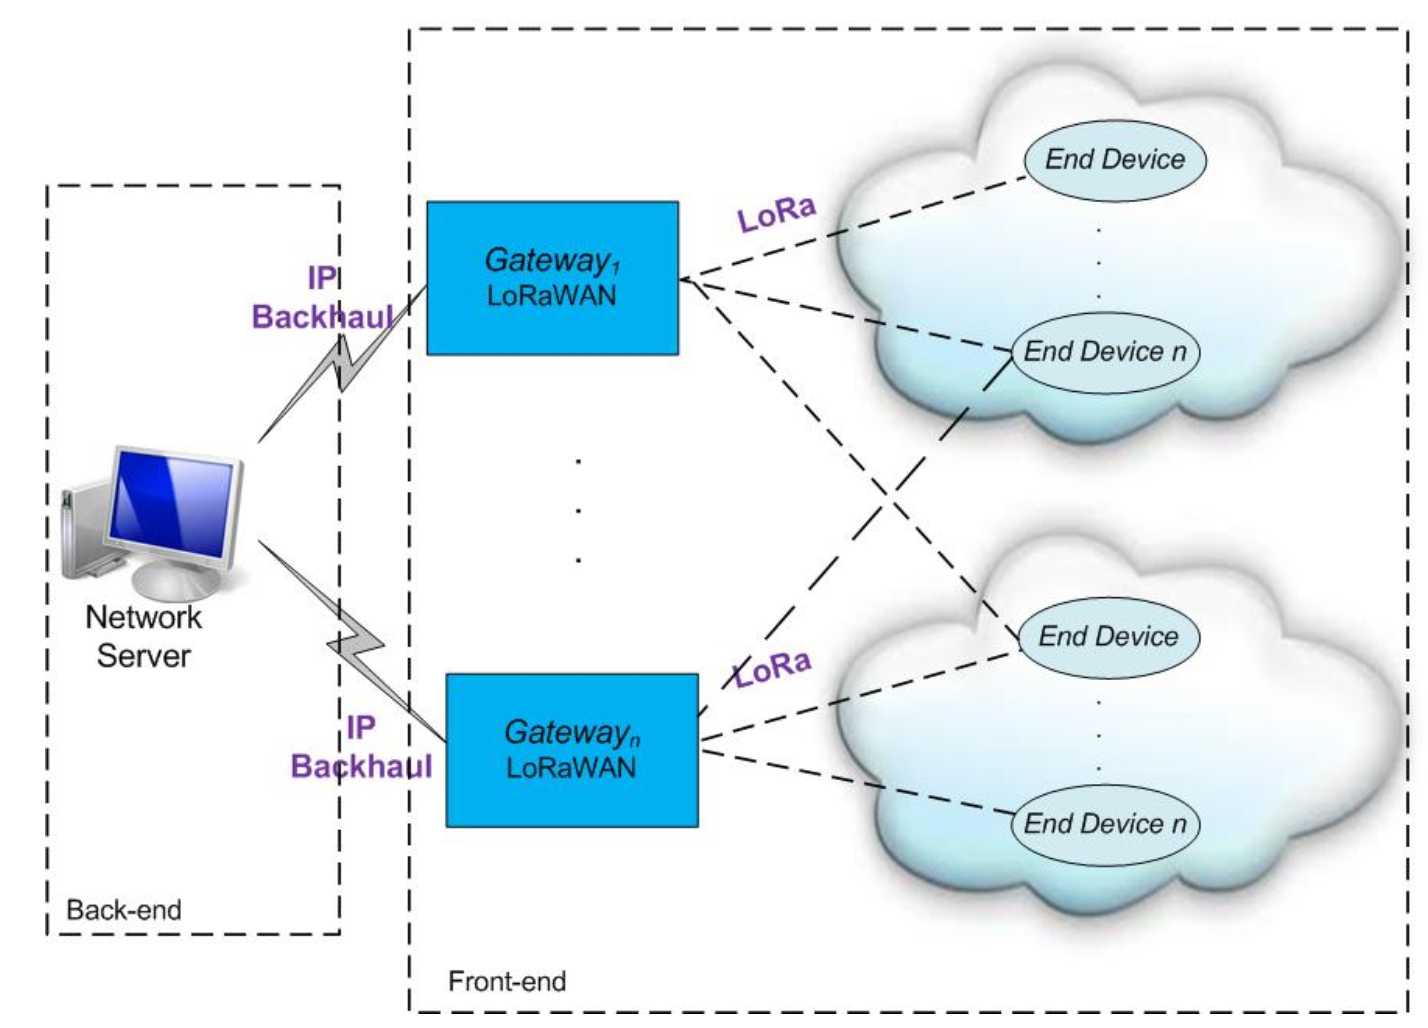
\includegraphics[scale=0.22]{image/hinh2_2}
    \end{center}
    \caption{Kiến trúc mạng LoRa \cite{4}}
    \label{refhinh2_2}
    \end{figure}
\end{center}
\par 
LoRa hoạt động dải tần ISM \cite{4}, tuy nhiên ở mỗi nước (khu vực) thì dải tần này lại khác nhau. Cụ thể là:
\begin{itemize}
\item	Ở Châu Âu, dải tần ISM là: 433MHz hoặc 863-870MHz, gồm có 3 kênh (tương ứng với mỗi dải tần): 433.175 MHz, 433.375 MHz, 433.575 MHz hoặc 868.10 MHz, 868.30 MHz, 868.50 MHz,
\item	Dải tần ISM ở Mỹ là: 902-928MHz,
\item 	Dải tần ISM ở Trung Quốc là: 779-787MHz,
\item 	Ở Úc, dải tần ISM là: 915-928MHz.
\end{itemize}
\par 
Dựa vào cơ chế truyền thông, các nút LoRa (end-device) được chia thành 3 loại \cite{4} gồm:
\begin{itemize}
\item	Class A (Baseline): Khung truyền được chia thành uplink và downlink, bao gồm 1 khe thời gian uplink, tiếp theo là 2 khe thời gian downlink. Thiết bị loại này chỉ có thể nhận dữ liệu từ máy chủ sau khi nó đã gửi dữ liệu,
\item Class B (Beacon): Thiết bị đầu cuối mở thêm một khe nhận trong khoảng thời gian downlink, cùng thêm hai khe thời gian được chỉ định trong loại A. Ngoài khả năng nhận dữ liệu như các thiết bị loại A, các thiết bị loại B cũng có thể sử dụng một loạt khe nhận được kích hoạt bởi các bản tin kiểu Beacon đươc gửi từ gateway,
\item	Class C (Continuous): Các thiết bị loại này có thể nhận dữ liệu bất kể khi nào trừ lúc truyền dữ liệu.
\end{itemize}
    \begin{figure}[h]
    \begin{center}
     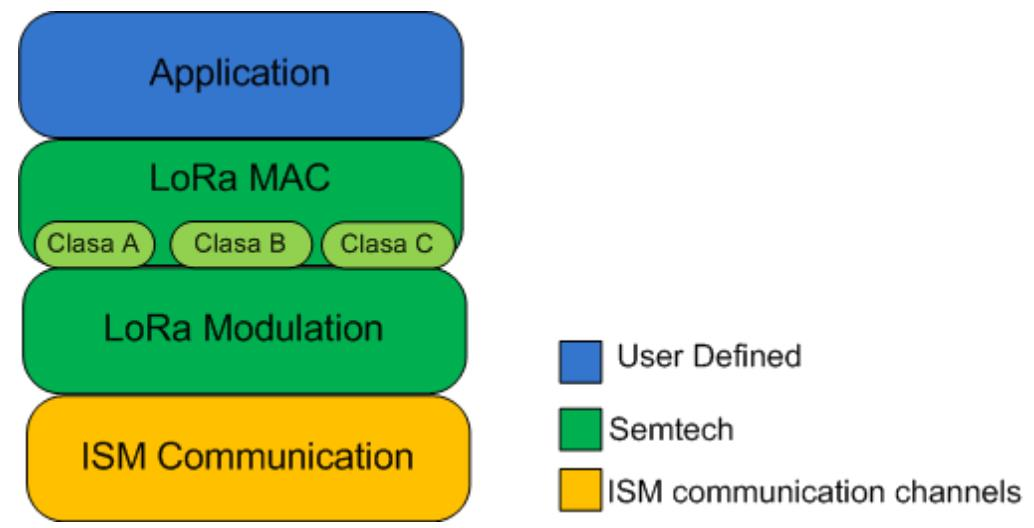
\includegraphics[scale=0.43]{image/hinh2_3}
    \end{center}
    \caption{Kiến trúc các lớp của thiết bị LoRa \cite{4}}
    \label{refhinh2_3}
    \end{figure}
Thiết bị loại A là đơn giản nhất và đảm bảo tiêu thụ năng lượng tối thiểu nhưng lại bị hạn chế khả năng nhận tin nhắn. Nên theo tiêu chuẩn LoRa, các thiết bị phải thực hiện tối thiểu được cơ chế truyền thông loại A. Hình \ref{refhinh2_3} sẽ cho ta thấy rõ hơn cấu trúc các lớp của một thiết bị LoRa.
\subsection{Thông số hoạt động chính của LoRa}
Đối với chipset SX1278 của Semtech, hệ số trải phổ SF (Spreading Factor) có giá trị từ 7 đến 12 \cite{5}. Hệ số SF thể hiện mối quan hệ giữa tốc độ truyền dữ liệu và khoảng cách truyền. Lựa chọn hệ số SF cao có thể làm tăng phạm vi hoạt động nhưng giảm tốc độ truyền dữ liệu và ngược lại. Mỗi ký hiệu được mã hóa bởi một mã có độ dài $2^{SF}$ chip. Do việc mã hóa một ký hiệu bằng nhiều tín hiệu chip, điều này làm ảnh hưởng đến tốc độ truyền dữ liệu. Mỗi quan hệ giữa tốc độ truyền dữ liệu và hệ số SF được thể hiện trong Hình \ref{refhinh2_4}{}a tại các băng thông khác nhau.\\
\begin{figure}[h]
\centering
\subfigure[Tốc độ truyền dữ liệu tương ứng với mỗi hệ số SF.]
  {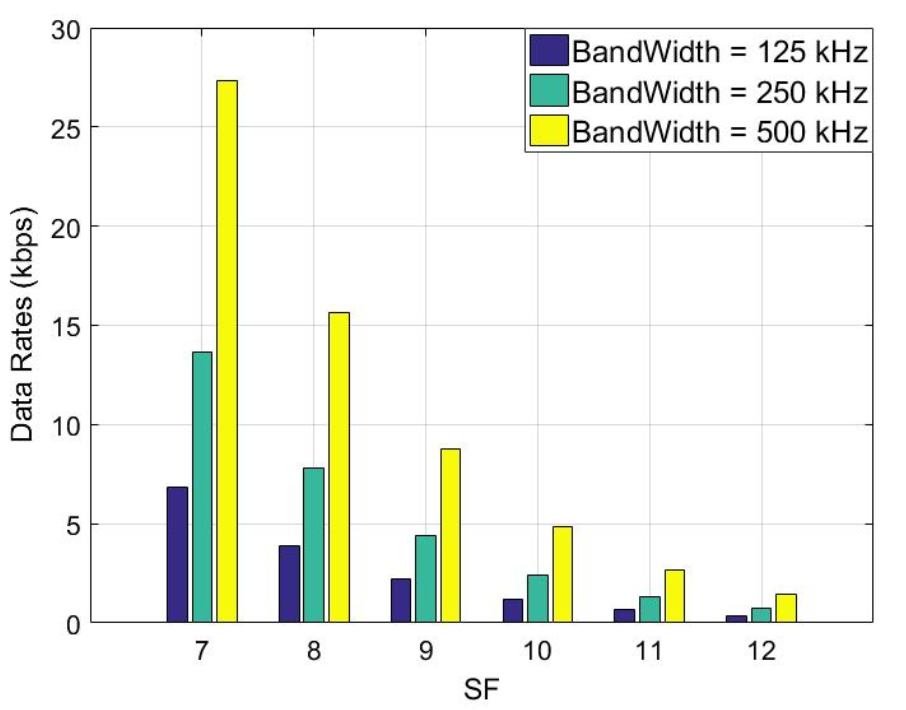
\includegraphics[width=.49\linewidth]{image/hinh2_4}}\hfill
\subfigure[Tốc độ truyền dữ liệu tương ứng với mỗi tốc độ CR.]
  {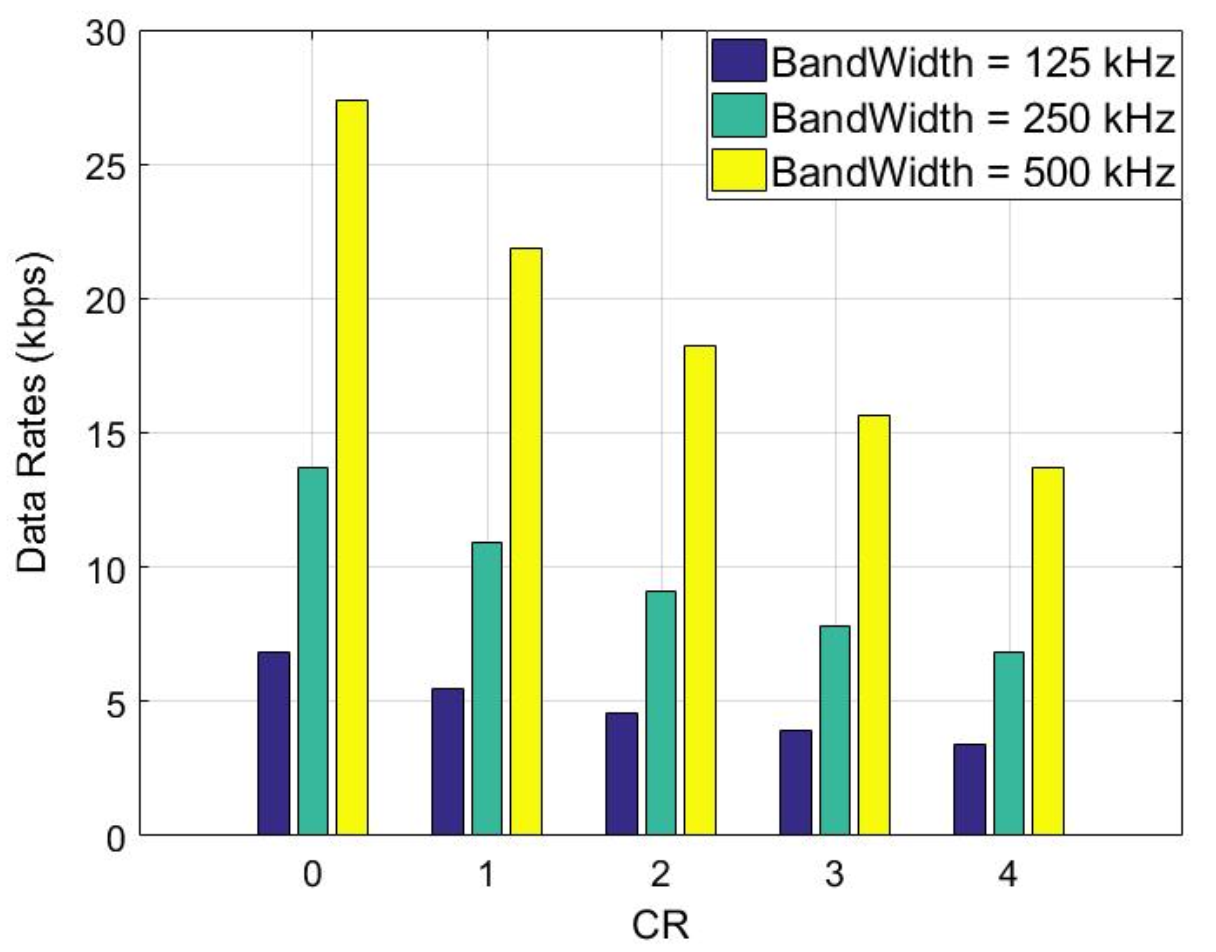
\includegraphics[width=.49\linewidth]{image/hinh2_5}}
\caption{Mối quan hệ giữa tốc độ truyền dữ liệu với các hệ số SF, CR \cite{5}}
\label{refhinh2_4}
\end{figure}
\par 
Theo tài liệu \cite{5}, LoRa thường sử dụng băng thông BW  Bandwidth) có giá trị là 125 KHz nhưng cũng có thể mở rộng lên thành 250 KHz và 500 KHz để truyền tín hiệu. Với băng thông có độ rộng lớn, LoRa hạn chế được nhiễu kênh truyền, hiệu ứng doppler và fading. Máy phát gửi dữ liệu với tốc độ chip bằng với băng thông nên với băng thông là 125 kHz thì tốc độ chip là 125 kcps.
\par 
Tốc độ mã hóa CR (Coding Rate) của chipset SX1278 của SemTech thì CR có 4 giá trị là 4/5, 4/6, 4/7 và 4/8. Nếu tốc độ mã hóa là k/n, thì k là số bit có ích (chứa thông tin được mã hóa) và n là số bit ở đầu ra. Do đó n - k là số bit dự phòng, những bit này cho phép người nhận phát hiện và sửa lỗi trong bản tin nhưng nó cũng làm giảm tốc độ truyền dữ liệu. Tốc độ truyền dữ liệu tương ứng với mỗi CR được thể hiện trong Hình \ref{refhinh2_4}{}b ở mỗi băng thông khác nhau. Ngoài ra, tốc độ truyền dữ liệu cũng phụ thuộc vào độ dài gói tin (Hình \ref{refhinh2_6}). \\
\begin{figure}[h]
\centering
\subfigure[Thời gian truyền gói tin với BW = 125 kHz and CR = 0.]
  {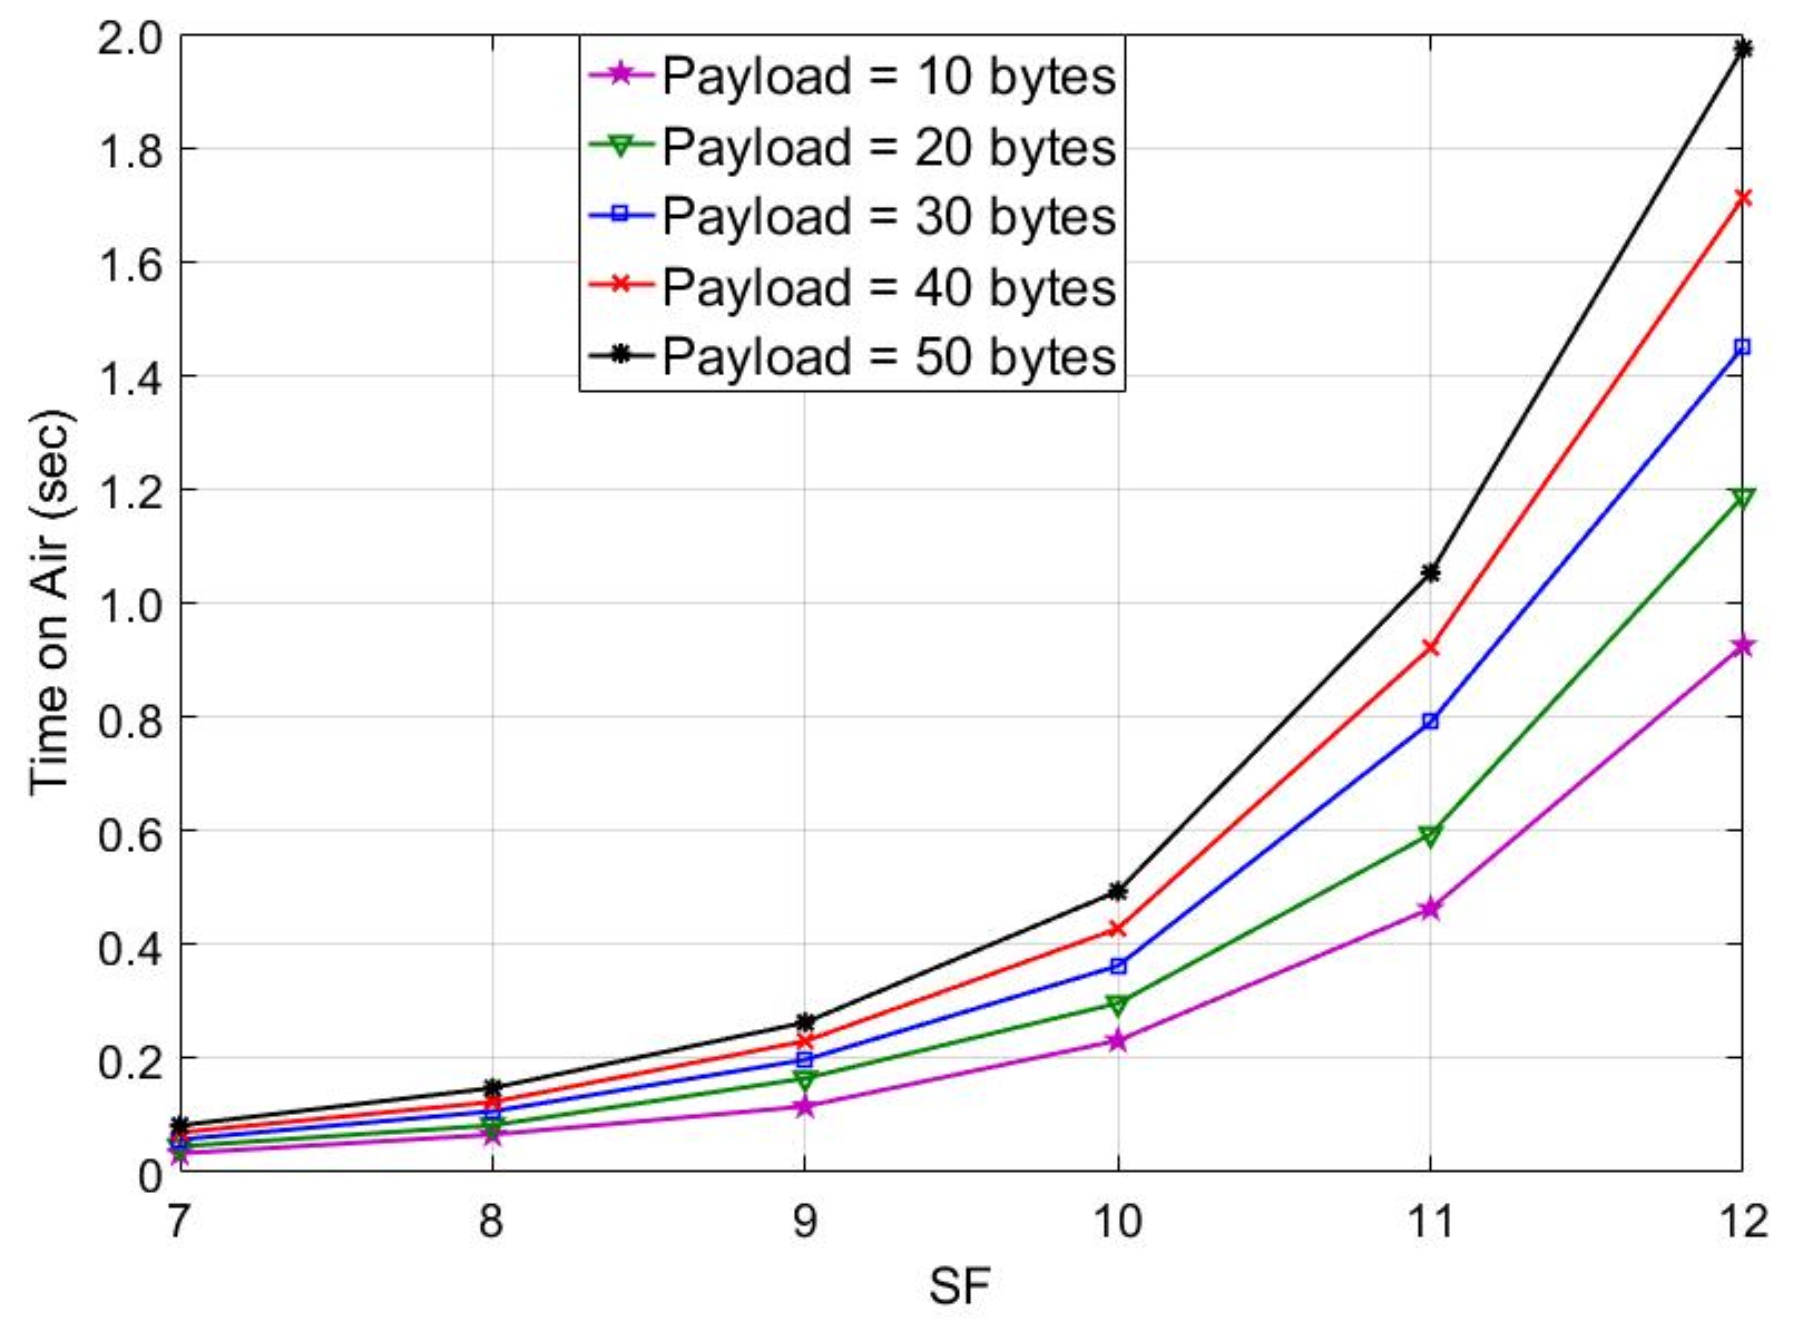
\includegraphics[width=.49\linewidth]{image/hinh2_7a}}\hfill
\subfigure[Thời gian truyền gói tin với BW = 125 kHz and CR = 02.]
  {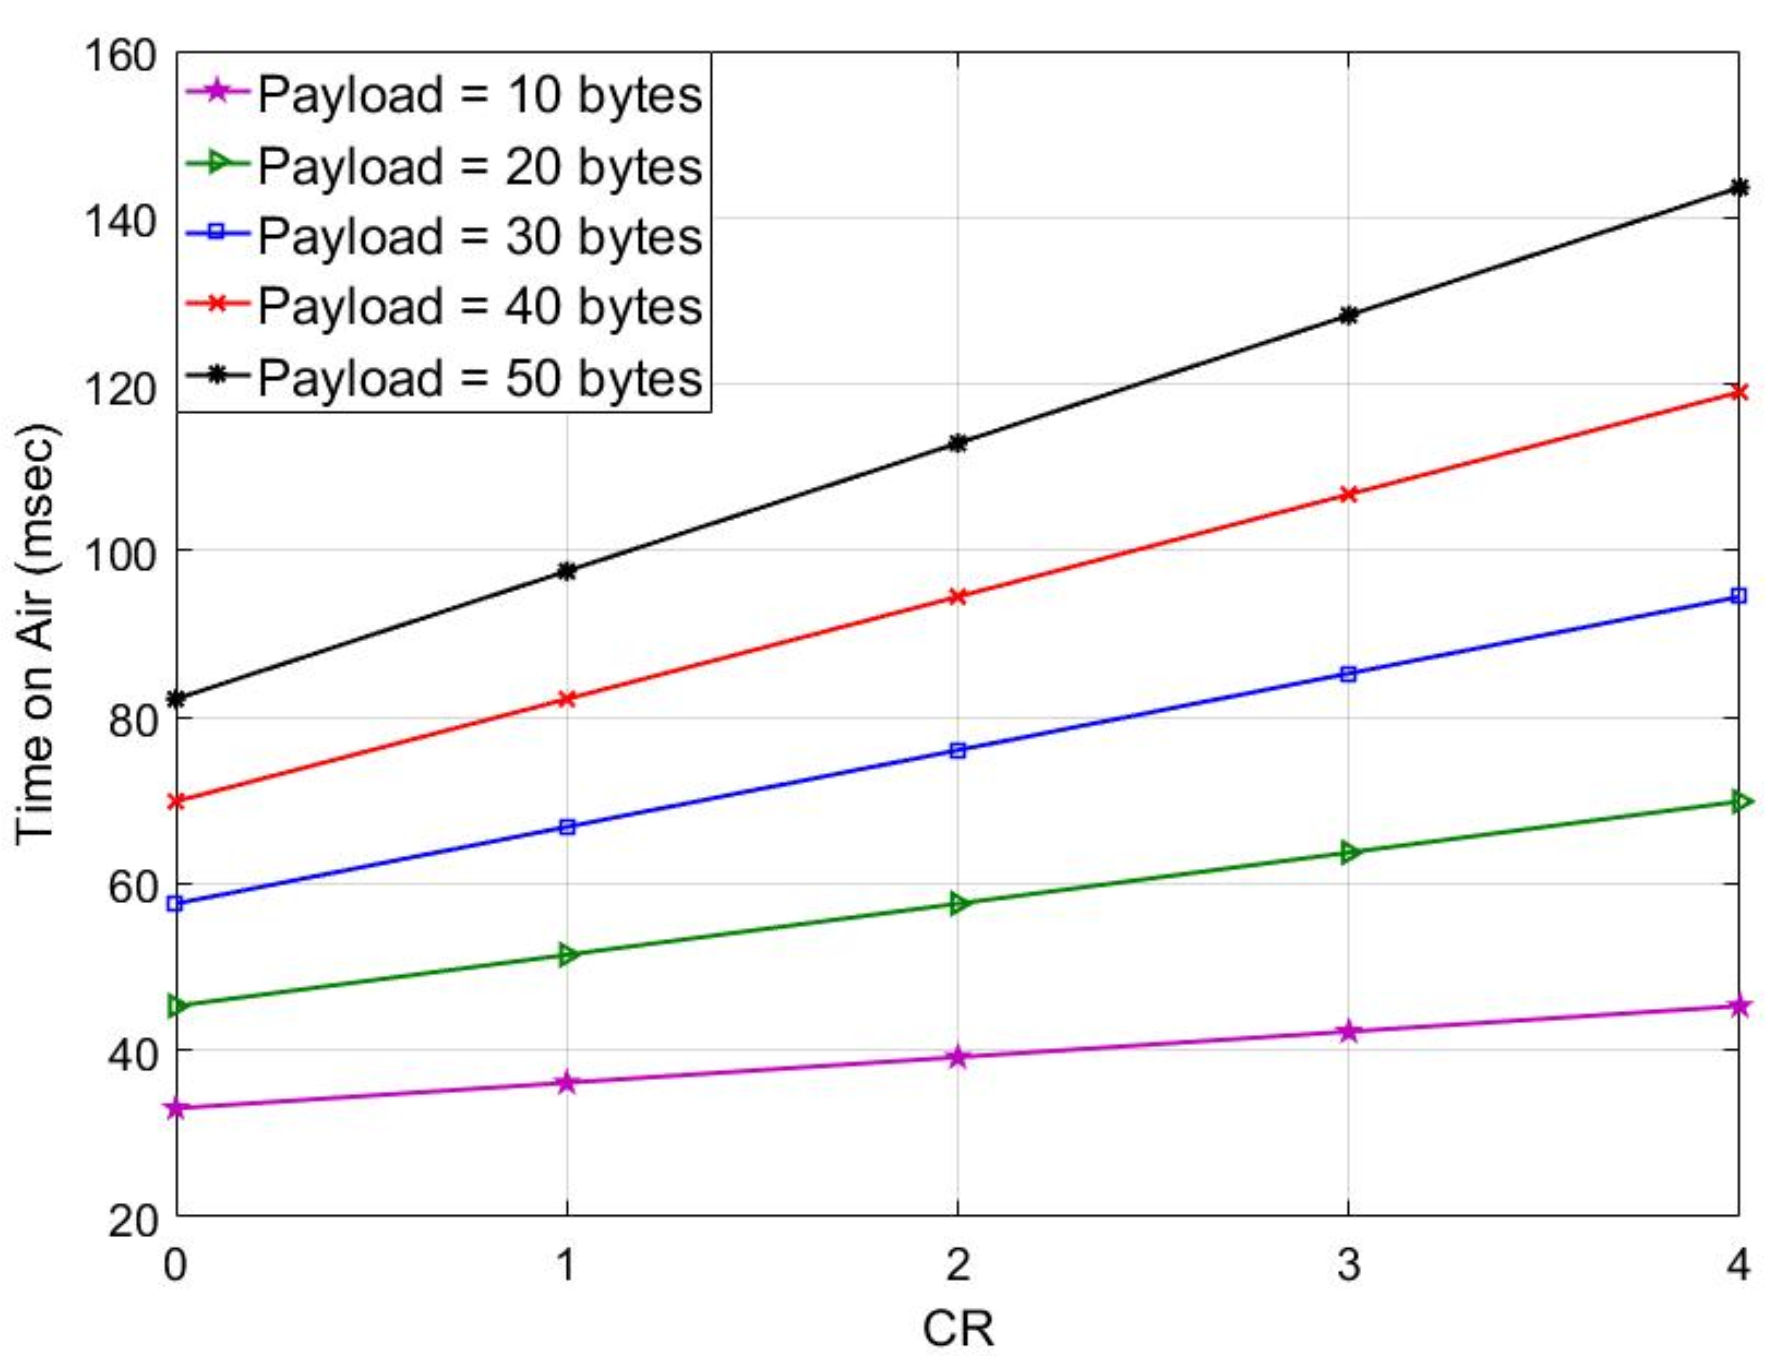
\includegraphics[width=.49\linewidth]{image/hinh2_7b}}
\caption{Thời gian truyền gói tin trong không khí của LoRa. \cite{5}}
\label{refhinh2_6}
\end{figure} 
\begin{center}
    \begin{figure}[h]
    \begin{center}
     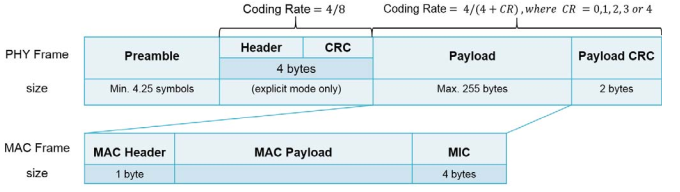
\includegraphics[scale=0.6]{image/hinh2_6}
    \end{center}
    \caption{Cấu trúc một gói dữ liệu được truyền đi \cite{5}.}
    \label{refhinh2_5}
    \end{figure}
\end{center}
\par
Kích thước lớn nhất của một gói tin LoRa là 256 byte, cấu trúc một gói tin (Hình \ref{refhinh2_5}{}) gồm các thành phần sau:
\begin{itemize}
\item  Preamble: là trường chuỗi bit để dò tìm tín hiệu của LoRa trong không gian,\newline
\item  Header: chứa thông tin về kích thước của Playload và xem có Payload CRC hay không. Giá trị của Header cũng được check CRC kèm theo,
\item  Payload: chứa dữ liệu ứng dụng truyền qua LoRa, có kích thước từ 2 đến 255 byte. Trường này còn chứa các trường sau:
	\begin{itemize}
	\item	MAC header: phụ thuộc vào kiểu của frame (là dữ liệu hoặc ACK), phiên bản của giao thức và hướng của nó (uplink hoặc downlink).
	\item	MAC payload: chứa dữ liệu.
	\item 	MIC: được sử dụng như là chữ ký số của dữ liệu.
	\end{itemize}
\item	CRC: là trường tùy chọn và chứa các byte kiểm tra vòng CRC (Cyclic Redundancy Check).
\end{itemize}
\section{Đa truy nhập trong mạng không dây}
Đa truy nhập (Multiple Access) là một kỹ thuật cho phép nhiều thiết bị sử dụng chung một kênh truyền. Kỹ thuật này nằm ở lớp MAC (Medium Access Control), đây là một lớp đặc biệt quan trọng trong những mạng LAN (Local Area Network), trong đó có mạng không dây bởi vì các thiết bị trong mạng này sử dụng chung môi trường truyền.
\par
Giả sử có nhiều thiết bị đang sử dụng kênh truyền, trong cùng một khoảng thời gian với cùng tần số, khi đó sẽ xảy ra hiện tượng va chạm. Do đó, cần phải có một biện pháp kiểm soát các thiết bị tham gia kênh truyền. Ví dụ như một mạng có băng thông là B, có N thiết bị đang tham gia kênh truyền, mạng sử dụng phương pháp ghép kênh phân chia theo tần số FDM (Frequency Division Multiplexing), khi đó băng thông được chia thành N dải tần, mỗi thiết bị sẽ sử dụng một dải tần. Tuy nhiên, với số lượng thiết bị lớn, thì những dải tần này bị chia quá nhỏ, do đó dễ gây nên can nhiễu. Do đó, cần có thêm những phương pháp kiểm soát kênh truyền. Đây là 4 phương pháp điều khiển truy nhập kênh truyền:
\begin{itemize}
\item Đa truy nhập phân chia theo tần số FDMA (Frequency Division Multiple Access): dải tần số sẽ được chia thành các dải tần số nhỏ không chồng lên nhau, và mỗi dải đó được sử dụng bởi một thiết bị khác nhau, 
\item Đa truy nhập phân chia theo thời gian TDMA (Time Division Multiple Access): mỗi thiết bị trong mạng sử dụng chung một dải tần nhưng chỉ được phép truyền trong một khoảng thời gian cụ thể,
\item Đa truy nhập phân chia theo mã CDMA (Code Division Multiple Access): các thiết bị trong mạng sẽ sử dụng chung một dải tần và có thể gửi bản tin cùng một thời gian nhưng những tín hiệu đó sẽ được mã hóa bằng các mã ngẫu nhiên khác nhau,
\item Đa truy nhập phân chia theo không gian SDMA (Space Division Multiple Access): các thiết bị trong mạng sẽ sử dụng chung một dải tần, truyền/nhận bản tin cùng một lúc và không sử dụng mã ngẫu nhiên để mã hóa. Tại trạm cơ sở, yêu cầu phải có một dãy ăng-ten lớn để khử nhiễu. 
\end{itemize}
Từ những phương pháp điều khiển kênh truyền trên, các giao thức đa truy nhập đã được phát triển.
\subsection{ALOHA}
Theo tài liệu \cite{6}, giao thức đa truy nhập đầu tiên bắt đầu một cách sơ khai ở Hawaii vào đầu những năm 1970, do Norman Abramson đề xuất. Gọi là "sơ khai" bởi vì nó không được sử dụng cho mạng di động. Mục đích của Norman Abramson và các cộng sự khi tạo ra mạng này để kết nối những thiết bị ở những hòn đảo xa tới máy chủ ở Honolulu. Sau đó, công trình của ông, hệ thống pure ALOHA (ALOHA nguyên thủy), đã thu hút sự chú ý của rất nhiều nhà nghiên cứu và nó đã được phát triển thêm thành giao thức slotted ALOHA.
\subsubsection{Pure ALOHA}
Ý tưởng của hệ thống ALOHA là rất đơn giản: người sử dụng sẽ truyền bản tin bất khi nào họ có dữ liệu. Do đó, va chạm trong ALOHA là điều dễ hiểu. Trong hệ thống ALOHA, sau khi trạm đã gửi bản tin của nó đến máy chủ, máy chủ sẽ phát quảng bá bản tin đó đến tất cả các trạm. Trạm gửi bản tin có thể biết được máy chủ đã nhận được bản tin của nó hoặc bản tin được gửi đã đúng chưa qua việc nhận lại bản tin từ máy chủ. Nếu việc gửi không thành công, bên gửi sẽ chờ một khoảng thời gian ngẫu nhiên nào đó rồi gửi lại. Thời gian chờ này phải ngẫu nhiên để tránh việc va chạm với bản tin quay trở lại từ máy chủ. Khi hệ thống có nhiều thiết bị cùng chia sẻ một kênh, điều đó dẫn đến việc xung đột kênh truyền. Hình \ref{aloha_conflict} mô tả quá trình gửi bản tin một cách tùy ý trong hệ thống ALOHA.\\
\begin{figure}[htp]
\begin{center}
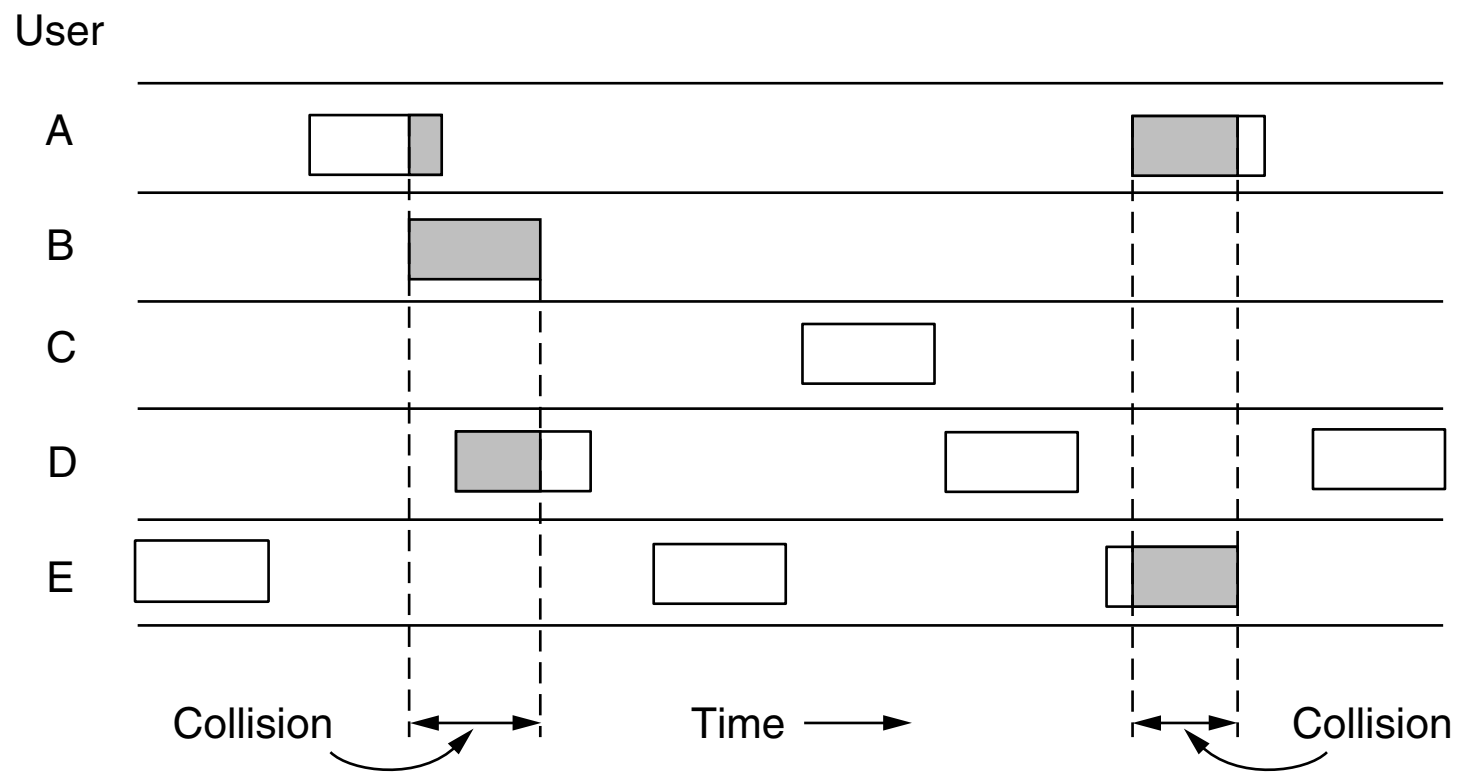
\includegraphics[scale=0.26]{image/aloha_conflict}
\end{center}
\caption{Các gói tin được truyền trong ALOHA \cite{6}}
\label{aloha_conflict}
\end{figure}
\begin{figure}[h]
\begin{center}
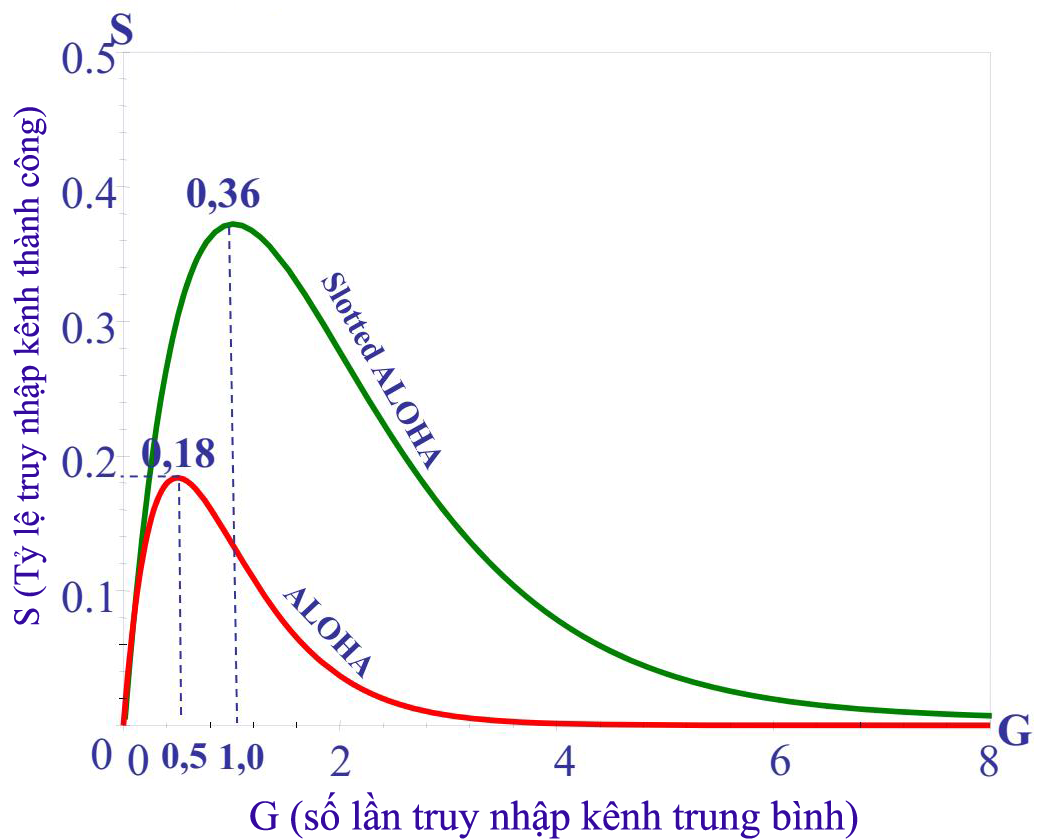
\includegraphics[scale=0.3]{image/efficiency_aloha}
\end{center}
\caption{Hiệu năng của hai giao thức ALOHA và Slotted ALOHA}
\label{efficiency_aloha}
\end{figure}
\par 
Do không có cách nào để kiểm soát xung đột trong ALOHA, nên hiệu năng của giao thức này khá thấp như thể hiện trong Hình \ref{efficiency_aloha}{}.
\subsubsection{Slotted Aloha}
Theo tài liệu \cite{6}, ngay sau ALOHA, vào năm 1972, Roberts đã công bố một phương pháp giúp tăng gấp đôi hiệu năng của hệ thống ALOHA. Đề xuất của ông là chia thời gian thành những khe thời gian rời rạc gọi là slot, bắt đầu của mỗi khe thời gian là lúc cho mỗi trạm tham gia kênh truyền. Phương pháp này yêu cầu các trạm phải thống nhất với nhau về khe thời gian. Một cách để có sự đồng bộ này là một trạm đặc biệt sẽ phát ra tín hiệu để thông báo bắt đầu khe thời gian. Hiệu năng của Slotted Aloha được mô tả trong Hình \ref{efficiency_aloha}{}.
\par 
Trong nắng năm 1970, sau khi được tạo ra, Slotted ALOHA được sử dụng trong các thí nghiêm và rồi nhanh chóng bị lãng quên cũng như ALOHA.
\subsection{Giao thức đa truy nhập dựa vào việc kiểm tra kênh truyền} 
Khi một trạm truyền bản tin, nó sẽ không biết các trạm khác đang làm gì, do vậy ở vùng giao của vùng phát sóng hai trạm sẽ xảy ra nhiều xung đột. Do đó, cần có một giao thức mà trạm có thể cảm nhận được kênh truyền. Có nhiều giao thức nghe kênh truyền đã được đưa ra, sau đây em xin trình bày một số phiên bản của giao thức đa truy nhập dựa vào việc cảm nhận kênh truyền CSMA (Carrier Sense Multiple Access).
\subsubsection{1-persistent CSMA}
1-persistent CSMA \cite{6} là giao thức đơn giản nhất trong các giao thức CSMA. Khi trạm có dữ liệu, đầu tiền nó sẽ cảm nhận kênh truyền xem các trạm khác có đang gửi tin không. Nếu kênh truyền rảnh, trạm sẽ gửi dữ liệu. Ngược lại, nếu kênh truyền bận, trạm sẽ chờ đến khi kênh truyền rảnh. Sau đó trạm sẽ truyền bản tin. Nếu va trạm xảy ra, trạm sẽ chờ một khoảng thời gian ngẫu nhiêu và bắt đầu gửi lại. Quá trình gửi tin của trạm sẽ được mô tả trong lưu đồ thuật toán Hình \ref{2CSMA}{}a. Tuy nhiên, trong trường hợp hai trạm cùng chờ chạm thức 3 thực hiện xong quá trình gửi tin, khi đó hai trạm sẽ cùng gửi tin, xung đột sẽ xảy ra. Giao thức 1-persistent CSMA có hiệu năng tốt hơn so với ALOHA do có quá trình kiểm tra kênh truyền.\\
\begin{figure}[h]
\centering
\subfigure[1-persistent CSMA.]
  {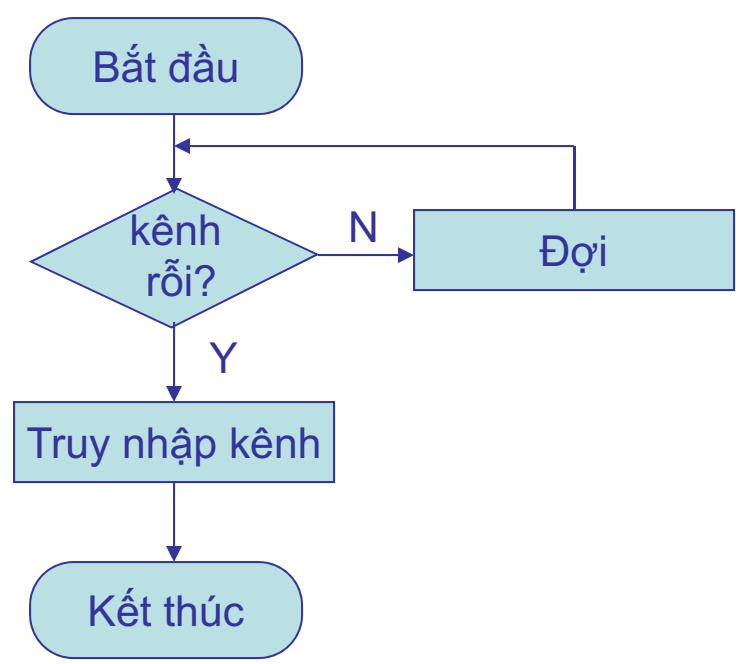
\includegraphics[width=.42\linewidth]{image/flowchart_1per}}
\hfill
\subfigure[non-persistent CSMA.]
  {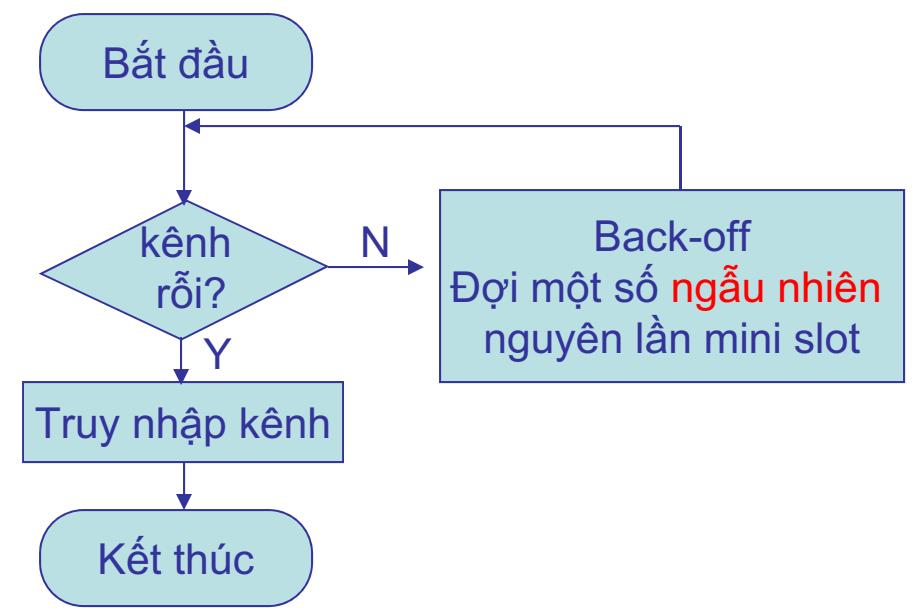
\includegraphics[width=.55\linewidth]{image/flowchart_nonper}}
\caption{Lưu đồ thuật toán của hai giao thức 1-persistent CSMA và non-persistent CSMA}
\label{2CSMA}
\end{figure} 
\subsubsection{Non-persistent CSMA}
Giao thức kiểm tra kênh truyền thức hai là nonpersistent CSMA. Theo tài liệu \cite{6}, cũng giống như 1-persistent CSMA, khi cảm nhận được kênh truyền rỗi, trạm sẽ gửi luôn bản tin. Tuy nhiên, khi kênh truyền bận, trạm sẽ không tiếp tục cảm nhận kênh truyền nữa mục đích để không cần ngay lập tức xác định thời điểm kết thúc của quá trình truyền tin trước. Thay vào đó, nó sẽ chờ một khoảng thời gian ngẫu nhiên rồi tiếp tục thuật toán. Hệ quả của quá trình này là sử dụng kênh truyền tốt hơn nhưng thời gian trễ dài hơn so với 1-persistent CSMA. Lưu đồ thuật toán Hình \ref{2CSMA}{}b mô tả giao thức nonpersistent CSMA.
\subsubsection{p-persistent CSMA}
Giao thức p-persistent CSMA \cite{6} khắc phục những nhược điểm của 1-persistent CSMA. Khi trạm sẵn sàng gửi dữ liệu, nó sẽ kiểm tra kênh truyền. Nếu kênh truyền rảnh, nó sẽ gửi dữ liệu với một xác xuất p hoặc đợi một mini slot (mini slot là khoảng thời gian nhỏ hơn rất nhiều so với thời gian truyền tối đa của tín hiệu) với xác xuất q = 1 - p sau đó kiểm tra lại kênh truyền. Khi kênh bận thì đợi kênh rỗi. Hình \ref{flowchart_pper} mô tả thuật toán của giao thức p-persistent CSMA. Giá trị xác suất p ảnh hưởng nhiều đến hiệu suất của kênh truyền.
\begin{figure}[h]
\begin{center}
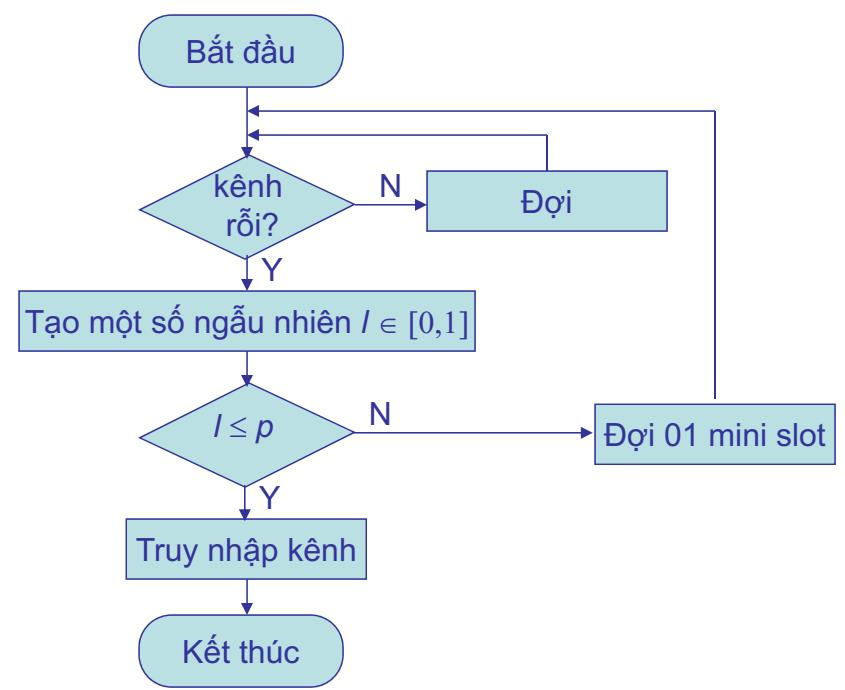
\includegraphics[scale=0.45]{image/flowchart_pper}
\end{center}
\caption{Lưu đồ thuật toán giao thức p-persistent CSMA.}
\label{flowchart_pper}
%\end{figure}//
%\begin{figure}
\begin{center}
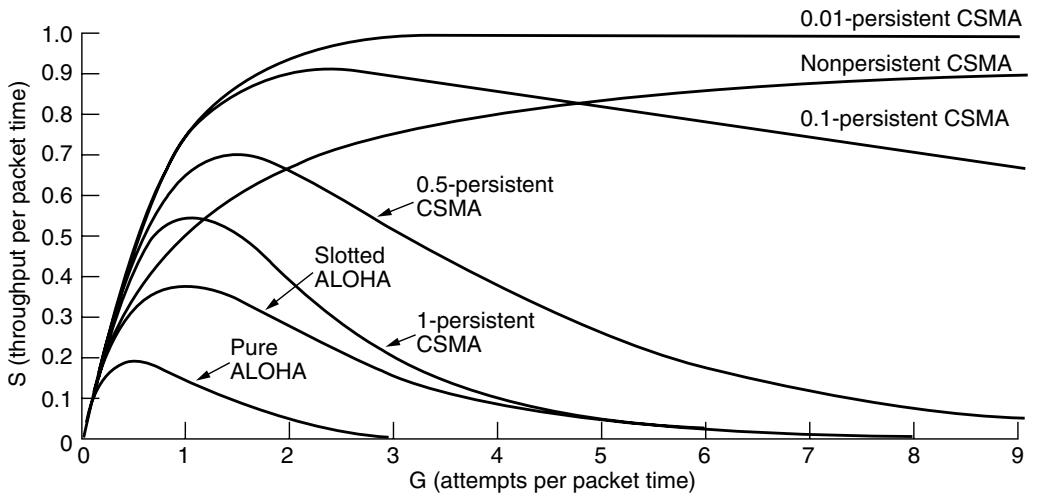
\includegraphics[scale=0.48]{image/compare}
\end{center}
\caption{So sánh hiệu năng sử dụng kênh truyền của các phương pháp truy nhập kênh truyền ngẫy nhiên \cite{6}{}.}
\label{compare}
\end{figure}
\par
Hình \ref{compare} so sánh hiệu suất của 3 giao thức 1-persistent CSMA, nonpersistent CSMA, p-persistent CSMA cũng như ALOHA và slotted ALOHA.
\subsubsection{CSMA/CA}
\begin{figure}[h]
\begin{center}
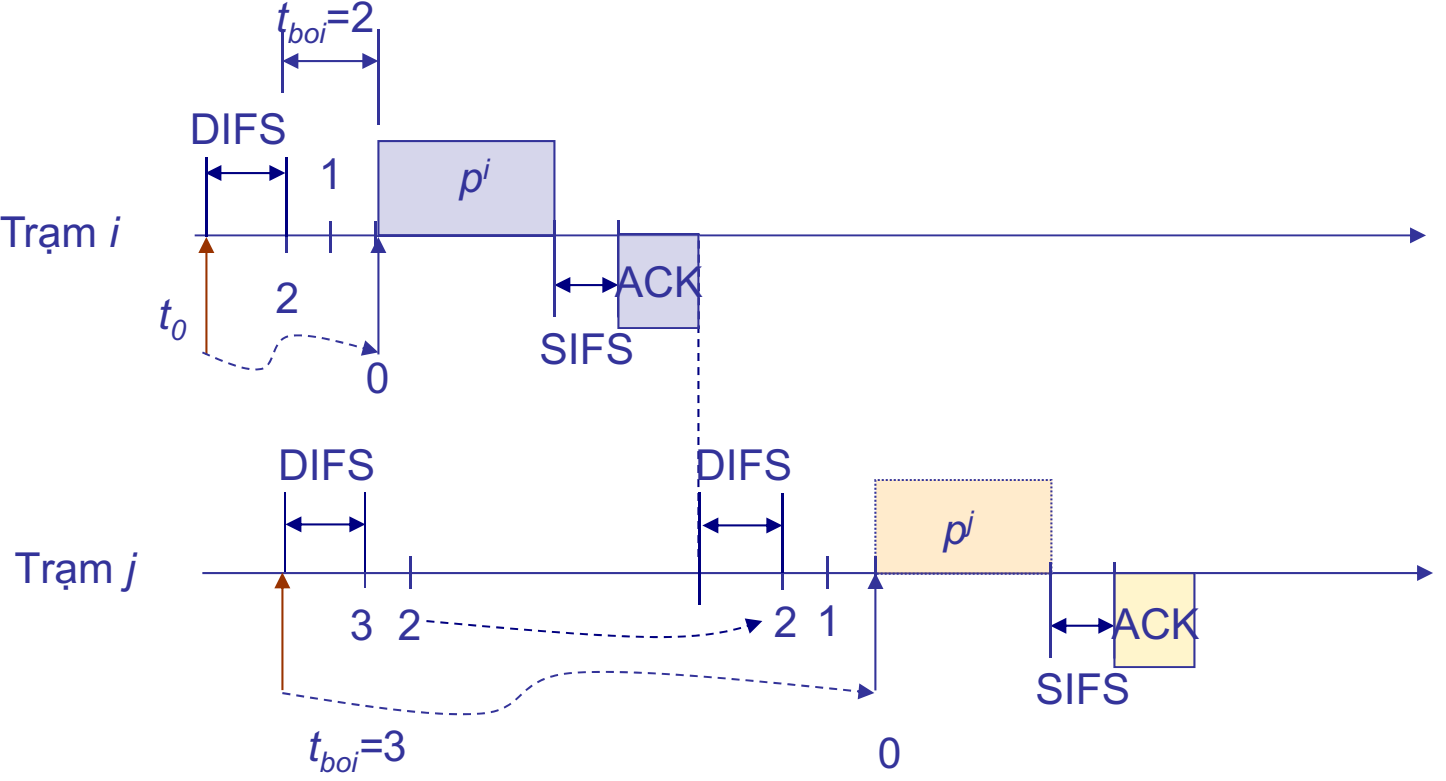
\includegraphics[scale=0.26]{image/CSMACA}
\end{center}
\caption{Quá trình truyền tin của 2 trạm sử dụng giao thức CSMA/CA}
\label{CSMACA}
\end{figure}
\noindent Do cơ chế kiểm tra trạng thái kênh truyền và cơ chế phát hiện va đập hoạt động không hiệu quả trong môi trường vô tuyền, nên cần có một giao thức CSMA được phát triển trong mạng vô tuyến đó là CSMA/CA (CSMA with Collision Avoidance). Cơ chế hoạt động của CSMA/CA (Hình \ref{CSMACA}{}):
\begin{itemize}
\item Trước khi truy nhập kênh truyền, kiểm tra trạng thái kênh truyền. Nếu xảy ra va đập, các trạm sẽ dừng truyền tin và gửi bản tin JAM SIGNAL để báo hiệu cho các trạm khác và back-off theo hàm mũ. Điều này có nghĩa, số lần truy nhập kênh truyền không thành công càng lớn thì thời gian back-off càng tăng,
\item Nếu kênh truyền bận: đợi đến khi kênh truyền rỗi,
\item Tiếp tục đợi thêm khoảng thời gian DIFS (DCF Inter-Frame Space) cho trước (DIFS = RTT),
\item Back-off một số mini slot $t_{BO}$ ngẫu nhiên,
\item Sau mỗi mini slot: $t_{BO} = t_{BO} - 1${},
\item  Nếu trong thời gian back-off kênh truyền lại bận thì trạm dừng đếm lùi và bảo toàn giá trị $t_{BO}$ tại thời điểm dừng,
\item Sau khi kênh truyền chuyển sang trạng thái rỗi một khoảng thời gian DIFS, trạm tiếp tục đếm lùi,
\item Nếu $t_{BO}$ = 0 thì truy nhập kênh và gửi gói.
\end{itemize}
\subsection{Giao thức đa truy nhập tránh va chạm MACA}
Ý tưởng cơ bản của giao thức MACA \cite{6} (Multiple Access with Collision Avoidance) (Karn, 1990) là sử dụng cơ chế tránh va đập. Quá trình truyền tin của trạm sử dụng giao thức MACA được mô tả trong Hình \ref{MACA}{}. Cơ chế tránh va đập gồm có các thành phần:
\begin{itemize}
\item Trước khi gửi: bên gửi sẽ quảng bá bản tin RTS (Ready-To-Send) cho các nút xung quanh biết là nó sắp sửa gửi bản tin,
\item Khi nhận được RTS: bên thu quảng bá bản tin CTS (Clear-To-Send) để cho bên nhận và các nút xung quanh nó biết nó sẵn sàng nhận bản tin,
\item Trong RTS và CTS mang theo bản tin NAV (Network Allocation Vector) chứa thời gian chiếm kênh truyền của bên phát,
\item Các trạm khác dừng việc truy nhập kênh truyền trong khoảng thời gian NAV.
\end{itemize}
\begin{figure}[h]
\begin{center}
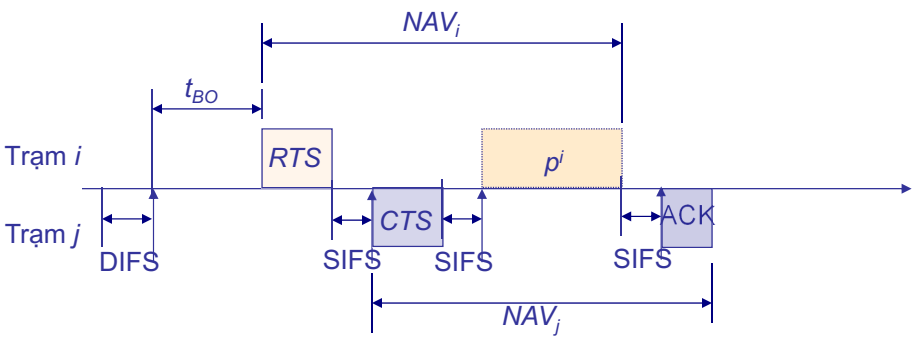
\includegraphics[scale=0.4]{image/MACA}
\end{center}
\caption{Quá trình truyền tin của hai trạm sử dụng giao thức MACA}
\label{MACA}
\end{figure}
Ở trên là một số giao thức đa truy nhập có thể áp dụng cho mạng không dây, mỗi giao thức có những ưu điểm và cũng có nhược điểm riêng. Đối với đề tài của mình, em xin lựa chọn việc xây dựng giao thức đa truy nhập của mình dựa trên giao thức ALOHA. Bởi vì, giao thức ALOHA đơn giản, dễ dàng triển khai. Ngoài ra, do dữ liệu cần truyền là nhỏ (dữ liệu lớn nhất trong một lần truyền là 255 byte), cùng với số lượng nút trong mạng ít nên rất phù hợp với việc ứng dụng giao thức ALOHA.
\section{Module LoRa Ai Thinker SX1278 Ra-02}
Ai Thinker là một hãng chuyên về lĩnh vực thiết kế và sản xuất module truyền thông không dây (WiFi, LoRa, GPRS,…) của Trung Quốc.
\par 
Module truyền thông LoRa SX1278 Ra-02 là một trong số những module sử dụng công nghệ LoRa có giá thành rẻ, sử dụng IC truyền thông LoRa SX1278 của Semtech. Hình ảnh module SX1278 cùng với sơ đồ chân và sơ đồ khối được thể hiện trong Hình \ref{SX1278}.
\begin{figure}[t]
	\centering
	\subfigure[Hình ảnh thực tế Module LoRa Ai Thinker SX1278 Ra-02 \cite{*}]
	{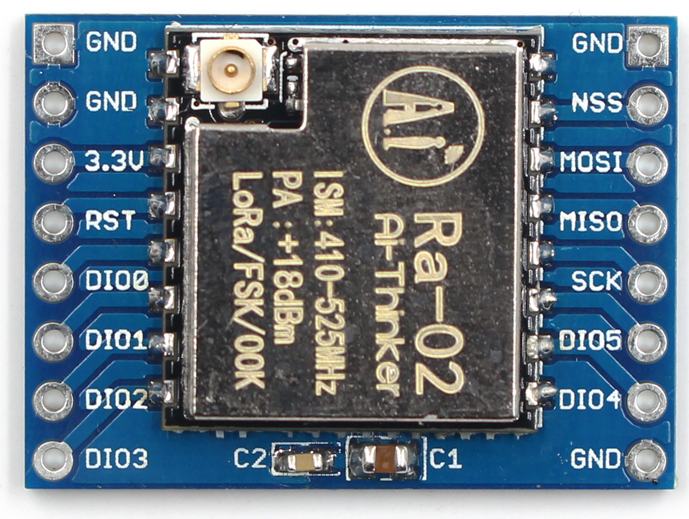
\includegraphics[width=0.45\linewidth]{image/hinh2_7}}
	\subfigure[Sơ đồ chân IC SX1278 \cite{8}]
	{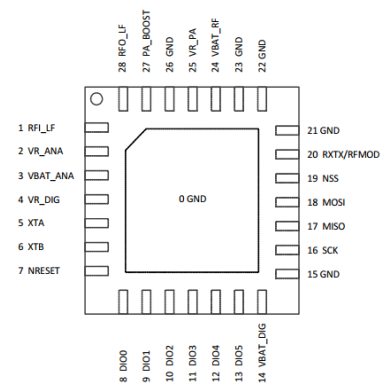
\includegraphics[width=0.46\linewidth]{image/hinh2_9}}\\
	\subfigure[Sơ đồ khối IC SX1278 \cite{8}]
	{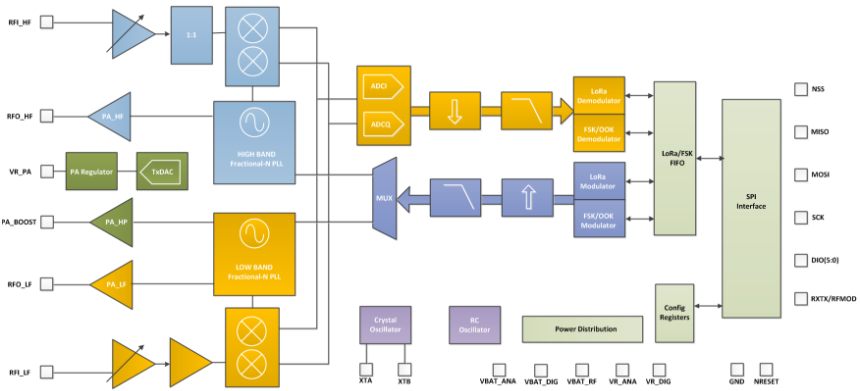
\includegraphics[scale=0.5]{image/hinh2_8}}%
\caption{Module LoRa Ai Thinker SX1278 Ra-02}
\label{SX1278}
\end{figure}
\par 
Thông số của module LoRa Ai Thinker SX1278 Ra-02 \cite{7} gồm có:
\begin{itemize}
\item Kích thước: 17 x 16 mm,
\item Hỗ trợ chuẩn giao tiếp SPI,
\item Hoạt động trên dải tần: 410 – 525 MHz,
\item Hỗ trợ công nghệ điều chế FSK, GFSK, GMSK và LoRa,
\item Điện áp hoạt động: 2.5 – 3.7,
\item Dòng điện tiêu thụ (Bảng \ref{bang2_1}),
\item Công suất phát: 18 $\pm$ 1 dBm,
\item Nhiệt độ hoạt động: -30 - 85 $^{\circ}$C .
\end{itemize}
\begin{table}[h]
    \centering
    \caption{Dòng điện tiêu thụ của module LoRa Ai Thinker SX1278~Ra-02 \cite{7}}
    \begin{tabular}{|c|c|c|c|}
     	\hline
     	Tần số & RX & TX & Standby \\
     	\hline
     	433 MHz & 93 mA & 12,15 mA & 1,6 mA \\
     	\hline
     	470 MHz & 97 mA & 12,15 mA & 1,5 mA \\
     	\hline
    \end{tabular}
    \label{bang2_1}
\end{table}
Theo datasheet của IC SX1278 do Semtech công bố \cite{8}, IC SX1278 là một trong những chip thu phát sóng điện từ sử dụng công nghệ LoRa, cung cấp một vùng phủ sóng rộng, tiêu thụ ít năng lượng và khả năng chống nhiễu tốt.
\section{Vi điều khiển STM32F103}
Vi điều khiển STM32F103 là loại vi điều khiển 32 bit với lõi ARM Cortex-M3 trên kiến trúc RICS của hãng STMicroelectronics (ST). Vi điều khiển lõi được sử dụng rộng rãi trong các thiết bị điện tử - tự động bởi khả năng xử lý vượt trội, kích thước nhỏ, dễ dàng cho việc lập trình. Vi điều khiển lõi ARM Cortex-M3 dựa trên kiến trúc ARMv7-M được thiết kế để tối ưu hóa hiệu suất cho các ứng dụng vi xử lý, có nhiều ngoại vi, khả năng đa kết nối đa năng, tương thích với nhiều công cụ (tools) nạp của nhiều hãng khác nhau, cho phép lập trình và phát triển các ứng dụng một cách nhanh chóng. Vi điều khiển Cortex-M3 tiêu thụ ít điện năng và chi phí thấp, đồng thời cung cấp khả năng tính toán cao. Dưới đây là một số thông số hoạt động của vi điều khiển STM32F103 \cite{9}{}:
\begin{itemize}
\item Tần số cao nhất: 72MHz,
\item Dung lượng bộ nhớ flash: 256 KB,
\item Dung lượng RAM: 48 KB,
\item Dải điện áp 2,0 V – 3,6 V.
\end{itemize}
\begin{center}
    \begin{figure}[h]
    \begin{center}
     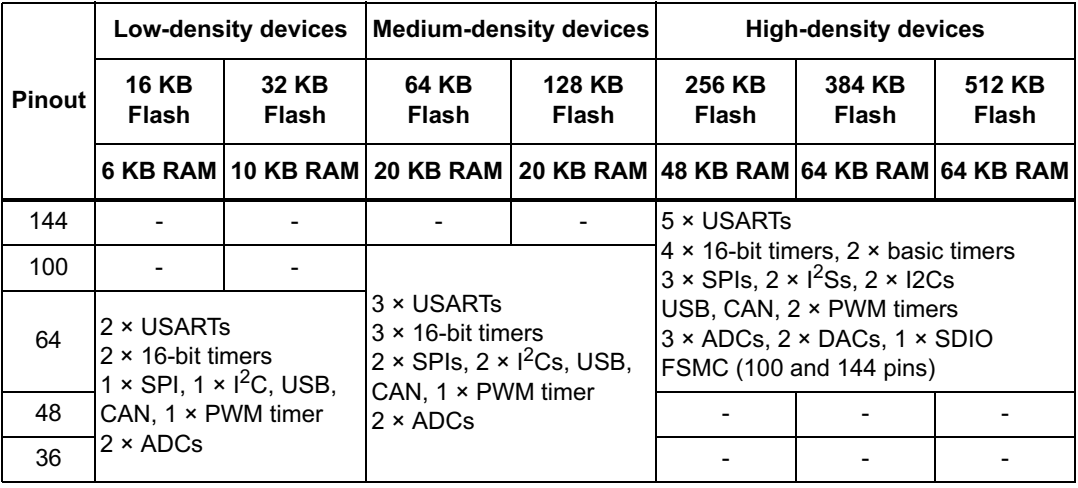
\includegraphics[scale=0.3]{image/bang2_2}
    \end{center}
    \caption{Thông số họ vi điều khiển STM32F103xxx \cite{9}}
    \label{refhinh2_9}
    \end{figure}
\end{center}
\par 
Bên cạnh đó, vi điều khiển STM32F103 còn hỗ trợ các tính năng sau \cite{9}:
\begin{itemize}
\item Bộ chuyển đổ ADC 12-bit,
\item Tích hợp Timer 16-bit với hai bộ điều khiển PWM,
\item Đầy đủ các kết nối thông dụng: I2C, SPI, I2S, CAN, USART,
\item Hỗ trợ các loại ngoại vi như SDIO, USB,
\item Hỗ trợ giao tiếp với ngoại vi thông qua các kênh DMA,
\item Nạp chương trình thông qua 2 phương thức SWD và Bootloader,
\item Tích hợp cảm biến nhiệt ngay trong CPU với độ phân giải 1 $^{\circ}$C.
\end{itemize} 
    \begin{figure}[h]
    \begin{center}
     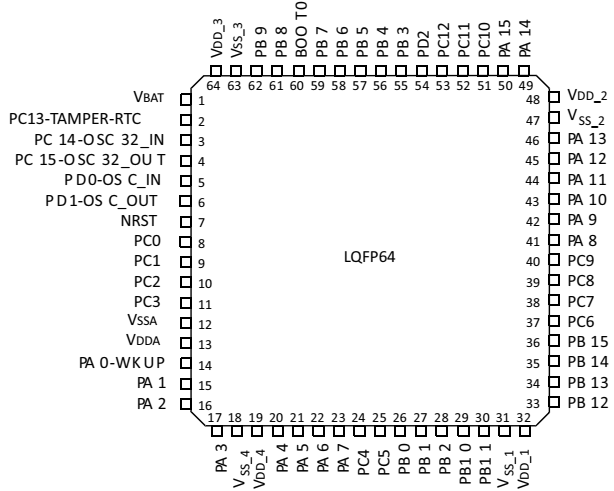
\includegraphics[scale=0.4]{image/hinh2_10}
    \end{center}
    \caption{Sơ đồ chân của dòng vi điều khiển STM32F103RCT6 64 chân \cite{9}}
    \label{refhinh2_10}
    \end{figure}
\section{Thiết bị giám sát các tham số môi trường nước BKRES}
Thiết bị giám sát tham số môi trường nước BKRES là sản phẩm của đề tài cấp Sở “NGHIÊN CỨU MÔ HÌNH MẠNG CẢM BIẾN KHÔNG DÂY GIÁM SÁT MÔI TRƯỜNG NƯỚC PHỤC VỤ PHÁT TRIỂN NUÔI TÔM CHÂN TRẮNG TẠI QUẢNG NINH” do thầy giáo TS. Nguyễn Hữu Phát làm chủ nhiệm. Đây là hệ thống cảm biến tự động thu thập dữ liệu về môi trường nước nặm của hồ nuôi trồng thủy sản và cảnh báo kịp thời khi có dấu hiệu bất thường trong môi trường nước.
\par 
Hệ thống tích hợp nhiều loại cảm biến, có thể đo đồng thời nhiều thông số của nước cùng lúc, cảnh báo tại chỗ mỗi khi các thông số vượt ngưỡng an toàn, kết hợp với trung tâm dữ liệu tập hợp, phân tích và dự đoán khả năng có thể xảy ra.
\par 
Các chức năng chính của hệ thống BKRES gồm có:
\begin{itemize}
\item Hệ thống đo đạc được 7 thông số môi trường nước (với thông số chu kỳ thời gian cho trước) bao gồm:
	\begin{itemize}
	\item Bốn thông số được đo trực tiếp (sử dụng cảm biến) gồm có:
 		\begin{itemize}
		\item	Hàm lượng Oxy trong nước,
		\item   Độ pH,
		\item	Nhiệt độ,
		\item	Nồng độ muối.
		\end{itemize}
	\item Ba thông số nội suy (tính toán từ các thông số đã đo được qua cảm biến):
 		\begin{itemize}
		\item	Nồng độ $NH_3$,
		\item	Nồng độ $H_2S$,
		\item	Nồng độ $NO_2$.
 		\end{itemize}
 	\end{itemize}
\item Hiển thị tại chỗ các thông số đo được lên LCD,
\item Cảnh báo cho người dùng khi các thông số vượt quá ngưỡng an toàn qua còi, đèn và qua SMS,
\item Lưu cấu hình vào bộ nhớ Flash để có thể phục hồi cấu hình khi bị mất điện,
\item Lưu lại nhật ký hệ thống vào thẻ nhớ (Có tùy chọn Bật/Tắt),
\item Mã hóa rồi gửi dữ liệu về máy chủ thông qua mạng di động,
\item Có khả năng điều chỉnh các thông số hệ thống từ xa qua máy chủ hoặc SMS (có mật khẩu),
\item Chu kỳ lấy dữ liệu, gửi dữ liệu về máy chủ, chu kỳ lưu giữ vào thẻ nhớ,
\item Cập nhật giá trị ngưỡng trên và dưới của thông số (Cho phép tự động cập nhật từ máy chủ),
\item Truy vấn thông tin hệ thống gồm các thông số cấu hình và tình trạng hệ thống,
\item Cập nhật và bảo trì hệ thống.
\end{itemize}
\par 
Yêu cầu khoa học cần đạt:
	\begin{itemize}
	\item Module phần cứng hoạt động ổn định trong môi trường khắc nghiệt, dễ dàng mở rộng, nâng cấp khi cần,
	\item Xử lý các dữ liệu từ cảm biến với tốc độ nhanh, tiêu tốn ít tài nguyên hệ thống nhất,
	\item Đảm bảo các phép tính toán có sai số ít nhất,
	\item Đảm bảo truyền thông tin cậy,
	\item Kích thước nhỏ gọn, tiêu thụ năng lượng thấp.
	\end{itemize}
\begin{figure}[h]
    \begin{center}
     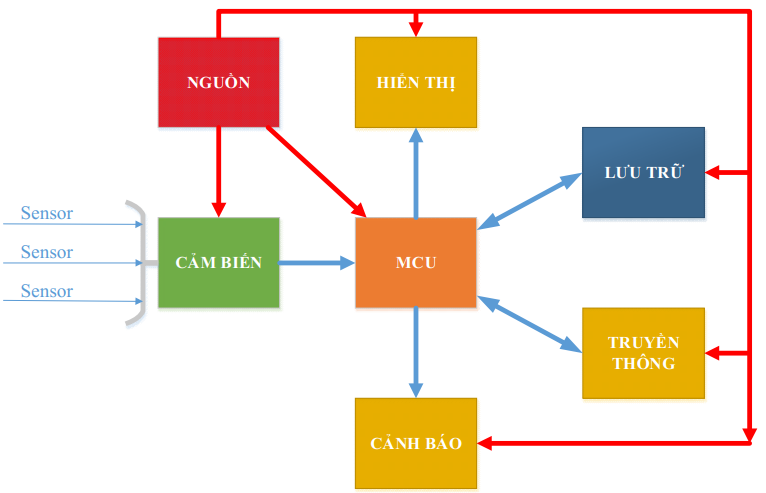
\includegraphics[scale=0.5]{image/hinh2_12}
    \end{center}
    \caption{Sơ đồ khối một thiết bị BKRES (client)}
    \label{refhinh2_12}
    \end{figure}
\par 
Máy chủ và thiết bị trao đổi dữ liệu qua việc trao đổi bản tin trên hạ tầng mạng GSM sử dụng giao thức TCP/IP nhằm đảm bảo dữ liệu truyền tải được chính xác và đầy đủ. Để máy chủ có thể nhận diện và giải mã dữ liệu được gửi đến thì phần dấu hiệu nhận diện bản tin và giá trị chỉ định kích thước bản tin cần được giữ nguyên không được mã hóa. Phần dữ liệu mã hóa chỉ bao gồm nội dung bản tin. Do đó, cấu trúc bản tin (Bảng 2.3) được xây dựng gồm có:
\begin{itemize}
\item HEADER: phần đầu bản tin và kích thước của toàn bộ bản tin,
\item Phần nội dung bản tin (phần được mã hóa) bao gồm:
  	\begin{itemize}
  	\item	Thông tin về ClientID,
  	\item	Loại bản tin (CommandID),
  	\item	Thông tin về thời gian (Timestamp),
  	\item 	Dữ liệu bản tin (Payload).
	\end{itemize}   
\item END: nhận diện kết thúc bản tin.
\end{itemize}
Nội dung bản tin xác thực gồm:
\begin{itemize}
\item Thông tin về phiên bản hệ thống,
\item Mã CODE (một thành phần tạo khóa AES),
\item Mã B (một thành phần tạo khóa AES),
\item Checksum.
\end{itemize}
Nội dung bản tin dữ liệu gồm:
\begin{itemize}
\item Thông tin về dữ liệu cảm biến: pH, Oxy, Salt, Temp, NH3, H2S,
\item Checksum.
\end{itemize} 
\begin{figure}[h]
    \begin{center}
     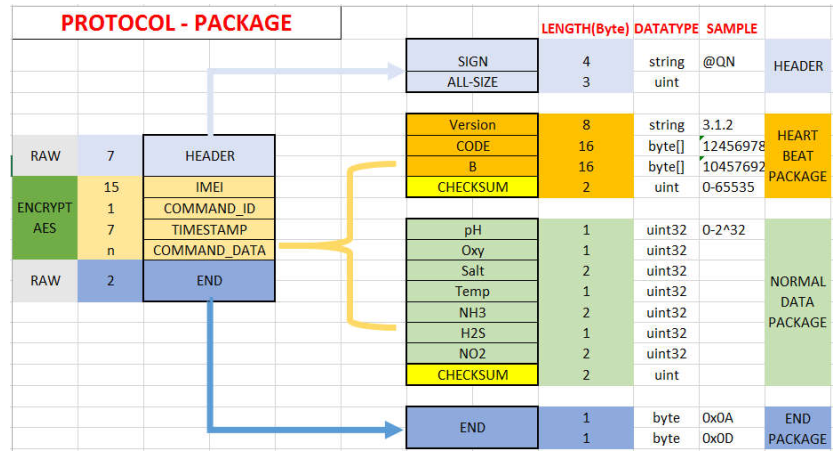
\includegraphics[scale=0.5]{image/hinh2_13}
    \end{center}
    \caption{Cấu trúc bản tin gửi dữ liệu trao đổi giữa máy chủ và client}
    \label{refhinh2_13}
\end{figure}
\par 
Hệ thống BKRES, sử dụng phương pháp truyền thông qua hệ thống GSM. Với việc sử dụng phương pháp này, mỗi thiết bị trong mạng cần phải có một module sim để truyền dữ liệu cho server, bên cạnh đó cần phải tốn chi phí hàng tháng để duy trì dịch vụ cho mỗi thiết bị. Phương pháp này có một số nhược điểm lớn là yêu cầu về cơ sở hạ tầng cao (cần có hệ thống GSM), khi hệ thống BKRES mở rộng (số lượng thiết bị lớn hơn) thì yêu cầu chi phí về việc duy trì hệ thống là lớn. Do đó, hệ thống BKRES hướng đến việc sử dụng công nghệ truyền thông LoRa để thu thập dữ liệu.
\section{Một số công cụ hỗ trợ khác}
\subsection{Phần mềm hỗ trợ cấu trình vi điều khiển}
Để cấu hình chức năng phần cứng cho các dòng vi điều khiển, ST đưa ra bộ công cụ STM32CubeMX \cite{10}. Phần mềm này hỗ trợ cấu hình các chức năng cho một vi điều khiển, phục vụ cho một dự án mới một cách trực quan, nhanh chóng. Ngoài ra, STM32CubeMX tự động download các driver mới nhất của ST dành cho các dòng chip của mình. Vì vậy đảm bảo các API của hãng sẽ luôn được cập nhật. Công cụ này còn hỗ trợ tự động sinh project mới với tùy chọn các IDE thông dụng. Giao diện phần mềm và giao diện cấu hình cho từng ngoại vi được thể hiện trong Hình \ref{refhinh2_14} và Hình \ref{refhinh2_15}{}.\\
\begin{figure}[h]
    \begin{center}
     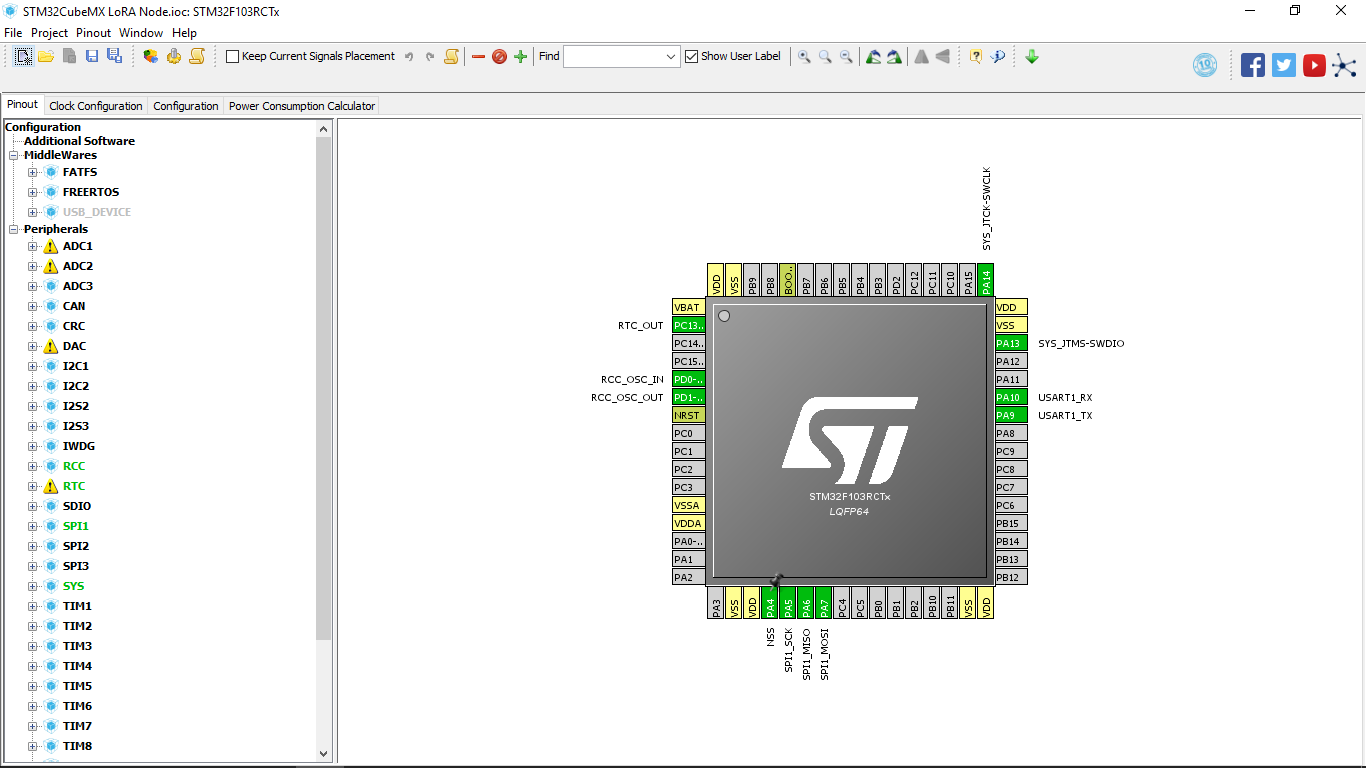
\includegraphics[scale=0.24]{image/hinh2_14}
    \end{center}
    \caption{Giao diện phần mềm STM32CubeMX hỗ trợ cấu hình}
    \label{refhinh2_14}
   \begin{center}
     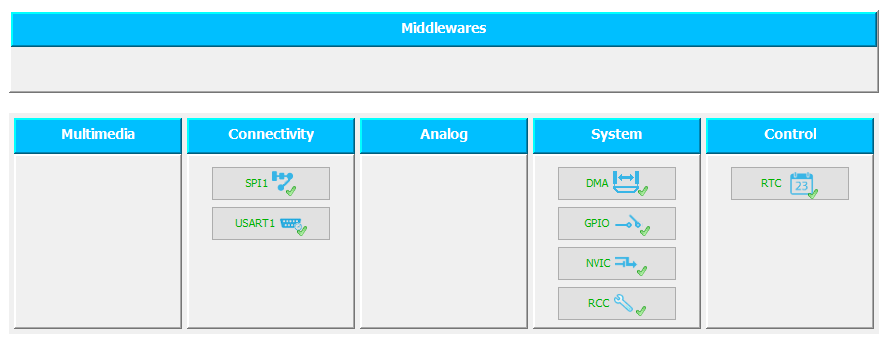
\includegraphics[scale=0.48]{image/hinh2_15}
    \end{center}
    \caption{Giao diện cấu hình chi tiết cho từng ngoại vi của STM32CubeMX}
    \label{refhinh2_15}
\end{figure}
\subsection{Phần mềm lập trình và biên dịch firmware Keil C}	
Keil C $\mu$Vision (Hình \ref{refhinh2_16}{}) là công cụ chuyên dụng hỗ trợ lập trình nhúng rất nổi tiếng. Keil C hỗ trợ hầu hết các loại chip vi xử lý trên thị trường và hỗ trợ 2 loại ngôn ngữ C/C++, Assembly. Nó được coi là IDE (môi trường phát triển) khá toàn diện, bao gồm khả năng biên dịch với trình biên dịch thương mại được tối ưu hóa, hỗ trợ nạp code và gỡ lỗi chuyên nghiệp.
\begin{figure}[h]
    \centering
     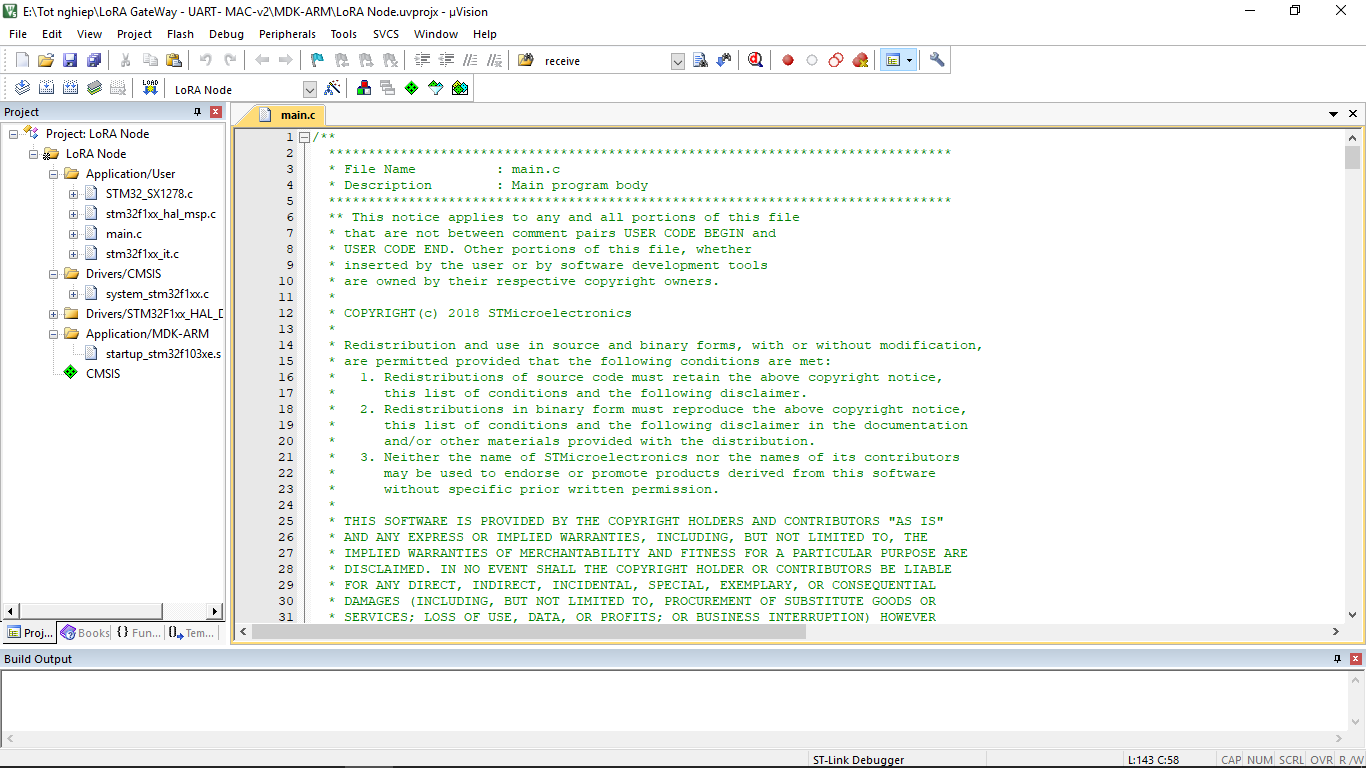
\includegraphics[scale=0.28]{image/hinh2_16}
    \caption{Giao diện phần mềm lập trình firmware Keil C $\mu$Vision}
    \label{refhinh2_16}
\end{figure}
\subsection{Phần mềm hỗ trợ giao tiếp UART Hercules} 
Trong quá trình lập trình, ngoài tính năng debug do phần mềm lập trình Keil C hỗ trợ, em còn sử dụng phần mềm Hercules (Hình \ref{refhinh2_17}{}) để hỗ trợ cho công việc kiểm tra và sửa lỗi. Hercules là một phần mềm hỗ trợ giao tiếp UART giúp hiển thị thông báo từ vi điều khiển lên máy tính, sử dụng đơn giản và thân thiện với người dùng. Sau khi kit kết nối với máy tính qua cổng COM, ta chỉ cần chọn đúng cổng COM được kết nối, chọn baud rate trùng với baud rate được cài đặt ở vi điều khiển, thế là có thể xem được thông báo từ vi điều khiển.\\
\begin{figure}[h]
\centering
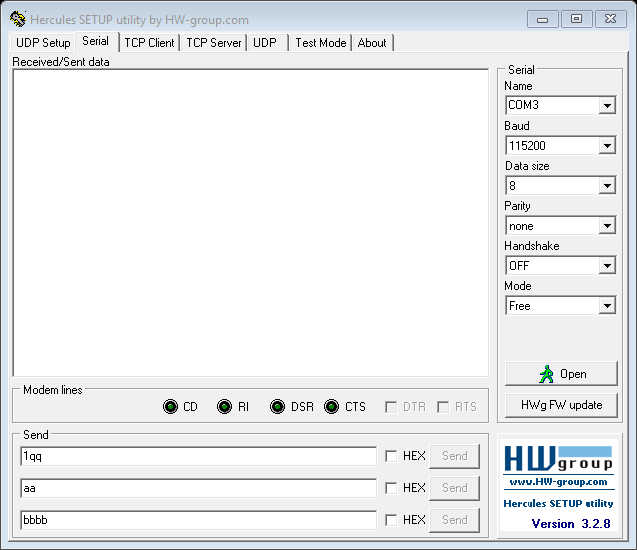
\includegraphics[scale=0.5]{image/hinh2_17}
\caption{Giao diện phần mềm HERCULES}
\label{refhinh2_17}
\end{figure}
\section{Kết luận}	
Từ những kiến thức em đã tìm hiểu và do những điểm phù hợp của ALOHA đối với hệ thống BKRES, em quyết định dựa trên giao thức ALOHA để xây dựng giao thức đa truy nhập và tích hợp giao thức đa truy nhập này vào thiết bị BKRES. Các bước tiến hành xây dựng giao thức sẽ được trình bày trong chương sau.







%\chapter{KIẾN TRÚC HỆ THỐNG}
\label{chapter3}
Từ những cơ sở lý thuyết thu thập ở chương 2, chương này em sẽ trình bày những bước giải quyết bài toán mà đề tài đưa ra.
\section{Phân tích yêu cầu}
Từ yêu cầu của đề tài và việc phân tích chi tiết yêu cầu và chức năng của hệ thống cần phải đáp ứng, em đã xác định được yêu cầu chức năng và phi chức năng của hệ thống như sau:
\begin{itemize}
\item	Yêu cầu chức năng:
	\begin{itemize}
	\item	Các nút truyền dữ liệu đến được Gateway,
	\item	Mạng có linh động về số lượng nút,
	\item	Số lượng nút trong mạng từ 3 nút trở lên.
	\end{itemize}
\item Yêu cầu phi chức năng:  
	\begin{itemize}
	\item 	Các nút truyền dữ liệu chính xác, ổn định,
	\item 	Nút tiêu tốn ít năng lượng,
	\item	Thiết bị hoạt động ổn định,
	\item	Hình thức gọn, phù hợp điều kiện làm việc.
	\item	Dữ liệu được đảm bảo an toàn,
	\item	Chi phí hợp lý.
	\end{itemize}
\end{itemize}
\section{Kiến trúc tổng thể hệ thống}
Dựa trên cơ sở kiến trúc đã có sẵn của thiết bị BKRES, hệ thống sẽ được tích hợp thêm module truyền thông LoRa vào các thiết bị của hệ thống. Khi đó hệ thống gồm 4 phân hệ chính. Hình \ref{construction}{} mô tỏ rõ hơn kiến trúc hệ thống.
\begin{itemize}
	\item Phân hệ cảm biến và xử lý dữ liệu: Ở mỗi nút mạng được trang bị các bộ cảm biến ghi đo 4 tham số (hàm lượng Oxy, nhiệt độ, độ pH và nồng độ muối). Dữ liệu cảm biến được gửi đến bộ điều khiển trung tâm (sử dụng vi điều khiển STM32) để xử lý, phân tích, đóng gói và gửi đến module truyền thông LoRa.
	\item Phân hệ truyền thông sử dụng LoRa: hoạt động theo mô hình đơn chặng, có nhiệm vụ gửi dữ liệu từ phân hệ cảm biến tới server trung tâm.
	\item Phân hệ cung cấp dịch vụ: Sau khi nhận dữ liệu từ phân hệ truyền thông, phân hệ này có nhiệm vụ xử lý dữ liệu và cung cấp các dịch vụ cho phân hệ giám sát và người dùng.
	\item Phân hệ giám sát và điều khiển: có nhiệm vụ hiển thị dữ liệu cảm biến một cách trực quan thông qua ứng dụng di động, ứng dụng web. Người dùng có thể cấu hình hệ thống, đặt các mức ngưỡng cảnh báo,… trên ứng dụng.
\end{itemize}
\begin{center}
\begin{figure}
\begin{center}
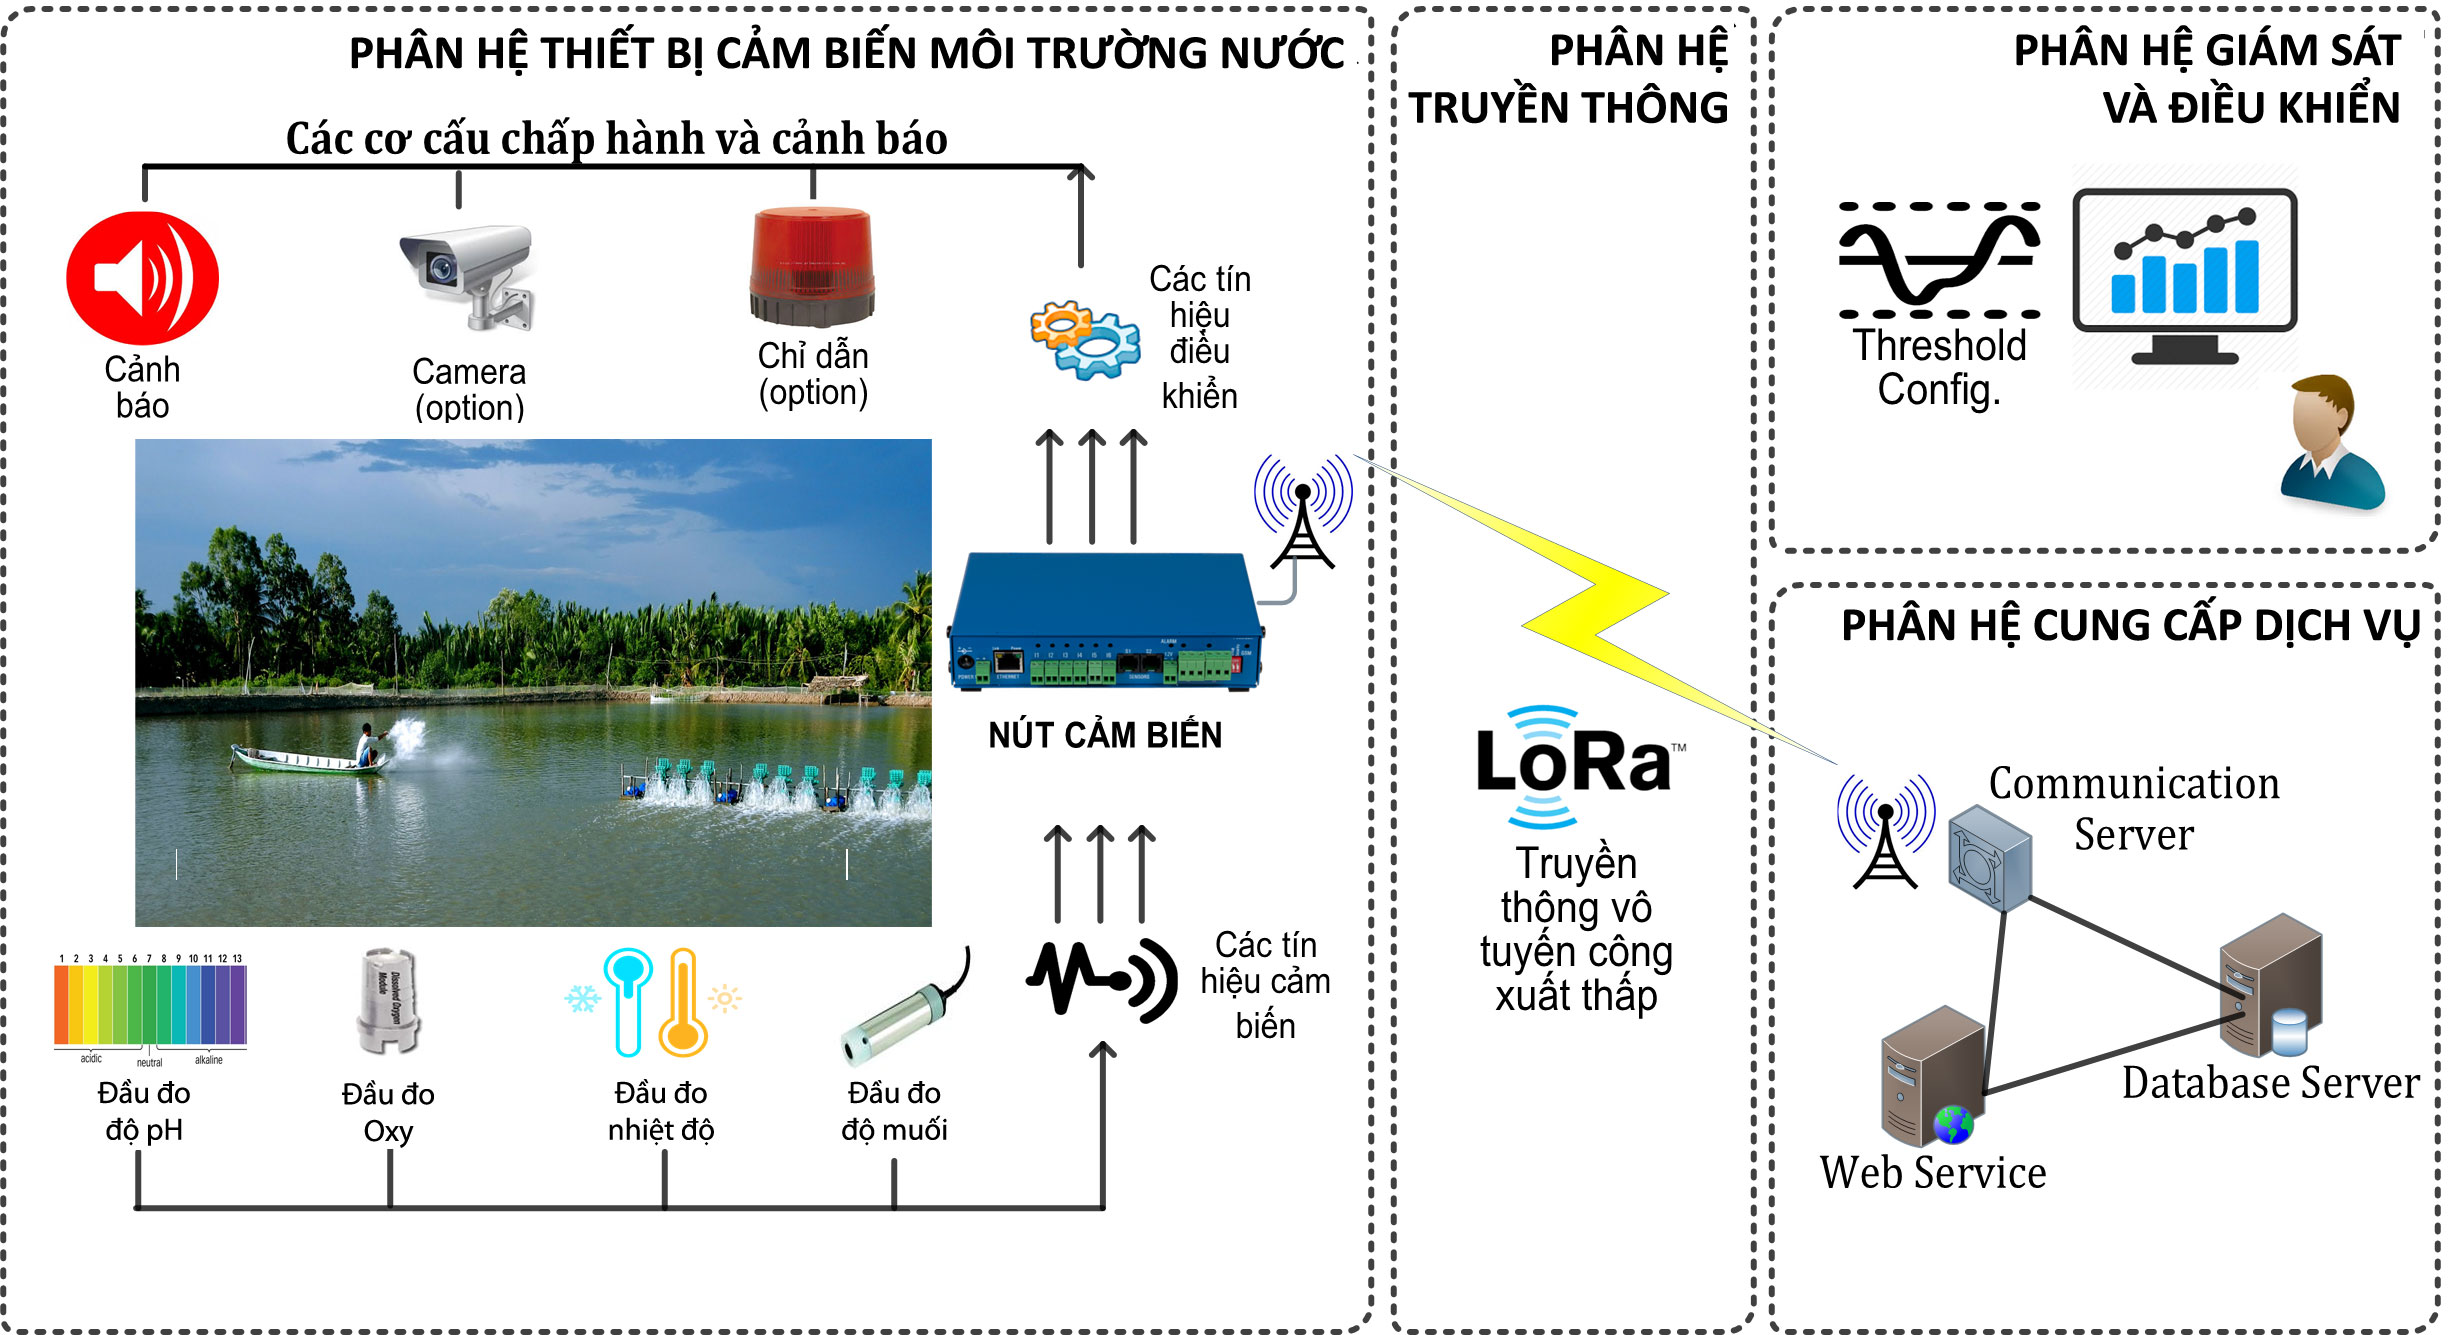
\includegraphics[scale=0.15]{image/kientrucLoRa}
\end{center}
\caption{Kiến trúc hệ thống}
\label{construction}
\end{figure}
\end{center}
\par 
Module LoRa SX1278 được lựa chọn để tích hợp vào thiết bị cảm biến như thể hiện trên hình \ref{moduleSX1278}{}. Nút cảm biến được thiết kế và chế tạo tài phòng nghiên cứu SANSLAB, gồm các thành phần phần cứng chính như: phân hệ cảm biến các tham số môi trường nước, phân hệ truyền thông, phân hệ vi xử lý và điều khiển, phân hệ cấp nguồn và phân hệ hiển thị, cảnh tại chỗ. Phần mềm trên nút cảm biến gồm firmware và drivers điều khiển hoạt động các phân hệ và ngoại vi, thuật toán đa truy nhập cũng được nhúng trong firmware của thiết bị. Một số thuật toán chính được biểu diễn qua các lưu đồ sau đây.
\section{Thiết kế nút mạng cảm biến tích hợp~module SX1278}
%\begin{center}
\begin{figure}[h]
	\begin{center}
		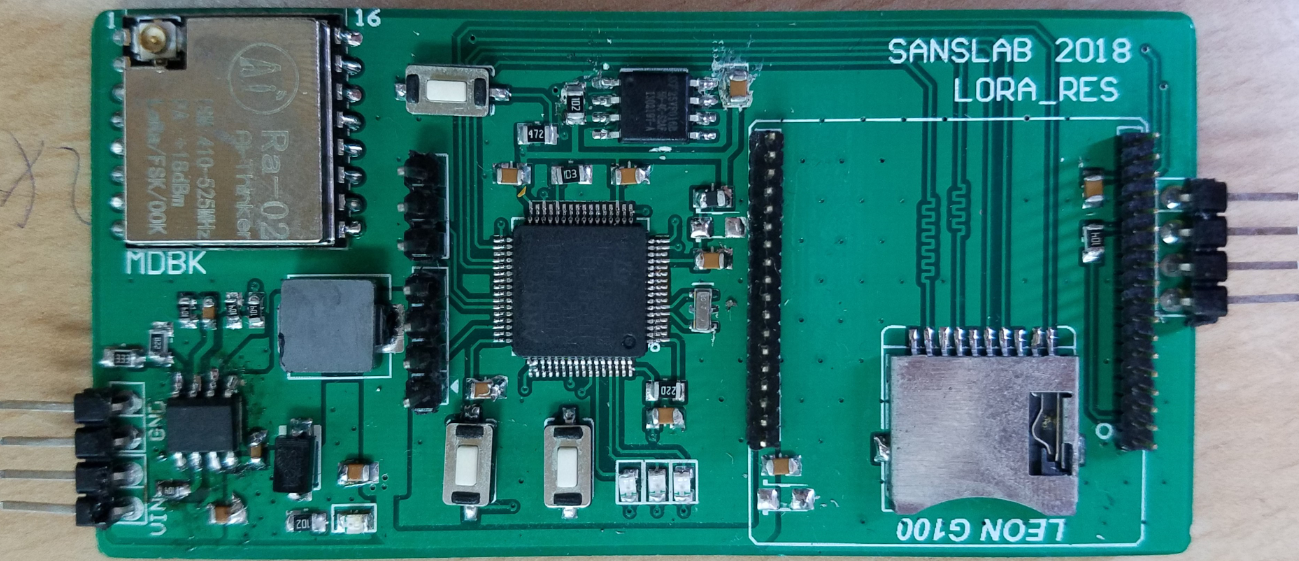
\includegraphics[scale=0.45]{image/hinh3_1}
	\end{center}
	\caption{Nút cảm biến tích hợp chip LoRa SX1278}
	\label{moduleSX1278}
\end{figure}
%\end{center}
\section{Mô hình mạng hình sao}
Thuật toán đa truy nhập đề xuất được phát triển và thử nghiệm trên mô hình gồm 3 nút cảm biến và một Gateway như hình \ref{protocol}{}. Để đánh giá khả năng truyền dữ liệu, độ ổn định, khả năng tùy biến và tự cấu hình của các nút trong mạng, em cấu hình các thông số cơ bản của các nút theo như bảng \ref{bang3_1}{}.
\begin{table}[h]
	\tabcolsep = 2cm
    \centering
    \caption{Bảng thông số cấu hình của các nút trong mạng}
    \begin{tabular}{|c|c|}
     	\hline
     	Thông số & Giá trị  \\
     	\hline
     	Channel & 11 (433 MHz)\\
     	\hline
     	BW & 125 kHz\\
     	\hline
     	CR & 4/5\\
     	\hline
     	SF & 7\\
     	\hline
     	Header & ON\\
     	\hline
     	CRC & ON\\
     	\hline
    \end{tabular}
    \label{bang3_1}
\end{table}
\par 
Khi mô hình hoạt động bình thường (hình \ref{normal}{}), 3 nút sẽ gửi dữ liệu đến Gateway theo một chu kỳ định sẵn. Trong thí nghiệm để kiếm tra sự ổn định của mạng một số thông số khoảng các của các nút với Gateway sẽ được thay đổi.\\
\begin{center}
\begin{figure}[h]
	\begin{center}
		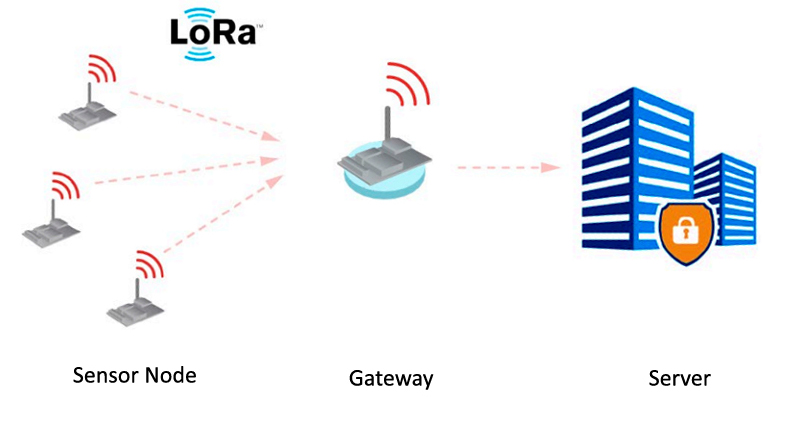
\includegraphics[scale=0.35]{image/normal}
	\end{center}
	\caption{Mô hình hoạt động của mạng}
	\label{normal}
\end{figure}
\end{center}
\par 
Trong trường hợp mạng đang hoạt động bình thường, có một nút mới tham gia vào mạng, nút này sẽ gửi yêu cầu đến Gateway. Sau khi được Gateway chấp nhận thì nút sẽ gửi dữ liệu đến Gateway theo một chu kỳ như những nút khác.
\section{Xây dựng lưu đồ thuật toán xử lý trên STM32}   
Với mô hình truyền thông hình sao như đề xuất trên, module truyền thông SX1278 trên mỗi nút mạng trong hệ thống được điều khiển bởi vi xử lý STM32 thông qua giao tiếp UART. Một số thuật toán điều khiển hoạt động của nút được trình bày trong các phần sau đây. 
\subsection{Gateway} 
 Trong quá trình truyền nhận dữ liệu, Gateway có các chức năng chính sau:
 \begin{itemize}
 \item	Gateway tự động cấu hình,
 \item	Nhận dữ liệu từ các nút,
 \item	Quản lý nút trong mạng.
 \end{itemize}
 \par 
Sau khi đã cấu hình cho gateway, trong vòng lặp vô hạn, gateway liên tục mở kênh truyền để nhận bản tin. Nếu bản tin đó là do một nút mới gửi đến (nút chưa tham gia vào mạng) thì gateway sẽ tiến hành quá trình xác thực nút. Còn nếu bản tin là bản tin chứa dữ liệu, Gateway sẽ nhận và xử lý dữ liệu và tiếp tục quá trình mở kênh truyền để nhận dữ liệu. Thuật toán \ref{gateway} thể hiện thuật toán xử lý của Gateway.
\begin{center}
\begin{algorithm}[h]
	\caption{Thuật toán của Gateway}
	\label{gateway}
	\begin{algorithmic}[1]
		\State $pass \gets sanslab$
		\State Gateway tự động cấu hình  \Comment{Gateway sẽ tự động cài một số thông số như ID, SF, CR, tần số,...}
		\While{1}
			\If{Nhận được gói tin}
				\State $packet \gets packet\_receive$	\Comment{gói tin nhận được}
				\If{$packet$ là gói tin gửi dữ liệu}
					\State $data \gets packet.data$
					\State Xử lý dữ liệu	\Comment{Gateway có thể gửi dữ liệu lên Server, hiển thị hoặc lưu dữ liệu}
				\ElsIf{$packet$ là gói tin yêu cầu tham gia mạng}
					\State	$ID \gets packet.src$	\Comment{Lấy ID của nút gửi đến}
					\State	$authentication \gets packet.data$ \Comment{Lấy dữ liệu bản tin xác thực}
					\State 	$response \gets true$
					\If{$authentication \neq pass$ }
						\State $response \gets flase$
					\EndIf
					\State gửi bản tin phản hồi response cho nút ID
				\EndIf
			\EndIf		
		\EndWhile
	\end{algorithmic}
\end{algorithm}
\end{center}
\subsection{Nút} 
Trong quá trình truyền nhận dữ liệu, nút có các chức năng chính sau:
\begin{itemize}
\item	Nút tự động cấu hình, mỗi nút có một ID khác nhau,
\item	Khi nút chưa tham gia mạng, nút sẽ gửi yêu cầu để tham gia mạng. Khi đó xảy ra một số trường hợp sau:
	\begin{itemize}
	\item	Quá trình yêu cầu không thành công, nút sẽ gửi lại,
	\item	Nếu bản tin xác thực sai, nút sẽ không hoạt động nữa,
	\item	Nếu quá trình yêu cầu tham gia mạng thành công, nút sẽ gửi dữ liệu.
	\end{itemize}
\item	Sau khi tham gia mạng thành công, nút sẽ gửi dữ liệu theo chu kỳ.
\end{itemize}
Sau khi được cấu hình, nút sẽ gửi bản tin xác thực cho Gateway (ID của Gateway được cấu hình sẵn trong nút). Nút sẽ thực hiện quá trình yêu cầu tham gia mạng (\ref{RequestJoinNetworks}) đến khi thành công (nếu bản tin xác thực sai, nút sẽ dừng lại). Sau khi nút nhận được bản tin chấp nhận tham gia vào mạng của Gateway, nút sẽ tiến hành quá trình gửi dữ liệu (quá trình này được thực hiên theo chu kỳ). Quá trình xử lý của nút được thể hiện \ref{node}{}.
\begin{center}
\begin{algorithm}[h]
	\caption{Thuật toán của Nút}
	\label{node}
	\begin{algorithmic}[1]
		\State {$msgAuthentication \gets sanslab$}
		\State Nút tự động cấu hình  \Comment{Nút sẽ tự động cài một số thông số như ID, SF, CR, tần số,...}
		
		\State {$idGateway \gets$ Địa chỉ Gateway}		
		\State {$response \gets 2 $} \Comment{response = 0 --> bản tin xác thực chính xác; response = 1 --> bản tin xác thực không chính xác; response = 2 --> nút chưa tham gia mạng}
		
		\State $RequestJoinNetworks(idGateway, msgAuthentication)$
		
		\While{1}
			\If{$response == 0$}
				\State $data \gets$ lấy dữ liệu từ cảm biến
				\State $cnt = 0$
				\Repeat
					\State $state \gets sendPacket(idGateway, data)$ 
					\If{$state > 0$} 
						\State Delay()
					\EndIf
					\State $cnt \gets cnt + 1$
				\Until{$state > 0$ and $cnt < threshold$} \Comment{threshold là số lần gửi tối đa}
			\ElsIf{$response == 1$} 
				\State $Sleep()$ 
				\Else
					\State $RequestJoinNetworks(idGateway, msgAuthentication)$
				\EndIf
			%\EndIf
		\EndWhile
	\end{algorithmic}
\end{algorithm}
\end{center}
\par 
Trong quá trình yêu cầu tham gia vào mạng, nút sẽ gửi bản tin xác thực đến khi nào nhận lại được bản tin phản hồi của Gateway. Khi đó nút sẽ biết đươc mình đã được chấp thuận tham gia mạng hay chưa. Còn về phần Gateway, sau khi nhận được bản tin xác thực được gửi từ nút, Gateway sẽ kiểm tra bản tin xác thực đó có chính xác không. Kết quả của quá trình kiểm tra bản tin xác thực sẽ được Gateway gửi lại cho nút
\begin{algorithm}
\caption{RequestJoinNetworks}
\label{RequestJoinNetworks}
\begin{algorithmic}[1]
  \Procedure {RequestJoinNetworks}{$idGateway$, $msgAuthentication$}
	\Repeat
			\State $state \gets sendPacket(idGateway, msgAuthentication)$ 
			\Comment{state là trạng thái của quá trình gửi tin; state = 0 gửi bản tin thành công; state > 0 gửi bản tin chưa thành công}
			\If{$state > 0$} 
				\State Delay()
			\ElsIf{Nhận được bản tin hồi đáp từ Gateway}
				\State $response \gets packet\_receive.data$
				\If{$response$ không chính xác} 
					\State $state \gets 1$
				\EndIf
			\EndIf
	\Until{$state > 0$}
  \EndProcedure
\end{algorithmic}
\end{algorithm}
\section{Kết luận}
Trong chương 3, em đã trình bày mô tả giao thức đa truy nhập mà em đã xây dựng để giải quyết đề tài. Sau quá trình xây dựng, triển khai và thí nghiệm, em xin trình bày kết quả đạt được trong chương sau.




\chapter{Xây dựng thuật toán đa truy nhập}
\label{chapter3}
Từ những cơ sở lý thuyết thu thập ở chương 2, chương này em sẽ trình bày quá trình thiết kế thuật toán đa truy nhập để ứng dụng thuật toán vào hệ thống BKRES-LoRa.
\section{Phân tích yêu cầu bài toán đa truy nhập}
Từ việc phân tích chi tiết yêu cầu và chức năng của thuật toán đa truy nhập cần phải đáp ứng, em đã xác định được yêu cầu chức năng và phi chức năng của hệ thống như sau:
\begin{itemize}
\item	Yêu cầu chức năng:
	\begin{itemize}
	\item	Có khả năng đa truy nhập (n - 1), tức là nhiều nút sẽ gửi dữ liệu đến 1 Gateway,			    \item	Có khả năng xử lý bài toán join/disjoin mạng,
	\item	Hoạt động được với số lượng nút lớn,
	\end{itemize}
\item Yêu cầu phi chức năng:  
	\begin{itemize}
	\item 	Các nút truyền dữ liệu chính xác,
	\item 	Nút tiêu tốn ít năng lượng,
	\item	Thiết bị hoạt động ổn định với thuật toán,
	\end{itemize}
\end{itemize}
\section{Hệ thống BKRES-LoRa}
\subsection{Kiến trúc tổng thể hệ thống}
Hệ thống giám sát tham số môi trường nước BKRES sau khi được tích hợp thêm module truyền thông LoRa thì dữ liệu thu thập được từ các nút sẽ được gửi đến Gateway thông qua module truyền thông LoRa, còn Gateway sẽ giao tiếp với server thông qua một số giao thức như TCP/IP, GSM,...Hình \ref{construction}{} sẽ mô tả rõ hơn kiến trúc gồm 4 phân hệ chính của hệ thống BKRES-LoRa.
\begin{itemize}
	\item Phân hệ cảm biến và xử lý dữ liệu: Ở mỗi nút mạng được trang bị các bộ cảm biến ghi đo 4 tham số (hàm lượng Oxy, nhiệt độ, độ pH và nồng độ muối) để thu thập dữ liệu tham số môi trường. Dữ liệu cảm biến được gửi đến bộ điều khiển trung tâm (sử dụng vi điều khiển STM32) để phân tích, xử lý, đóng gói và gửi đến module truyền thông LoRa.
	\item Phân hệ truyền thông sử dụng LoRa: Hoạt động theo mô hình đơn chặng, có nhiệm vụ gửi dữ liệu từ phân hệ cảm biến đến Gateway và từ đó dữ liệu được gửi đến server trung tâm.
	\item Phân hệ cung cấp dịch vụ: Sau khi nhận dữ liệu từ phân hệ truyền thông, phân hệ này có nhiệm vụ xử lý dữ liệu và cung cấp các dịch vụ cho phân hệ giám sát và người dùng.
	\item Phân hệ giám sát và điều khiển: có nhiệm vụ hiển thị dữ liệu cảm biến một cách trực quan thông qua ứng dụng di động, ứng dụng web. Người dùng có thể cấu hình hệ thống, đặt các mức ngưỡng cảnh báo,… trên ứng dụng.
\end{itemize}
\begin{center}
\begin{figure}
\begin{center}
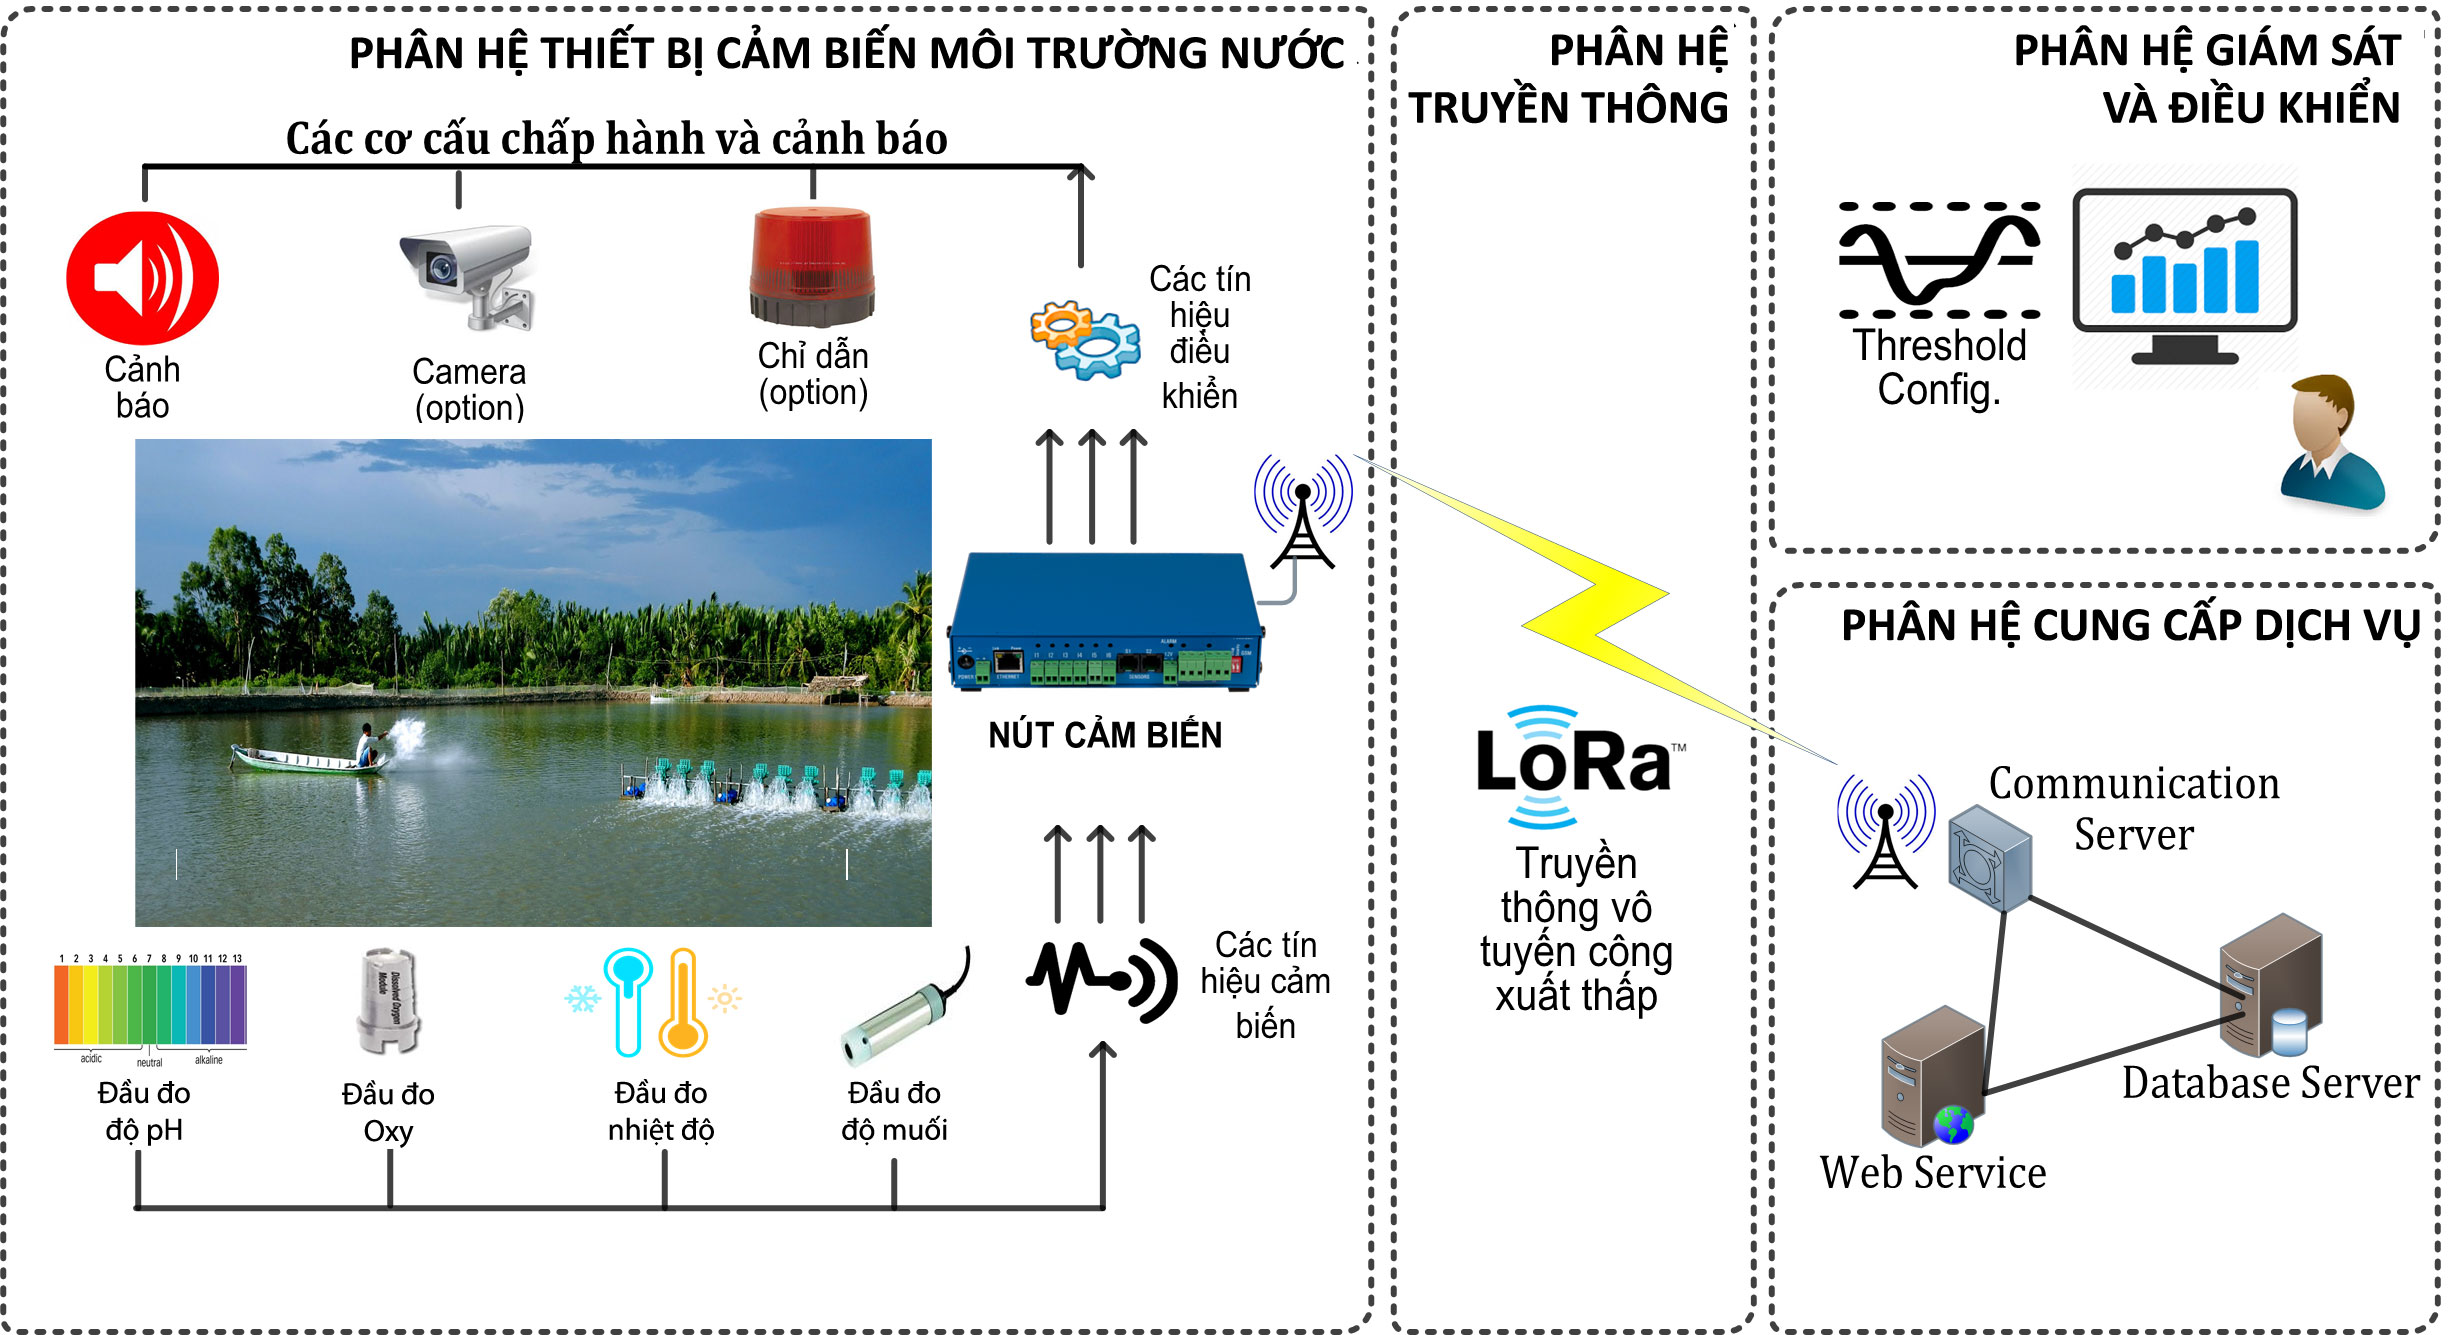
\includegraphics[scale=0.15]{image/kientrucLoRa}
\end{center}
\caption{Kiến trúc hệ thống}
\label{construction}
\end{figure}
\end{center}
\par Module LoRa SX1278 được lựa chọn để tích hợp vào thiết bị cảm biến như thể hiện trên Hình \ref{moduleSX1278}{}. Nút cảm biến được thiết kế và chế tạo tài phòng nghiên cứu SANSLAB, gồm các thành phần phần cứng chính như: phân hệ cảm biến các tham số môi trường nước, phân hệ truyền thông, phân hệ vi xử lý và điều khiển, phân hệ cấp nguồn và phân hệ hiển thị, cảnh tại chỗ. Phần mềm trên nút cảm biến gồm firmware và drivers điều khiển hoạt động các phân hệ và ngoại vi, thuật toán đa truy nhập cũng được nhúng trong firmware của thiết bị.
\subsection{Nút mạng cảm biến tích hợp module SX1278}
%\begin{center}
\begin{figure}[h]
	\begin{center}
		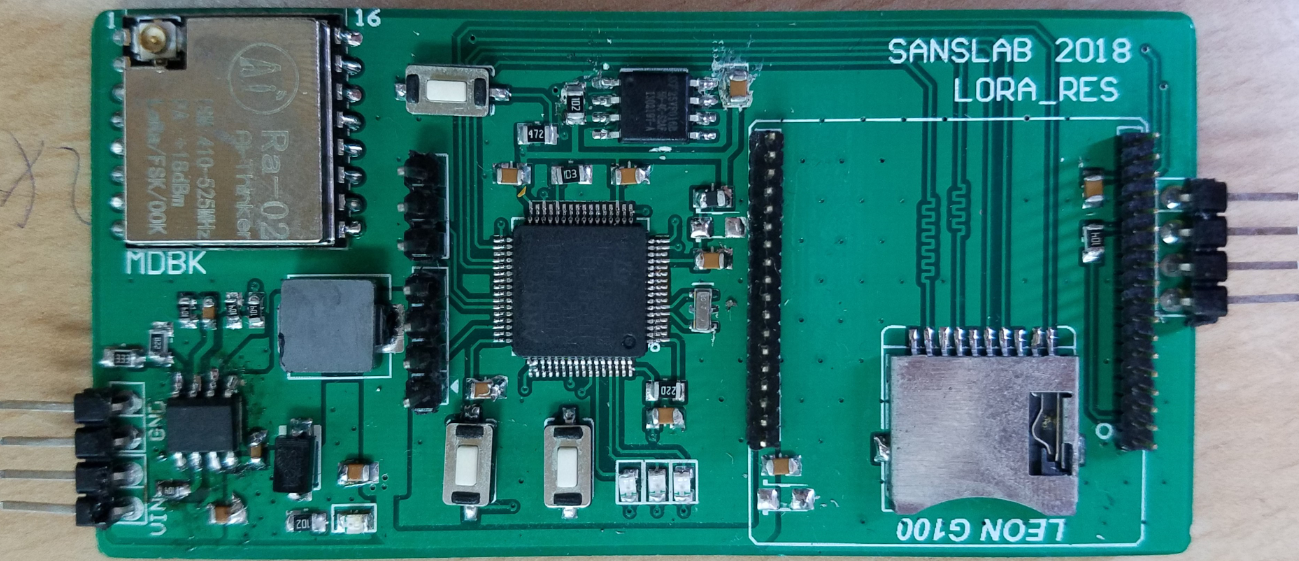
\includegraphics[scale=0.38]{image/hinh3_1}
	\end{center}
	\caption{Nút cảm biến tích hợp chip LoRa SX1278}
	\label{moduleSX1278}
\end{figure}
%\end{center}
\noindent Nút cảm biến được thiết kế gồm các khối có nhiệm vụ như sau:
\begin{itemize}
\item	Khối nguồn: có nhiệm vụ cung cấp nguồn cho toàn bộ mạch. Mức điện áp 3,3 V cung cấp cho vi điều khiển, thiết bị ngoại vi cùng với cảm biến. Nguồn cung cấp cho mạch là pin, nhỏ gọn và có thể sạc được nên rất phù hợp với các thiết bị trong mạng WSN,
\item	Khối xử lý trung tâm: có nhiệm vụ lấy dữ liệu từ các thiết bị cảm biến, xử lý rồi chuyển qua khối truyền thông, cũng như xử lý các thông tin nhận được từ khối truyền thông. Khối xử lý trung tâm sử dụng vi điều khiển STM32F1 là một loại vi điều khiển lõi Cortex M3 có tốc độ xử lý cao, cấu hình mạnh, tiết kiệm năng lượng với kích thước nhỏ gọn và giá thành rẻ,
\item	Khối truyền thông: có nhiệm vụ truyền nhận dữ liệu giữa các thiết bị trong mạng. Khối truyền thông sử dụng module LoRa Ai Thinker SX1278 được kết nối với khối xử lý trung tâm qua giao tiết SPI,
\item	Khối lưu trữ dữ liệu: được dùng để lưu trữ cấu hình hệ thống cùng với nhật ký cảm biến. Khối này gồm IC flash NAND SST25VF016B và thẻ nhớ. IC flash có tốc độ xử lý cao, dung lượng bộ nhớ nhỏ thích hợp với việc lưu trữ phần mềm cùng với cấu hình của hệ thống. Thẻ nhớ được sử dụng để lưu trữ nhật ký cảm biến, dễ dàng cho người sử dụng có thể kiểm tra và sao lưu dữ liêu.
\end{itemize}
\subsection{Mô hình hoạt động của hệ thống BKRES-LoRa}
Thuật toán đa truy nhập đề xuất được phát triển và thử nghiệm trên mô hình gồm 3 nút cảm biến và một Gateway như Hình \ref{normal}{}. Để đánh giá khả năng truyền dữ liệu, độ ổn định, khả năng tùy biến và tự cấu hình của các nút trong mạng, các thông số cơ bản của các nút sẽ được thiết lập theo như Bảng \ref{bang3_1}{}.
\begin{table}[h]
	\tabcolsep = 2cm
    \centering
    \caption{Bảng thông số cấu hình của các nút trong mạng}
    \begin{tabular}{|c|c|}
     	\hline
     	Thông số & Giá trị  \\
     	\hline
     	Channel & 11 (433 MHz)\\
     	\hline
     	BW & 125 kHz\\
     	\hline
     	CR & 4/5\\
     	\hline
     	SF & 7\\
     	\hline
     	Header & ON\\
     	\hline
     	CRC & ON\\
     	\hline
    \end{tabular}
    \label{bang3_1}
\end{table}
\par 
Hoạt động của mô hình được mô tả như sau. Ban đầu, mỗi nút mới (sau khi tự động cấu hình) sẽ gửi yêu cầu tham gia mạng đến Gateway, sau khi được chấp nhận thì nút bắt đầu quá trình gửi dữ liệu đến Gateway. Trong quá trình này, mỗi nút sẽ nhận dữ liệu đã được xử lý từ vi điều khiển, rồi gửi dữ liệu đến Gateway theo một chu kỳ định sẵn. Trong trường hợp xảy ra lỗi với bộ truyền thông LoRa, nút sẽ gửi dữ liệu trực tiếp đến server trung tâm qua mạng GSM (có sẵn trong BKRES phiên bản cũ), đến khi hết xảy ra lỗi với bộ truyền thông, nút lại bắt đầu lại quá trình như bình thường.\\
\begin{figure}[h]
	\centering
		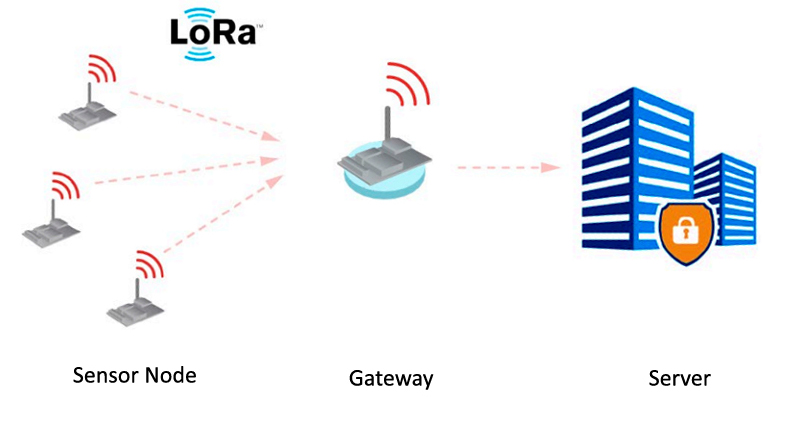
\includegraphics[scale=0.4]{image/normal}
	\caption{Mô hình hoạt động của mạng}
	\label{normal}
\end{figure}
\section{Xây dựng thuật toán đa truy nhập}
Do số lượng nút trong mạng ít, nên em quyết định sử dụng phương pháp đa truy nhập ngẫu nhiên, tức là khi nút có dữ liệu nó sẽ gửi luôn bản tin cho Gateway.
\subsection{Thuật toán đa truy nhập của Gateway}
Trong thuật toán đa truy nhập, Gateway có các nhiệm vụ chính sau:
 \begin{itemize}
 \item	Nhận dữ liệu từ các nút,
 \item	Quản lý nút trong mạng.
 \end{itemize}
 \par 
Sau khi đã tự cấu hình, trong vòng lặp vô hạn, Gateway liên tục mở kênh truyền để nhận bản tin. Nếu bản tin đó là do một nút mới gửi đến (nút chưa tham gia vào mạng) thì gateway sẽ tiến hành quá trình xác thực nút, rồi gửi bản tin phản hồi cho nút. Còn nếu bản tin là bản tin chứa dữ liệu, Gateway sẽ nhận và xử lý dữ liệu và tiếp tục quá trình mở kênh truyền để nhận dữ liệu. Algorithm \ref{gateway} thể hiện thuật toán xử lý của Gateway.
\begin{center}
\begin{algorithm}[h]
	\caption{Thuật toán của Gateway}
	\label{gateway}
	\begin{algorithmic}[1]
		\State $pass \gets @Rsanslab$
		\State Gateway tự động cấu hình  \Comment{Gateway sẽ tự động cài một số thông số như ID, SF, CR, tần số,...}
		\While{1}
			\If{Nhận được gói tin}
				\State $packet \gets packet\_receive$	\Comment{gói tin nhận được}
				\If{$packet$ là gói tin gửi dữ liệu}
					\State $data \gets packet.data$
					\State Xử lý dữ liệu	\Comment{Gateway có thể gửi dữ liệu lên Server, hiển thị hoặc lưu dữ liệu}
				\ElsIf{$packet$ là gói tin yêu cầu tham gia mạng}
					\State	$ID \gets packet.src$	\Comment{Lấy ID của nút gửi đến}
					\State	$authentication \gets packet.data$ \Comment{Lấy dữ liệu bản tin xác thực}
					\State 	$response \gets true$
					\If{$authentication \neq pass$ }
						\State $response \gets flase$
					\EndIf
					\State gửi bản tin phản hồi response cho nút ID
				\EndIf
			\EndIf		
		\EndWhile
	\end{algorithmic}
\end{algorithm}
\end{center}
\subsection{Thuật toán đa truy nhập của nút} 
Chức năng chính của nút trong thuật toán đa truy nhập:
\begin{itemize}
\item	Khi nút chưa tham gia mạng, nút sẽ gửi yêu cầu để tham gia mạng. Khi đó xảy ra một số trường hợp sau:
	\begin{itemize}
	\item	Quá trình yêu cầu không thành công, nút sẽ gửi lại,
	\item	Nếu bản tin xác thực sai, nút sẽ không hoạt động nữa,
	\item	Nếu quá trình yêu cầu tham gia mạng thành công, nút sẽ gửi dữ liệu.
	\end{itemize}
\item	Sau khi tham gia mạng thành công, nút sẽ gửi dữ liệu theo chu kỳ.
\end{itemize}
\begin{algorithm}[H]
	\caption{Thuật toán của Nút}
	\label{node}
	\begin{algorithmic}[1]
		\State {$msgAuthentication \gets @Rsanslab$}
		\State Nút tự động cấu hình  \Comment{Nút sẽ tự động cài một số thông số như ID, SF, CR, tần số,...}
		
		\State {$idGateway \gets$ Địa chỉ Gateway}		
		\State {$response \gets 2 $} \Comment{response = 0 --> bản tin xác thực chính xác; response = 1 --> bản tin xác thực không chính xác; response = 2 --> nút chưa tham gia mạng.}
		
		\State $RequestJoinNetworks(idGateway, msgAuthentication)$
		
		\While{1}
			\If{$response == 0$}
				\State $data \gets$ lấy dữ liệu từ cảm biến
				\State $cnt = 0$
				\Repeat
					\State $state \gets sendPacket(idGateway, data)$ 
					\If{$state > 0$} 
						\State $Delay()$
					\EndIf
					\State $cnt \gets cnt + 1$
				\Until{$state > 0$ and $cnt < threshold$} \Comment{threshold là số lần gửi tối đa}
			\ElsIf{$response == 1$} 
				\State $Sleep()$ 
				\Else
					\State $RequestJoinNetworks(idGateway, msgAuthentication)$
				\EndIf
			%\EndIf
		\EndWhile
	\end{algorithmic}
\end{algorithm}
Sau khi được cấu hình, nút sẽ gửi bản tin xác thực cho Gateway (ID của Gateway được thiết lập sẵn). Nút sẽ thực hiện quá trình yêu cầu tham gia mạng (quá trình yêu cầu tham gia mạng được mô tả bởi Algorithm \ref{RequestJoinNetworks}) đến khi thành công (nếu bản tin xác thực sai, nút sẽ dừng lại). Sau khi nút nhận được bản tin chấp nhận tham gia vào mạng của Gateway, nút sẽ tiến hành quá trình gửi dữ liệu. Quá trình xử lý của nút được thể hiện bởi Algorithm \ref{node}{}.
\par 
Trong quá trình yêu cầu tham gia vào mạng, nút sẽ gửi bản tin xác thực đến khi nào nhận lại được bản tin phản hồi của Gateway. Khi đó nút sẽ biết đươc mình đã được chấp thuận tham gia mạng hay chưa. Còn về phần Gateway, sau khi nhận được bản tin xác thực được gửi từ nút, Gateway sẽ kiểm tra bản tin xác thực đó có chính xác không. Kết quả của quá trình kiểm tra bản tin xác thực sẽ được Gateway gửi lại cho nút.
\begin{algorithm}[H]
\caption{RequestJoinNetworks}
\label{RequestJoinNetworks}
\begin{algorithmic}[1]
  \Procedure {RequestJoinNetworks}{$idGateway$, $msgAuthentication$}
	\Repeat
			\State $state \gets sendPacket(idGateway, msgAuthentication)$ 
			\Comment{state là trạng thái của quá trình gửi tin; state = 0 gửi bản tin thành công; state > 0 gửi bản tin chưa thành công}
			\If{$state > 0$} 
				\State Delay()
			\ElsIf{Nhận được bản tin hồi đáp từ Gateway}
				\State $response \gets packet\_receive.data$
				\If{$response$ không chính xác} 
					\State $state \gets 1$
				\EndIf
			\EndIf
	\Until{$state > 0$}
  \EndProcedure
\end{algorithmic}
\end{algorithm}
\section{Xây dựng chi tiết và đánh giá}
\subsection{Bản tin yêu cầu tham gia mạng}
Bản tin yêu cầu tham gia mạng sẽ được gửi khi nút đã tự cấu hình. Để giảm số lượng bản tin phải trao đổi giữa nút và Gateway để tham gia mạng, thì bản tin yêu cầu tham gia mạng sẽ chứa luôn bản tin xác thực. Trong quá trình thử nghiệm, chuỗi xác thực sẽ là "@Rsanslab" và được cấu hình sẵn trong firmware của cả nút và Gateway. Gateway sau khi nhận được bản tin yêu cầu tham gia mạng của nút, sẽ tách phần dữ liệu (chứa chuỗi xác thực) để so sánh với chuỗi xác thực của nó rồi tiến hành phản hồi cho nút. Cấu trúc gói yêu cầu tham gia mạng được mô tả trong bảng \ref{construction_rq}{}.
\begin{table}[h]
 \centering
    \caption{Cấu trúc bản tin yêu cầu tham gia mạng}
    \begin{tabular}{|c|c|}
    	\hline
     	Header & Data \\
     	\hline
     	2 byte & max. 255 byte\\
     	\hline
    \end{tabular}
    \label{construction_rq}
\end{table}
Trong thí nghiệm, bản tin yêu cầu tham gia mạng tương đối đơn giản mục đích để giảm thời gian xác thực của Gateway. Cấu trúc cụ thể bản tin:
\begin{itemize}
\item	Header: @R,
\item	Data: sanslab.
\end{itemize}
\par 
Luồng trao đổi bản tin giữa nút và Gateway sẽ được mô tả trong Hình \ref{refluong1}{}. Dữ liệu của bản tin phản hồi chỉ là "1" nếu bản tin xác thực chính xác hoặc là "0" nếu bản tin xác thực không chính xác.\\
\begin{figure}[h]
\begin{center}
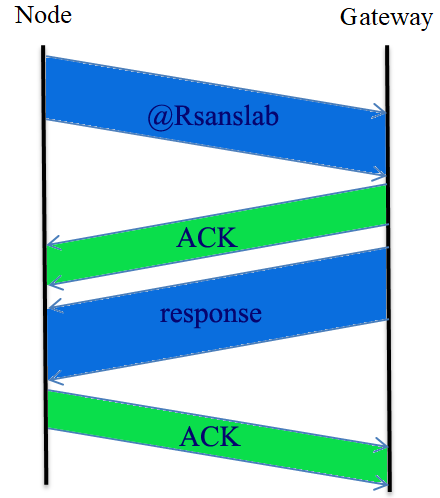
\includegraphics[scale= 0.5]{image/luong1}
\end{center}
\caption{Luồng trao đổi dữ liệu trong quá trình yêu cầu tham gia mạng}
\label{refluong1}
\end{figure}
\par 
Thuật toán yêu cầu tham gia mạng sẽ xảy ra 2 trường hợp:
\begin{itemize}
\item Trường hợp tốt nhất: Nút gửi yêu cầu tham gia mạng đến Gateway và nhận luôn được bản tin phải hồi của Gateway. Khi đó độ phức tạp của thuật toán là O(c).
\item Trường hợp xấu nhất: Nút gửi yêu cầu tham gia mạng đến Gateway nhưng không nhận được bản tin phản hồi của Gateway (hoặc gửi bản tin không thành công), nút sẽ gửi lại bản tin yêu cầu tham gia mạng. Khi đó độ phức tạp của thuật toán là O(n).
\end{itemize}
\subsection{Bản tin gửi dữ liệu}
Sau khi đã tham gia mạng thành công, theo chu kỳ, nút bắt đầu gửi bản tin chứa dữ liệu đến Gateway. Do số lượng nút nhỏ (3 đến 4 nút) nên khả năng xảy ra va chạm dẫn đến mất gói là rất ít. Do đó, nguyên nhân chính khiến nút gửi bản tin không thành công là do nút gửi bản tin không đúng vào thời điểm Gateway mở kênh truyền để nhận bản tin. Khi không gửi được bản tin thì nút sẽ trễ một khoảng thời gian, sau đó sẽ gửi lại bản tin. Cũng như bản tin yêu cầu tham gia mạng, bản tin chứa dữ liệu có phần header để nhận diện, ngoài ra bản tin còn chứa các thông số khác. Bản \ref{construction_data} mô tả cấu trúc bản tin gửi dữ liệu.\\
\begin{table}[h]
\centering
\caption{Cấu trúc bản tin dữ liệu}
	\begin{tabular}{|c|c|c|c|c|c|}
	\hline
	Header & IMEI & Command\_ID & Timestamp & Data & End \\
	\hline
	7 byte & 15 byte & 1 byte & 7 byte & max. 255 byte & 2 byte\\
	\hline 
	\end{tabular}
	\label{construction_data}
\end{table}\\
Luồng trao đổi bản tin dữ nút và Gateway được mô tả trong Hình \ref{senddata}{}.
\begin{figure}[htp]
\label{senddata}
\subfigure[Gửi bản tin thành công.]
  {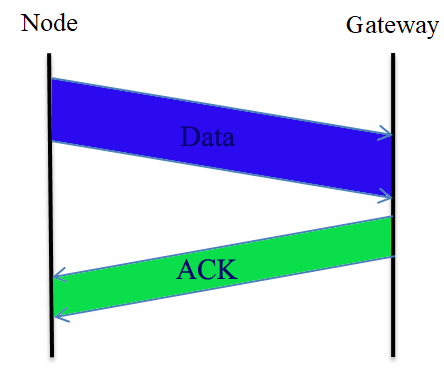
\includegraphics[width = .49\linewidth]{image/send_data}}\hfill
\subfigure[Gửi bản tin gặp xung đột và gửi lại.]
  {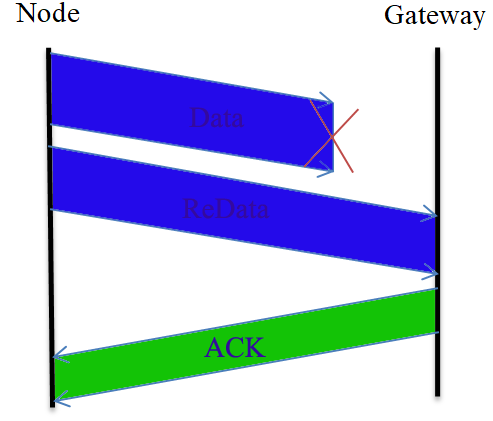
\includegraphics[width = .49\linewidth]{image/resend_data}}
  \caption{Luồng dữ liệu trong hai trường hợp}
\end{figure}
\begin{itemize}
\item Header: chứa dấu hiệu nhận diện bản tin chứa dữ liệu ("@DN") và kích thước của bản tin,
\item IMEI: là mã nhận dạng giữa các thiết bị với nhau, mỗi thiết bị có một IMEI khác nhau được cấu hình sẵn,
\item Command\_ID: là loại bản tin,
\item Timestamp: chứa thông tin về thời gian của dữ liệu (gồm: ngày, tháng, năm, giờ, phút, giây) được lấy từ vi điều khiển,
\item Data: chứa dữ liệu các thông số môi trường nước, gồm lần lượt các trường sau: pH, Oxy, Salt, Temp, $NH_3$, $H_2S$, $NO_2$,
\item End: báo hiệu kết thúc bản tin, là ký tự "\$".
\end{itemize}
Trong cả hai trường hợp gửi bản tin gặp xung đột và không gặp xung đột độ phức tạp của thuật toán là O(c) do số lần gửi lại của nút không được quá số lần quy định để đảm bảo tính thời gian thực của dữ liệu.
\section{Kết luận}
Sau khi đã xây dựng và đánh giá thuật toán đa truy nhập một cách kỹ lưỡng, thuật toán sẽ được triển khai dưới dạng code và nhúng vào những thiết bị trong hệ thống BKRES-LoRa. Quá trình thử nghiệm cùng với kết quả thử nghiệm sẽ được mô tả trong Chương \ref{chapter4}{}.





\chapter{Kết quả và đánh giá}
\label{chapter4}
Sau khi đã xây dựng thành công thuật toán đã trình bày trong 3, em tiến hành thực nghiệm để phát hiện và điều chỉnh để thuật toán đa truy nhập tốt hơn. Chương này, em xin trình bày về những kết quả đã đạt được và hướng phát triển của đề tài.
\section{Các kết quả đạt được}
\subsection{Phân tích kết quả các thử nghiệm}
Sau khi tự động cấu hình, nó sẽ gửi yêu cầu tham gia mạng đến Gateway và bắt đầu gửi tin (nếu được Gateway chấp thuận). Hình \ref{receivePacket} mô tả quá trình kiểm tra yêu cầu tham gia mạng của nút và nhận gói tin từ nút.
\begin{figure}[h]
\centering
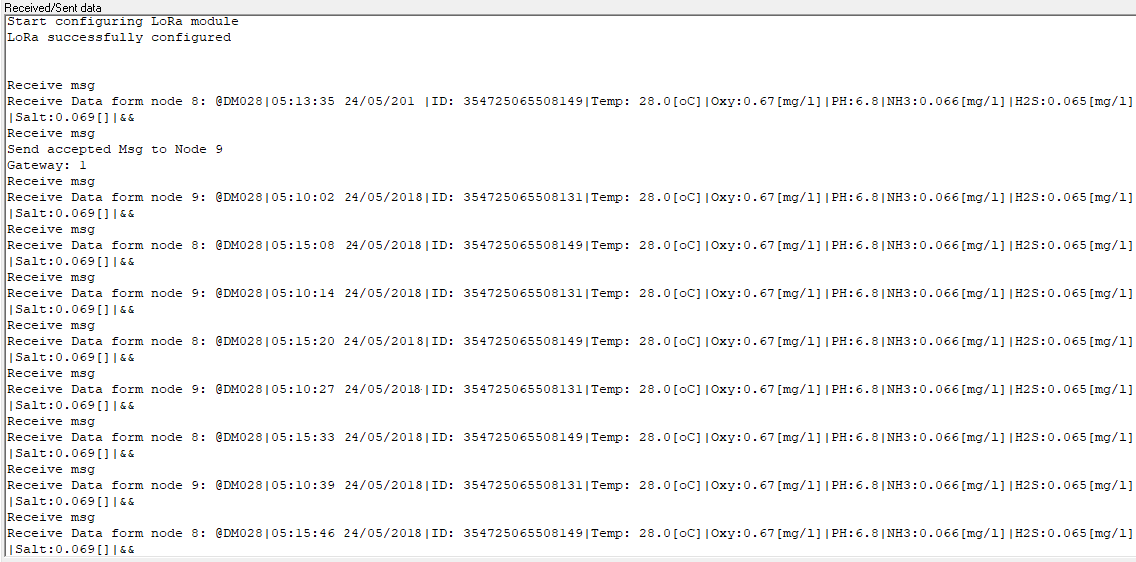
\includegraphics[scale=0.4]{image/receivePacket}
\caption{Quá trình xử lý của Gateway}
\label{receivePacket}
\end{figure}
\subsubsection{Thử nghiệm 1: Đánh giá mất gói trong điều kiện thuận lợi (PTN)}
Thử nghiệm này được triển khai tại phòng nghiên cứu Sanslab, thí nghiệm thực hiện gồm có 3 nút và 1 gateway. Các thông số kỹ thuật được cấu hình như trong Bảng \ref{bang3_1}, các nút nằm trong bán kính 10 m của Gateway. Ngoài ra có hai số thông số được thiết lập trước là ID của nút và ID của Gateway. Kết quả của thực nghiệm được mô tả trong Bảng \ref{TN1} và biểu đồ Hình \ref{sendrate}{}.\\
\begin{table}[h]
\centering
\caption{Bảng kết quả độ mất gói trong điều kiện thuận lợi}
\label{TN1}
\begin{tabular}{|c|c|c|c|}
\hline
 & Nút 2 & Nút 3 & Nút 4 \\
 \hline
 Gửi gói tin thành công & 98,77,02 \% & 98,98 \% & 100 \% \\
 \hline
 Hủy gói tin & 1,23 \% & 1,03 \% & 0 \% \\
 \hline
\end{tabular}
\end{table}
\begin{figure}
\centering
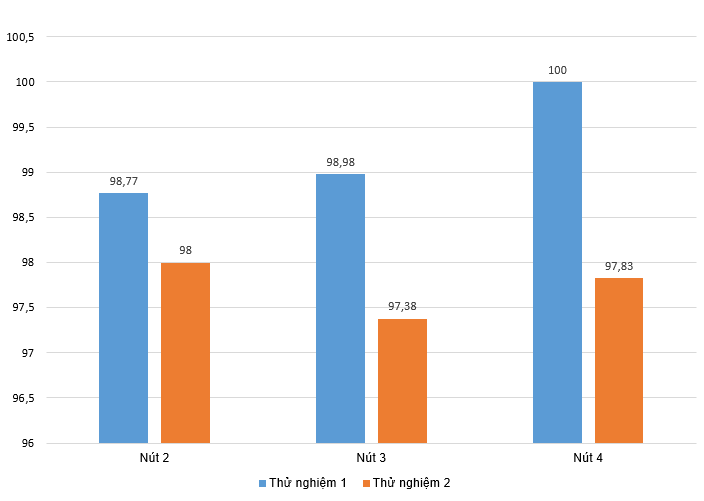
\includegraphics[scale=0.5]{image/sendrate}
\caption{Kết quả thí nghiệm đánh giá độ mất gói}
\label{sendrate}
\end{figure}
\subsubsection{Thử nghiệm 2: Đánh giá độ mất gói trong điều kiện thách thức}
Thử nghiệm 2 được thực hiện tại khuôn viên Đại học Bách Khoa Hà Nội, các thông số kỹ thuật của thử nghiệm 2 được thiết lập giống với thử nghiệm 1. Trong thử nghiệm này, Gateway được đặt tại tầng 6 thư viện Tạ Quang Bửu, nút đặt rải rác trong khuôn viên trường với môi trường có vật cản. Kết quả thử nghiệm 2 được ghi lại trong Bảng \ref{TN2} và được biểu diễn trên Hình \ref{sendrate}{}.\\
\begin{table}[h]
\centering
\caption{Bảng quả độ mất gói trong điều kiện thách thức}
\label{TN2}
\begin{tabular}{|c|c|c|c|}
\hline
 & Nút 2 & Nút 3 & Nút 4 \\
 \hline
 Gửi bản tin thành công & 98,0 \% & 97,38 \% & 97,83 \% \\
 \hline
 Hủy bản tin & 2,0 \% & 2,62 \% & 2,17 \% \\
 \hline
\end{tabular}
\end{table}
\subsubsection{Đánh giá kết quả thử nghiệm}
Trong cả 2 thử nghiệm, độ mất gói là rất nhỏ (nhỏ hơn 3\%) chứng tỏ thuật toán đa truy nhập hoạt động tốt với số lượng nút nhỏ (3 nút). Bên cạnh đó, tỷ lệ mất gói của thử nghiệm 2 cao hơn thử nghiệm 1, cho thấy được khoảng cách và vật cản có ảnh hưởng đến độ mất gói trong quá trình truyền dữ liệu.
\subsection{Hệ thống BKRES-LoRa}
Công nghệ LoRa đã được phòng nghiên cứu Sanslab áp dụng vào hệ thống BKRES thành công. Module truyền thông được tích hợp vào kit điều khiển (hình \ref{KitBKRES_LoRa}{}) với kích thước gọn nhẹ, tiêu tốn ít năng lượng (module sử dụng Pin để cung cấp năng lượng).
\par 
Những bản tin Gateway nhận được sẽ được gửi đến server và những dữ liệu đó được hiển thị các ứng dụng (hình \ref{Webapp}{}).\\
\begin{figure}[h]
\centering
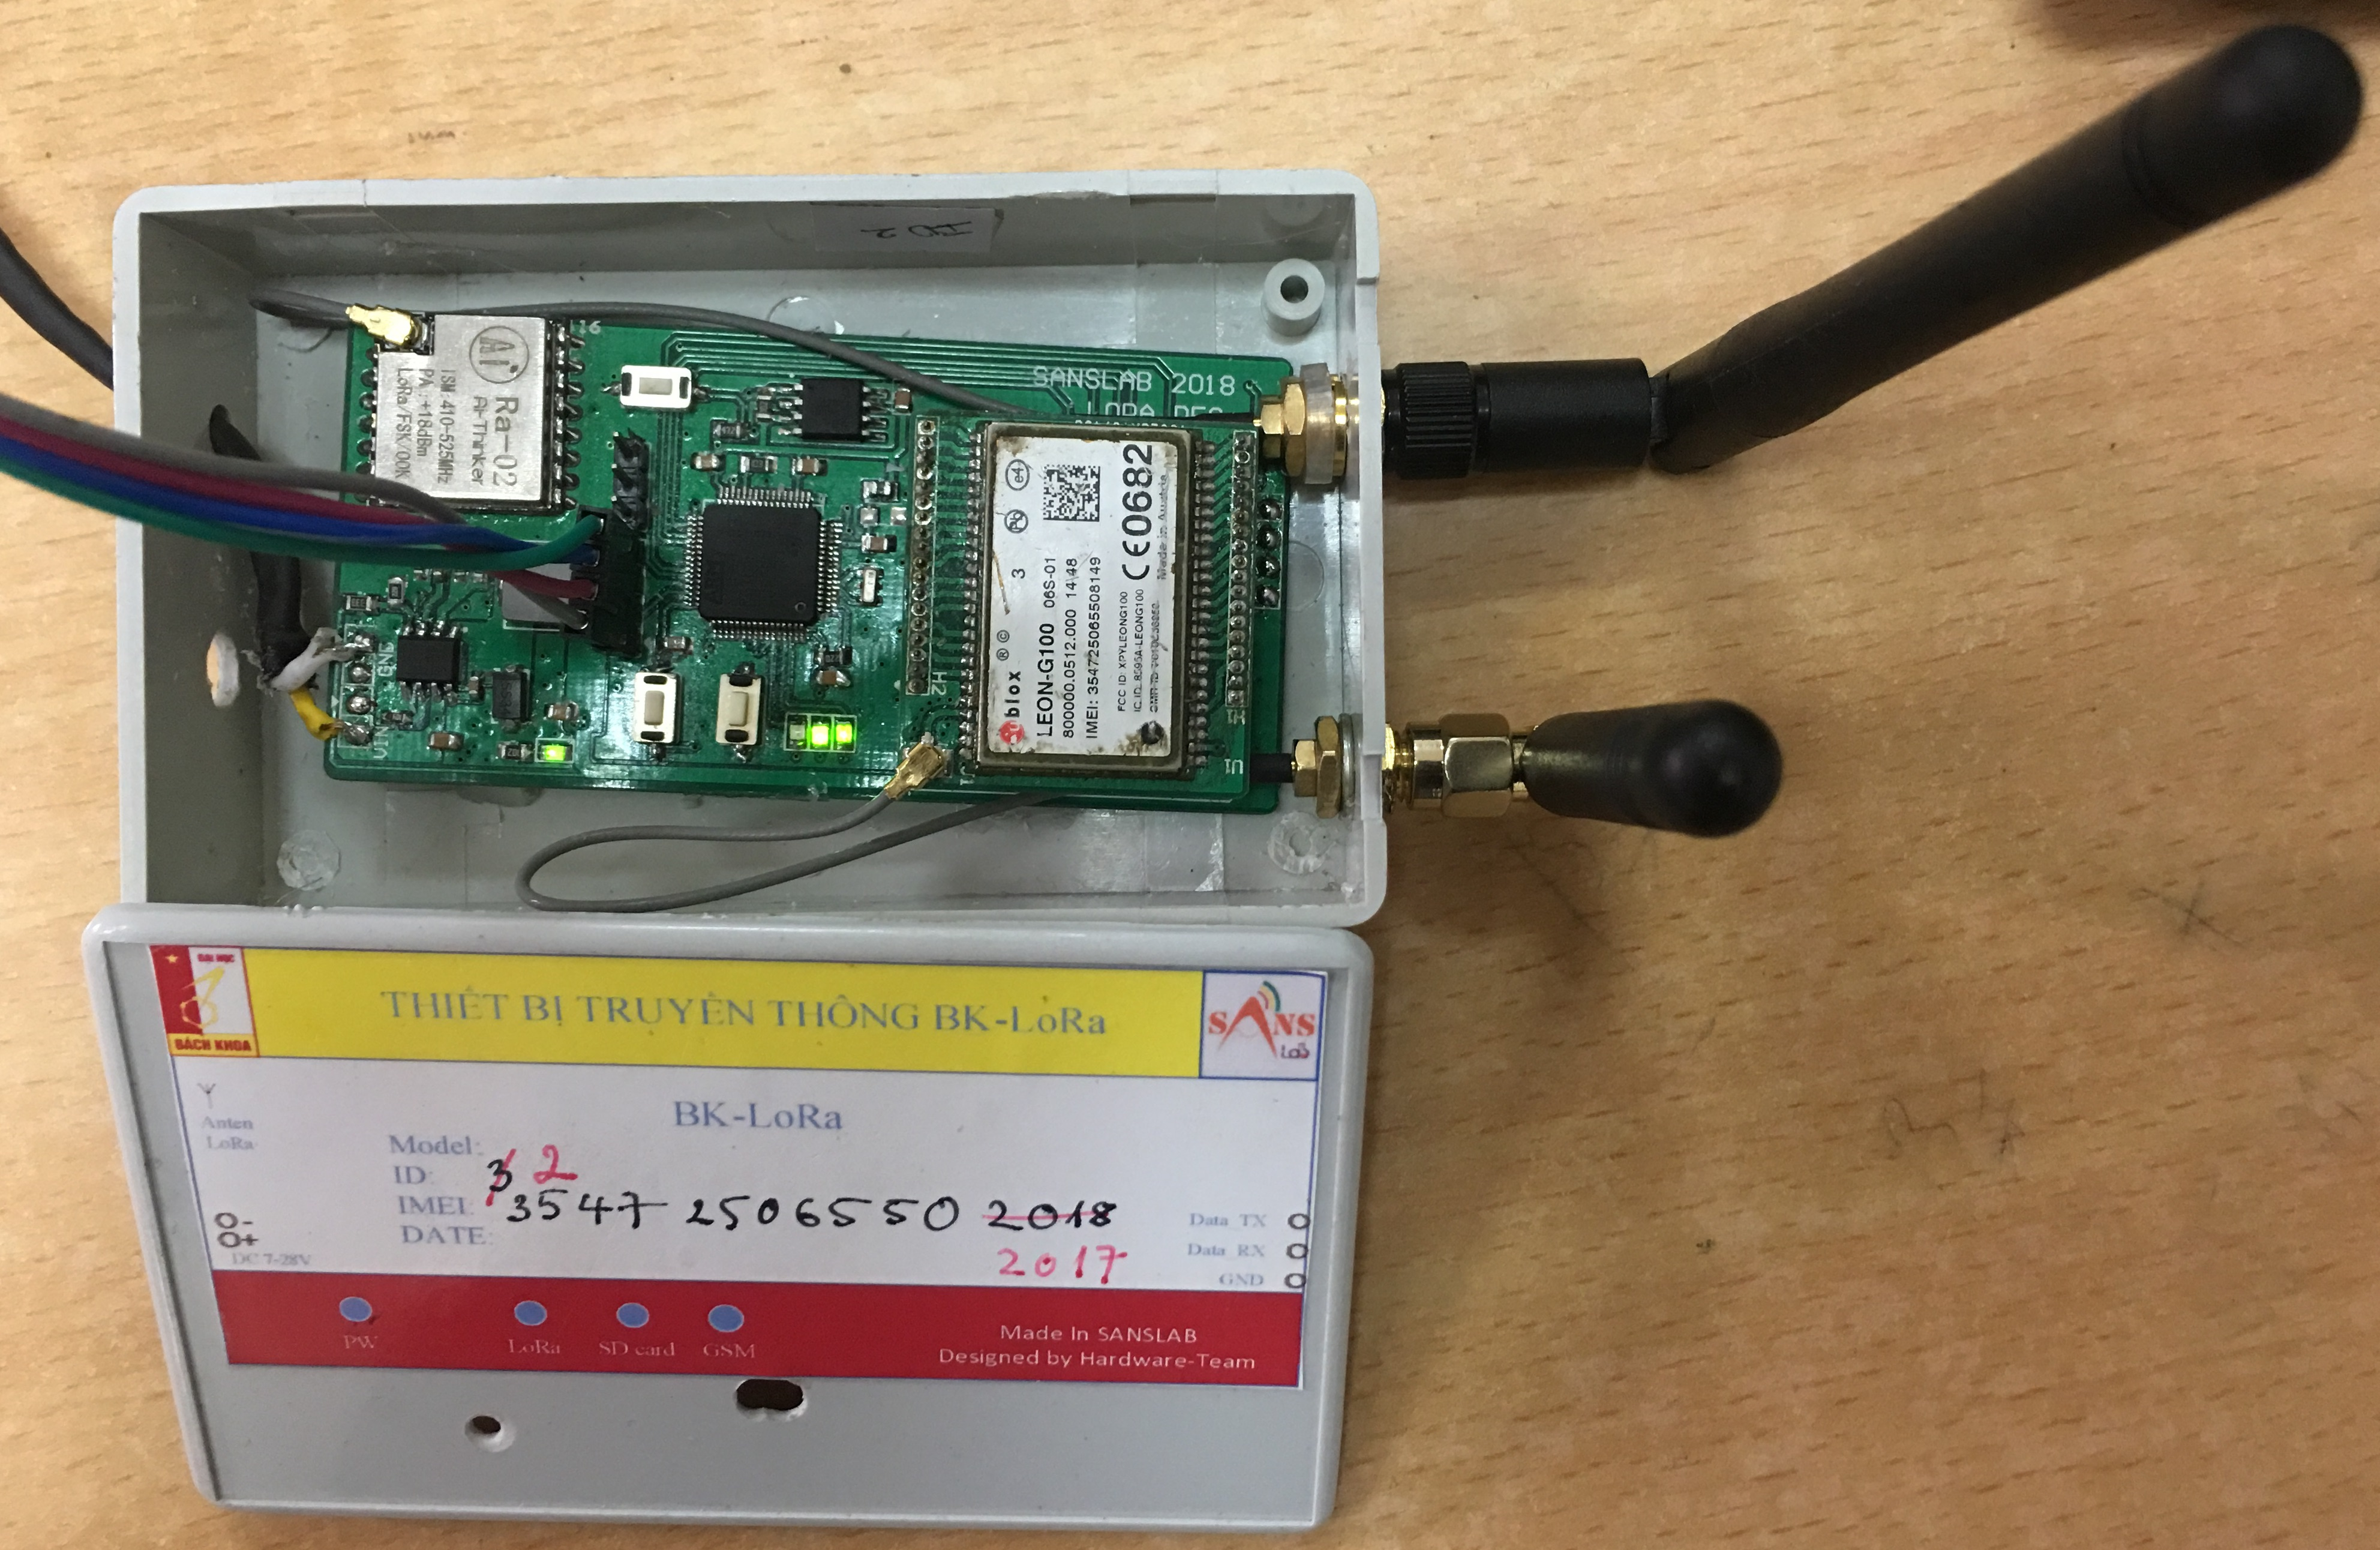
\includegraphics[scale=0.08]{image/KitBKRES_LoRa}
\caption{Kit điều khiển BKRES-LoRa}
\label{KitBKRES_LoRa}
\end{figure}\\
\begin{figure}[h]
\centering
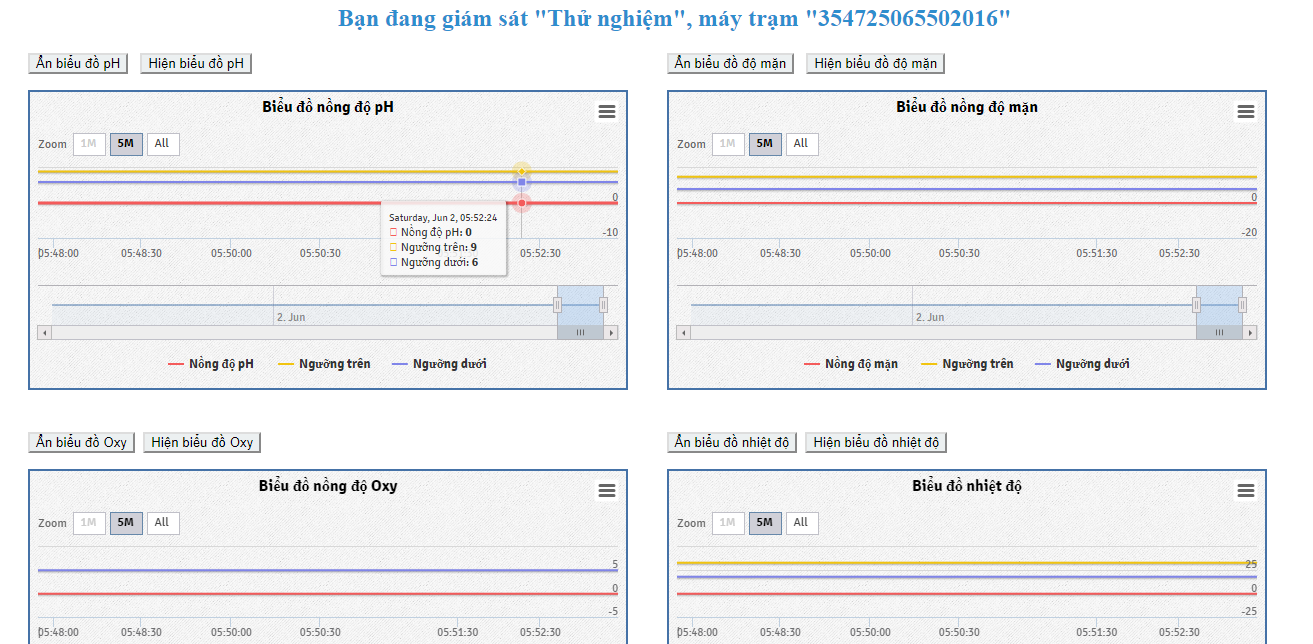
\includegraphics[scale=0.3]{image/application}
\caption{Hiển thị dữ liệu trên ứng dụng web}
\label{Webapp}
\end{figure}
\section{Đánh giá thuật toán và định hướng phát triển}
Thuật toán đa truy nhập có những ưu điểm và nhược điểm sau:
\begin{itemize}
\item Ưu điểm:
	\begin{itemize}
	\item	Thuật toán hoạt động tốt,
	\item	Hiệu năng truyền gói thành công cao hơn nhiều so với các giao thức truy nhập ngẫu nhiên khác,
	\item	Các thiết bị sử dụng thuật toán hoạt động ổn định, tiêu thụ ít năng lượng (so với sử dụng module sim).
	\end{itemize}
\item Nhược điểm:
	\begin{itemize}
	\item 	Chưa xác định được độ ảnh hưởng của số lượng thiết bị đến thuật toán,
	\item	Chưa xác định được các thời gian tiêu tốn để thực hiện các quá trình (tham gia mạng, gửi dữ liệu) để điều chỉnh trễ hợp lý,
	\item	Quá trình yêu cầu tham gia mạng phức tạp, ảnh hưởng đến quá trình gửi tin của nút khác,
	\item	Năng lượng tiêu thụ của Gateway lớn (vì Gateway không có khoảng thời gian để nghỉ),
	\item 	Hầu như chưa có sự quản lý của Gateway đối với các nút trong mạng.
	\end{itemize}
\end{itemize}
\par 
Thuật toán cần được phát triển hơn nữa để có thể tăng hiệu năng, độ ổn định của những thiết bị trong mạng và áp dụng cho mạng có số lượng nút lớn. Ngoài ra để tăng khoảng cách truyền, cần phát triển giao thức áp dụng cho mô hình mạng đa chặng để giảm số lượng Gateway trong mạng.
\section{Kết luận}
Qua kết quả của những thử nghiệm đã được tiến hành, chứng tỏ thuật toán đa truy nhập hoạt động tốt với số lượng nút nhỏ (3 nút), do điều kiện về số lượng thiết bị giới hạn nên em chưa xác định được kết quả hoạt động của thuật toán đa truy nhập trong mạng có số lượng nút lớn hơn. Ngoài ra, thuật toán đa truy nhập đã được thích hợp vào hệ thống BKRES-LoRa thành công.

\thispagestyle{plain}
\chapter*{Kết luận}
\addcontentsline{toc}{chapter}{Kết luận}
Sản phẩm của đồ án \textbf{"Thiết kế, phát triển giao thức đa truy nhập LoRa, tích hợp vào mạng WSN giám sát môi trường"} đã được thử nghiệm và tích hợp vào hệ thống BKRES-LoRa. Hệ thống BKRES-LoRa chuẩn bị được thực nghiệm trong môi trường thực tế. Nhờ đó, thuật toán đa truy nhập có thể phát hiện  những hạn chế còn tồn tại và sẽ được sửa chữa, cải thiện thêm. Trong tương lai, em tin hệ thống BKRES-LoRa sẽ được cải tiến ngày một tốt hơn để ngoài phục vụ cho lĩnh vực nghiên cứu, nó có thể trở thành một sản phẩm thương mai. Từ đó, hỗ trợ con người trong việc giám sát các thông số môi trường nói chung, cũng như giúp người nông dân trong quá trình nuôi tôm nói riêng.
\par 
Trong quá trình nghiên cứu, xây dựng và thiết kế sản phẩm, em đã vấp phải nhiều khó khăn. Nhưng nhờ có sự hướng dẫn tận tình của TS. Trần Quang Vinh cũng như sự giúp đỡ của các thành viên trong phòng nghiên cứu Sanslab đã giúp em hoàn thiện đồ án này. Qua đó, giúp em củng cố thêm những kiến thức về phần cứng, lập trình; những kỹ năng làm việc nhóm, tìm hiểu nghiên cứu những vấn đề mới; cũng như có được những kiến thức mới và trải nghiệm thực tế.
\thispagestyle{plain}
\addcontentsline{toc}{chapter}{Tài liệu tham khảo}
\begin{thebibliography}{20}
\bibitem{1}
https://www.i-scoop.eu/internet-of-things-guide/iot-network-lora-lorawan/ truy nhập cuối cùng ngày 12/03/2018.
\bibitem{2}
O. Khutsoane, B. Isong và A., “IoT Devieces and Appications based on LoRa/LoRaWAN”, Industrial Electronics Society, IECON 2017 – 43rd Annual Conference of the IEEE, Beijing, China, 29 Oct.-1 Nov. 2017.
\bibitem{3}
Guillaume Ferré, "Collision and Packet Loss Analysis in a LoRaWAN Network", 25th European Signal Processing Conference (EUSIPCO), 2017.
\bibitem{4}
Alexandru Lavric, Valentin Popa, “Internet of Things and LoRaTM Low-Power Wide-Area Networks: A Survey”, Signal, Cricuits and Systems (ISSCS), 2017 International Symposium on, Iasi, Romania, 13–14 July, 2017.
\bibitem{5}
U. Noreen, A. Bounceur và L. Clavier, "A Study of LoRa Low Power and Wide Area Network Technology", 3${rd}$ International Conference on Advanced Technologies for Signal and Image Processing - ATSIP, Fez, Morroco, May 22-24, 2017.
\bibitem{6}
Andrew S. Tanenbaum, David J. Wetherall, \textit{"Computer Network"}, Prentice Hall, 2010.
\bibitem{7}
Module LoRa Ra-02 SX1278 datasheet (https://www.en.ai-thinker.com).
\bibitem{8}
SX1276/77/78 datasheet (https://www.semtech.com).
\bibitem{9}
STM32F1xC, STM32F1xD, STM32F1xE datasheet (https://www.st.com).
\bibitem{10}
STM32Cube initialization code generator.
\end{thebibliography}
\thispagestyle{plain}
\chapter*{Phụ lục}
\addcontentsline{toc}{chapter}{Phụ Lục}
\changefontsizes{11pt}
%\begin{mybox}
\begin{center}
\changefontsizes{13pt}{\textbf{Hàm main của Gateway}}
\end{center}
\begin{lstlisting}
int main(void)
{
  /* Reset of all peripherals, Initializes the Flash interface and the Systick. */
  HAL_Init();
  /* Configure the system clock */
  SystemClock_Config();
  /* Initialize all configured peripherals */
  MX_GPIO_Init();
  MX_DMA_Init();
  MX_SPI3_Init();
  MX_USART1_UART_Init();
  /* USER CODE BEGIN 2 */
  SX1278_Config();
  /* USER CODE END 2 */
  while (1)
  {
	uint8_t e = receivePacketTimeoutACK (&hspi3, 10000);
	if (!e){
		UART_print ("\nReceive msg");
		char msg[40] = {0};
		for (uint8_t i = 0; i < packet_received.length; i++){
			msg[i] = (char)packet_received.data[i];
		}
		int ID = packet_received.src;
		if (msg[1] == 'D'){
			char title[100];
			sprintf(title, "\nReceive Data form node %d: ", ID);
			UART_print(title);
			UART_print(msg);
		}
		else checkNode(ID, msg);	
	}
	else UART_print ("\nDon't have msg");
  }
}
\end{lstlisting}
\newpage
\begin{center}
\changefontsizes{13pt}{\textbf{Hàm kiểm tra bản tin xác thực của Gateway}}
\end{center}
\begin{lstlisting}
void checkNode (int nodeAddr, char msg[]){
		char title[100];
		sprintf(title, "\nSend accepted Msg to Node %d", nodeAddr);
		char *response;
		uint8_t e;
		UART_print(title);
		if (msg[2] == 's' && msg[3] == 'a' && msg[4] == 'n' && msg[5] == 's' && msg[6] == 'l' && msg[7] == 'a' && msg[8] == 'b'){
			response = "1";
			UART_print ("\nGateway: 1");
			arrNodeAddr[numberofNode++] = nodeAddr;
		}
		else{
			response = "0";
			UART_print ("\nGateway: 0");
		}
		uint8_t cnt;
		do{ 
			e = sendPacketTimeoutACKRetries(&hspi3, nodeAddr, response);
			cnt++;
			HAL_Delay (5);
		}
		while (e > 0 && cnt < 3);
}
\end{lstlisting}
\newpage
\begin{center}
\changefontsizes{13pt}{\textbf{Hàm main của nút}}
\end{center}
\begin{lstlisting}
int main(void)
{
  /* MCU Configuration----------------------------------------------------------*/
  /* Reset of all peripherals, Initializes the Flash interface and the Systick. */
  HAL_Init();
  /* Configure the system clock */
  SystemClock_Config();
  /* Initialize all configured peripherals */
  MX_GPIO_Init();
  MX_DMA_Init();
  MX_SPI3_Init();
  MX_USART1_UART_Init();
  /* USER CODE BEGIN 2 */
  SX1278_Config();
  /* USER CODE END 2 */
	delay = NODE_ADDRESS * 10;
	requestJoinNetwork(GWAY_ADDRESS);
  while (1)
  {
  /* USER CODE END WHILE */
		if (joinedNetwork == 1)
				sendData(GWAY_ADDRESS);
		HAL_Delay(15000);
  /* USER CODE BEGIN 3 */
  }
}
\end{lstlisting}
\newpage
\begin{center}
\changefontsizes{13pt}{\textbf{Hàm yêu cầu tham gia mạng của nút}}
\end{center}
\begin{lstlisting}
void requestJoinNetwork (uint8_t GWaddr)
{
		char msgRQ[20] = "@Rsanslab";
		uint8_t e;
		do{
				e	= sendPacketTimeoutACK (&hspi3, GWaddr , msgRQ);
				if (e == 0){
						UART_print ("\nSend msg_request successful, waiting msg_acception");
						uint8_t state = receivePacketTimeoutACK (&hspi3, 10000);
						char msgAccept[10] = {0};
						if (state == 0 && packet_received.src == GWAY_ADDRESS){
							for (uint8_t i = 0; i < packet_received.length; i++){
									msgAccept[i] = (char) packet_received.data[i];
							}
							if (msgAccept[0] == '1'){
									UART_print ("\nGateway accepted");
									joinedNetwork = 1;
							}
							else{
									UART_print ("\nGateway didn't accept");
									joinedNetwork = 2;
							}
							//delay = NODE_ADDRESS * 10;
						}
				}
				else{
					UART_print("\nSend msg_request nonsuccessful");
					//int x = rand() % 10;
					HAL_Delay (1000);
					//delay *= 2;
				}
		}
		while (e);
}
\end{lstlisting}
\newpage
\begin{center}
\changefontsizes{13pt}{\textbf{Hàm gửi dữ liệu của nút}}
\end{center}
\begin{lstlisting}
void sendData (uint8_t GWAddr){
		char msgData[100] = "@DN045<~1Gq!J1,UaD2)R'I0f(O='UY5E$cWE>!!!!d!!!!g!!!!f!!!!c!!!!b!!!!~>";
		//sprintf(msgData, "", counter);
		delay = 10 * NODE_ADDRESS;
		uint8_t e;
		uint8_t cnt = 0;
		do{
				e = sendPacketTimeoutACK(&hspi3, GWAddr, msgData);
				cnt_sent++;
				cnt++;
				if (e > 0){
					//int x = rand() % 10;
					HAL_Delay (delay);
					if (delay *2 < 2000) delay *= 2;
				}
				else
					counter++;
		}
		while(e && cnt < 5);
		char tmp[100];
		if (e == 0){
			sprintf(tmp, "\nNode %d :received %d, retries %d, deleted %d, sent %d",NODE_ADDRESS, counter, cnt, cnt_huy_goi, cnt_sent);
			UART_print(tmp);
			}
		else 
			cnt_huy_goi++;
}
\end{lstlisting}
\printbibliography
\end{document}